
\documentclass[11pt,spanish,
		listoftables,listoffigures]
		{tfgplantilla}


\usepackage[utf8]{inputenc} 

\usepackage{lipsum}

\usepackage{wrapfig}

\usepackage{float}


\title{Desarrollo de un app para el \\
         tratamiento de las Enfermedades Cardiovasculares}
\author{Ricardo Cajigas Arenas \\ José Ángel Sánchez Martín}
\tutor{José Ignacio Hidalgo Pérez}
\curs{2016-2017}


\keywords{Enfermedades cardiovasculares, Aplicación móvil, Diabetes, Colesterol, Tabaquismo, Obesidad, Hipertensión Arterial, Riesgo Cardiovascular}              % Palabras clave
     	      {Cardiovascular Diseases, Mobile Application, Diabetes, Cholesterol, Smoking, Obesity, Arterial Hypertension, Cardiovascular Risk}        			  % Key words

\begin{document}

%%%%%%%%%%%%%%%%%%%%%%%%%%%%%%%%%%%%%%%%%%%%%%%%%%%%%%%%%%%%%%%%%%%%%%%%%%%%%%%%%%%%%%%%%%%%%%%%%%%%%%%%%%%%%%%%%%%%%%%%%
%																	     AUTORIZACIÓN DE DIFUSIÓN		                       															  %
%%%%%%%%%%%%%%%%%%%%%%%%%%%%%%%%%%%%%%%%%%%%%%%%%%%%%%%%%%%%%%%%%%%%%%%%%%%%%%%%%%%%%%%%%%%%%%%%%%%%%%%%%%%%%%%%%%%%%%%%%
%\chapter{Autorización de difusión}
%\cleardoublepage

%%%%%%%%%%%%%%%%%%%%%%%%%%%%%%%%%%%%%%%%%%%%%%%%%%%%%%%%%%%%%%%%%%%%%%%%%%%%%%%%%%%%%%%%%%%%%%%%%%%%%%%%%%%%%%%%%%%%%%%%%
%																		   AGRADECIMIENTOS				                     															  %
%%%%%%%%%%%%%%%%%%%%%%%%%%%%%%%%%%%%%%%%%%%%%%%%%%%%%%%%%%%%%%%%%%%%%%%%%%%%%%%%%%%%%%%%%%%%%%%%%%%%%%%%%%%%%%%%%%%%%%%%%
%\chapter{Agradecimientos}
%\cleardoublepage

%%%%%%%%%%%%%%%%%%%%%%%%%%%%%%%%%%%%%%%%%%%%%%%%%%%%%%%%%%%%%%%%%%%%%%%%%%%%%%%%%%%%%%%%%%%%%%%%%%%%%%%%%%%%%%%%%%%%%%%%%
%																			PROLOGO					                     															  %
%%%%%%%%%%%%%%%%%%%%%%%%%%%%%%%%%%%%%%%%%%%%%%%%%%%%%%%%%%%%%%%%%%%%%%%%%%%%%%%%%%%%%%%%%%%%%%%%%%%%%%%%%%%%%%%%%%%%%%%%%
%\chapter{Prólogo}
%\cleardoublepage

%%%%%%%%%%%%%%%%%%%%%%%%%%%%%%%%%%%%%%%%%%%%%%%%%%%%%%%%%%%%%%%%%%%%%%%%%%%%%%%%%%%%%%%%%%%%%%%%%%%%%%%%%%%%%%%%%%%%%%%%%
%																			RESUMEN					                     															  %
%%%%%%%%%%%%%%%%%%%%%%%%%%%%%%%%%%%%%%%%%%%%%%%%%%%%%%%%%%%%%%%%%%%%%%%%%%%%%%%%%%%%%%%%%%%%%%%%%%%%%%%%%%%%%%%%%%%%%%%%%
\begin{abstract}
\setcounter{page}{1}
\addcontentsline{toc}{chapter}{Resumen}
El uso de aplicaciones en dispositivos móviles ha ido creciendo con el paso de los años, siendo hoy en día una herramienta fundamental en un amplio ámbito, desde profesionales como son las comunicaciones, economía, comercio, salud hasta las destinadas al ocio, viajes, deportes...

Esta aplicación para Android está enfocada en el ámbito de la medicina, dando solución a uno de los problemas actuales que existe en el Hospital Virgen de la Salud de Toledo, a través de una interfaz intuitiva y simple, proporcionando agilidad al médico en el cálculo del riesgo cardiovascular y asistencia complementaria a los métodos convencionales.

Enfocada para ser gestionada por los médicos, permitiéndoles almacenar los datos actuales de un paciente como son hipertensión arterial, colesterol, diabetes, tabaquismo e índice de masa corporal. Para más tarde obtener el riesgo cardiovascular del mismo y facilitar un tratamiento inicial al médico.
\end{abstract}

\begin{abstract}[english]
\addcontentsline{toc}{chapter}{Abstract}
The use of applications in mobile devices has been growing over the years, and is nowadays a fundamental tool in a wide range, from professionals such as communications, economics, commerce, health or destined to the leisure, travel , sports...

This application for Android is focused on the field of medicine, giving the solution to one of the current problems that existed in the Hospital Virgen de la Salud of Toledo through, an intuitive and simple interface, providing agility to the doctor in calculating the cardiovascular risk, while being complemented by conventional methods.

Intended to be managed by doctors, allowing them to store a patient's current data such as high blood pressure, cholesterol, diabetes, smoking and body mass index. In order to later obtain the cardiovascular risk of the same and facilitate an initial treatment to the doctor.
\end{abstract}

\mainmatter

%%%%%%%%%%%%%%%%%%%%%%%%%%%%%%%%%%%%%%%%%%%%%%%%%%%%%%%%%%%%%%%%%%%%%%%%%%%%%%%%%%%%%%%%%%%%%%%%%%%%%%%%%%%%%%%%%%%%%%%%%
%																	INTRODUCCIÓN EN ESPAÑOL																				  %
%%%%%%%%%%%%%%%%%%%%%%%%%%%%%%%%%%%%%%%%%%%%%%%%%%%%%%%%%%%%%%%%%%%%%%%%%%%%%%%%%%%%%%%%%%%%%%%%%%%%%%%%%%%%%%%%%%%%%%%%%
\chapter{Introducci\'on}

La constante evolución hacia una sociedad más conectada para conseguir soluciones a problemas informatizando los procesos y métodos e ir acercándonos a los términos de IoT, SmartCities...

Con esta idea en mente y tras una reunión con el médico Rafael Rubio Díaz nos enfocamos en la diabetes como punto de partida. Tenían el propósito de conseguir mejorar el proceso de tratamiento de información en pacientes con diabetes para ir dejando atrás los métodos convencionales, escribir los informes médicos en el ordenador de su despacho, para llegar a tener un mecanismo que les permitiera no estar atados a su ordenador y se pudieran mover por el hospital consiguiendo el mismo fin. 

Finalmente se decidió expandir el proyecto a los factores de riesgo cardiovasculares para tener una aplicación más completa y robusta, y obtener un tratamiento con mayor precisión, a los médicos poseer mayor información del paciente.

Surge este proyecto como Trabajo Fin de Grado correspondiente al Grado en Ingeniería Informática, con la firme idea de desarrollar una aplicación móvil que fuera capaz de ayudar en el marco de la sanidad, dando rapidez en el cálculo del riesgo cardiovascular de los pacientes.

%MOTIVACION
\section{Motivaci\'on}

Queríamos llevar a cabo un proyecto que no se quedara solo con fines académicos, sino que además fuera de utilidad para un colectivo de la sociedad. 

Decidimos centrarnos en la rama de la sanidad por varios factores influyentes, al tratarse de un ámbito que nos parecía muy interesante y no estaba tan a la vanguardia como otras ramas y que no existían muchas aplicaciones en el mercado que cubrieran esta necesidad en específico. 
Esta aplicación permitiría al médico calcular el riesgo cardiovascular y almacenar los datos médicos actuales del paciente, pero dotándole de mayor libertad y prontitud al mismo tiempo que ir acercándoles a las nuevas tecnologías.
\vfill

%OBJETIVOS
\section{Objetivos}

El objetivo general del proyecto es desarrollar una herramienta, una aplicación móvil, que facilite el trabajo del personal sanitario en el cálculo del riesgo cardiovascular, almacenamiento de datos del paciente y posterior tratamiento.

El presente Trabajo Fin de Grado tiene los siguientes objetivos:
\begin{itemize}
	\item Realizar un estudio de los factores de riesgo cardiovascular, para clasificarlos y obtener los que sean más relevantes para el posterior cálculo del riesgo cardiovascular.
	\item Diseñar y elaborar una aplicación móvil que sea práctica para el usuario, atractiva visualmente e intuitiva.
	\item Obtener a partir de todos los datos introducidos de un paciente, el índice de riesgo cardiovascular y un tratamiento inicial.
\end{itemize}

%ESTADO DEL ARTE
\section{Estado del arte}

Con el fin de determinar el grado de impacto que pueda tener este proyecto, hemos realizado una investigación de posibles aplicaciones con objetivos o rasgos similares. Nuestro estudio ha revelado la existencia de varias aplicaciones con rasgos similares, o metas semejantes a las planeadas por nuestra aplicación. Citamos a continuación varios de los potenciales competidores:

\noindent
\textbf {Appteca }

\includegraphics[height=0.7cm]{hipertension_icon.jpg}

\includegraphics[height=0.7cm]{riesgo-cardiovascular_icon.jpg}  

\noindent
Es un  proyecto llevado a cabo por Sociedad Española de Cardiología y la Sociedad Española de Medicina, en las que incluyen varias aplicaciones relacionadas con el riesgo cardiovascular; Riesgo cardiovascular e Hipertensión arterial.

\noindent
\textbf {PSCV}

\includegraphics[height=0.7cm]{PSCV_icon.jpg}

\noindent
Permite calcular una aproximación del riesgo cardiovascular con los fines y tratamientos asociados a cada nivel de riesgo. Ofrece información sobre el diagnóstico, manejo y seguimiento en la diabetes tipo 2, hipertensión arterial, infarto agudo al miocardio...

\noindent
\textbf {ASCVD Risk Estimator}
\ 
\includegraphics[height=0.7cm]{ASCVD_icon.jpg}

\noindent
Proporciona acceso rápido a recomendaciones específicas para los riesgos estimados por el calculador a la vez que vez que referencia información relacionado con terapia, monitorización y estilo de vida que puede interesar a pacientes y médicos.

\bigskip

En definitiva, hay varias aplicaciones con una meta temática afín. No obstante, nuestra aplicación presenta funcionalidades únicas no cubiertas por las mencionadas anteriormente que le proporciona un carácter innovador. 

\vfill
%ESTRUCTURA DE LA MEMORIA
\section{Estructura de la mem\'oria}

La memoria está organizada en cinco capítulos siendo el primero de estos la presente introducción.

En el capítulo 2 se hace una explicación detallada de las funcionalidades de la aplicación móvil. Incluyendo los respectivos diagramas de actividades y ventana correspondiente de cada uno de ellos.

El capítulo 3 presenta los módulos que conforman el sistema.

El capítulo 4 se detalla la estructura de la base de datos empleada.

El capítulo 5 presenta las tecnologías empleadas acompañadas de una breve descripción y características.

En el capítulo 6 se presentan las principales conclusiones de este trabajo. En un último lugar se listan las mejoras que se podrían realizar con el fin de incrementar sus funcionalidades y acrecentar su competitividad en el mercado.


%%%%%%%%%%%%%%%%%%%%%%%%%%%%%%%%%%%%%%%%%%%%%%%%%%%%%%%%%%%%%%%%%%%%%%%%%%%%%%%%%%%%%%%%%%%%%%%%%%%%%%%%%%%%%%%%%%%%%%%%%
%																	INTRODUCCIÓN EN INGLÉS																				  %
%%%%%%%%%%%%%%%%%%%%%%%%%%%%%%%%%%%%%%%%%%%%%%%%%%%%%%%%%%%%%%%%%%%%%%%%%%%%%%%%%%%%%%%%%%%%%%%%%%%%%%%%%%%%%%%%%%%%%%%%%
%Solucionar
\addtocounter{chapter}{-1}
\selectlanguage{english}
\chapter{Introduction}
\phantomsection

The constant evolution towards a more connected society to get solutions to problems by computerizing the processes and methods and getting closer to the terms of IoT, SmartCities ...

With this idea in mind and after a meeting with the doctor Rafael Rubio Diaz we focus on diabetes as a starting point. They were intended to improve the process of information processing in patients with diabetes to go beyond conventional methods, write medical reports on the computer in their office, to have a mechanism that would allow them not to be tied to their computer and could move around the hospital getting the same end.

Finally, it was decided to expand the project to cardiovascular risk factors to have a more complete and robust application, and to obtain a treatment with more precision, to the doctors to possess more information of the patient.

This project emerges as a Degree Final Work corresponding to the Degree in Computer Engineering, with the firm idea of developing a mobile application that would be able to help within the healthcare framework, giving rapid calculation in the cardiovascular risk of patients.

%MOTIVATION
\section{Motivation}

We wanted to carry out a project that was not only for academic purposes, but was also of no use to a group of society.

We decided to focus on the health sector by several influential factors, as it was a field that we found very interesting and was not as cutting edge as other branches and that there were many applications in the market that covered this specific need.
This application would allow the physician to calculate the cardiovascular risk and store the patient's current medical data, but giving him greater freedom and promptness at the same time as approaching the new technologies.

\vfill
%OBJECTIVES
\section{Objectives}

The overall objective of the project is to develop a tool, a mobile application, that facilitates the work of health personnel in the calculation of cardiovascular risk, storage of patient data and subsequent treatment.

The present Work End of Degree has the following objectives:
\begin{itemize}
	\item Carry out a study of cardiovascular risk factors, to classify them and obtain those that are most relevant for the subsequent calculation of cardiovascular risk.
	\item Design and build a mobile application that is user-friendly, visually appealing and intuitive.
	\item Obtain from all the entered data of a patient, the cardiovascular risk index and an initial treatment.
\end{itemize}

%STATE OF THE ART
\section{State of the art}

In order to determine the degree of impact that this project may have, we have carried out an investigation of possible applications with similar objectives or traits. Our study has revealed the existence of several applications with similar traits, or goals similar to those planned by our application. We cite below several of the potential competitors:

\noindent
\textbf {Appteca }

\includegraphics[height=0.7cm]{hipertension_icon.jpg}

\includegraphics[height=0.7cm]{riesgo-cardiovascular_icon.jpg}  

\noindent
It is a project carried out by the Spanish Society of Cardiology and the Spanish Society of Medicine, which include several applications related to cardiovascular risk; Cardiovascular risk and Hypertension.

\noindent
\textbf {PSCV}

\includegraphics[height=0.7cm]{PSCV_icon.jpg}

\noindent
It allows to calculate an approximation of the cardiovascular risk with the purposes and treatments associated to each level of risk. It offers information on the diagnosis, management and follow-up in type 2 diabetes, hypertension, myocardial infarction ...

\noindent
\textbf {ASCVD Risk Estimator}

\includegraphics[height=0.7cm]{ASCVD_icon.jpg}

\noindent
It provides quick access to specific recommendations for the calculator's estimated risks, while referring to information related to therapy, monitoring and lifestyle that may be of interest to patients and physicians.

\bigskip

In short, there are several applications with a related thematic goal. However, our application presents unique functionalities not covered by the aforementioned that provides an innovative character. 

\vfill
%MEMORY STRUCTURE
\section{Memory structure}

The memory is organized in five chapters and the first of these is the present introduction.

Chapter 2 provides a detailed explanation of the features of the mobile application. Including the respective activity diagrams of each of them.

Chapter 3 presents the modules that make up the system.

Chapter 4 details the structure of the database used.

Chapter 5 presents the technologies used, accompanied by a brief description and characteristics.

In chapter 6 the main conclusions of this work are presented. Finally, we list the improvements that could be made in order to increase its functionality and increase its competitiveness in the market.

%%%%%%%%%%%%%%%%%%%%%%%%%%%%%%%%%%%%%%%%%%%%%%%%%%%%%%%%%%%%%%%%%%%%%%%%%%%%%%%%%%%%%%%%%%%%%%%%%%%%%%%%%%%%%%%%%%%%%%%%%
%																	ESPECIFICACIÓN DE LA APLICACION																			  %
%%%%%%%%%%%%%%%%%%%%%%%%%%%%%%%%%%%%%%%%%%%%%%%%%%%%%%%%%%%%%%%%%%%%%%%%%%%%%%%%%%%%%%%%%%%%%%%%%%%%%%%%%%%%%%%%%%%%%%%%%
\selectlanguage{spanish}
\chapter{Especificación de la aplicaci\'on}

En esta sección vamos a introducir las funciones desempeñadas por nuestra aplicación. Los cometidos primordiales de la misma son dar de alta a los pacientes, deducir su índice de riesgo cardiovascular y ofrecer una base para establecer el tratamiento.

Asimismo, la aplicación presenta un amplio rango de funcionalidades que describiremos en detalle en los puntos posteriores.

%%%%%%%%%%%MEDICO
\section {Compentencias disponibles para el médico}
Una responsabilidad característica del profesional sanitario es la aportación datos para el alta del paciente. Este rol requiere de un método (Mi perfil) que le conceda la capacidad de manipular sus datos personales.
Con el fin de asistir al médico en el diagnostico del tratamiento se facilita el acceso a una BD de fármacos. Si desea constatar que los resultados obtenidos reponden a una imagen verídica, o simplemente analizar la exactitud de las fórmulas empleadas, se introduce la pestaña de algorítmos.

Las interacciones que puede llevar a cabo exclusivamente el personal médico se ilustra en el siguiente diagrama.

\begin{figure}[H]
\centering
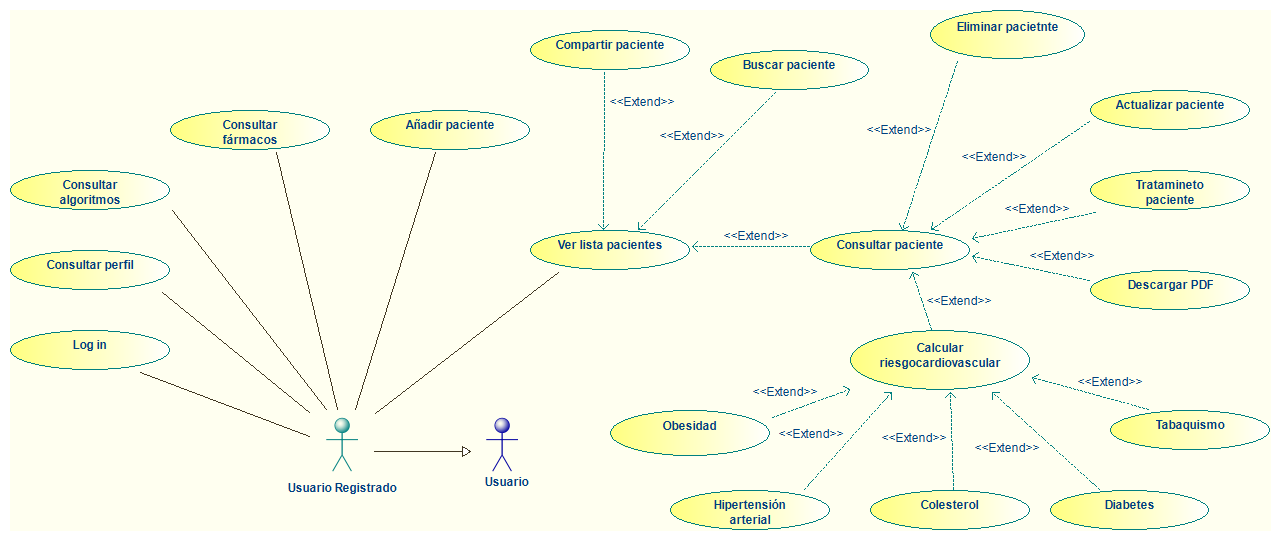
\includegraphics[height= 6cm]{diagramas/UsuarioRegistradoUseCasediagram.png}
\caption{Diagrama de caso de uso - Usuario Registrado}
\end{figure}

%NUEVO PACIENTE
\subsection {Nuevo paciente}

Inscribe los datos de un nuevo paciente bajo el médico logueado. Para ello se le identificará mediante un ID que responderá a la siguiente formula; las iniciales del nombre y apellidos seguido de su fecha de nacimiento en formato ddmmyy. También se facilitará la información relativa al sexo.

*En aquellos casos en los que el paciente no disponga de dos apellidos, se repetirá la inicial del primer apellido dos veces. Es importante mencionar que este sistema no trata aquellos individuos que excedan los dos dígitos de edad.

\begin{figure}[H]
\centering
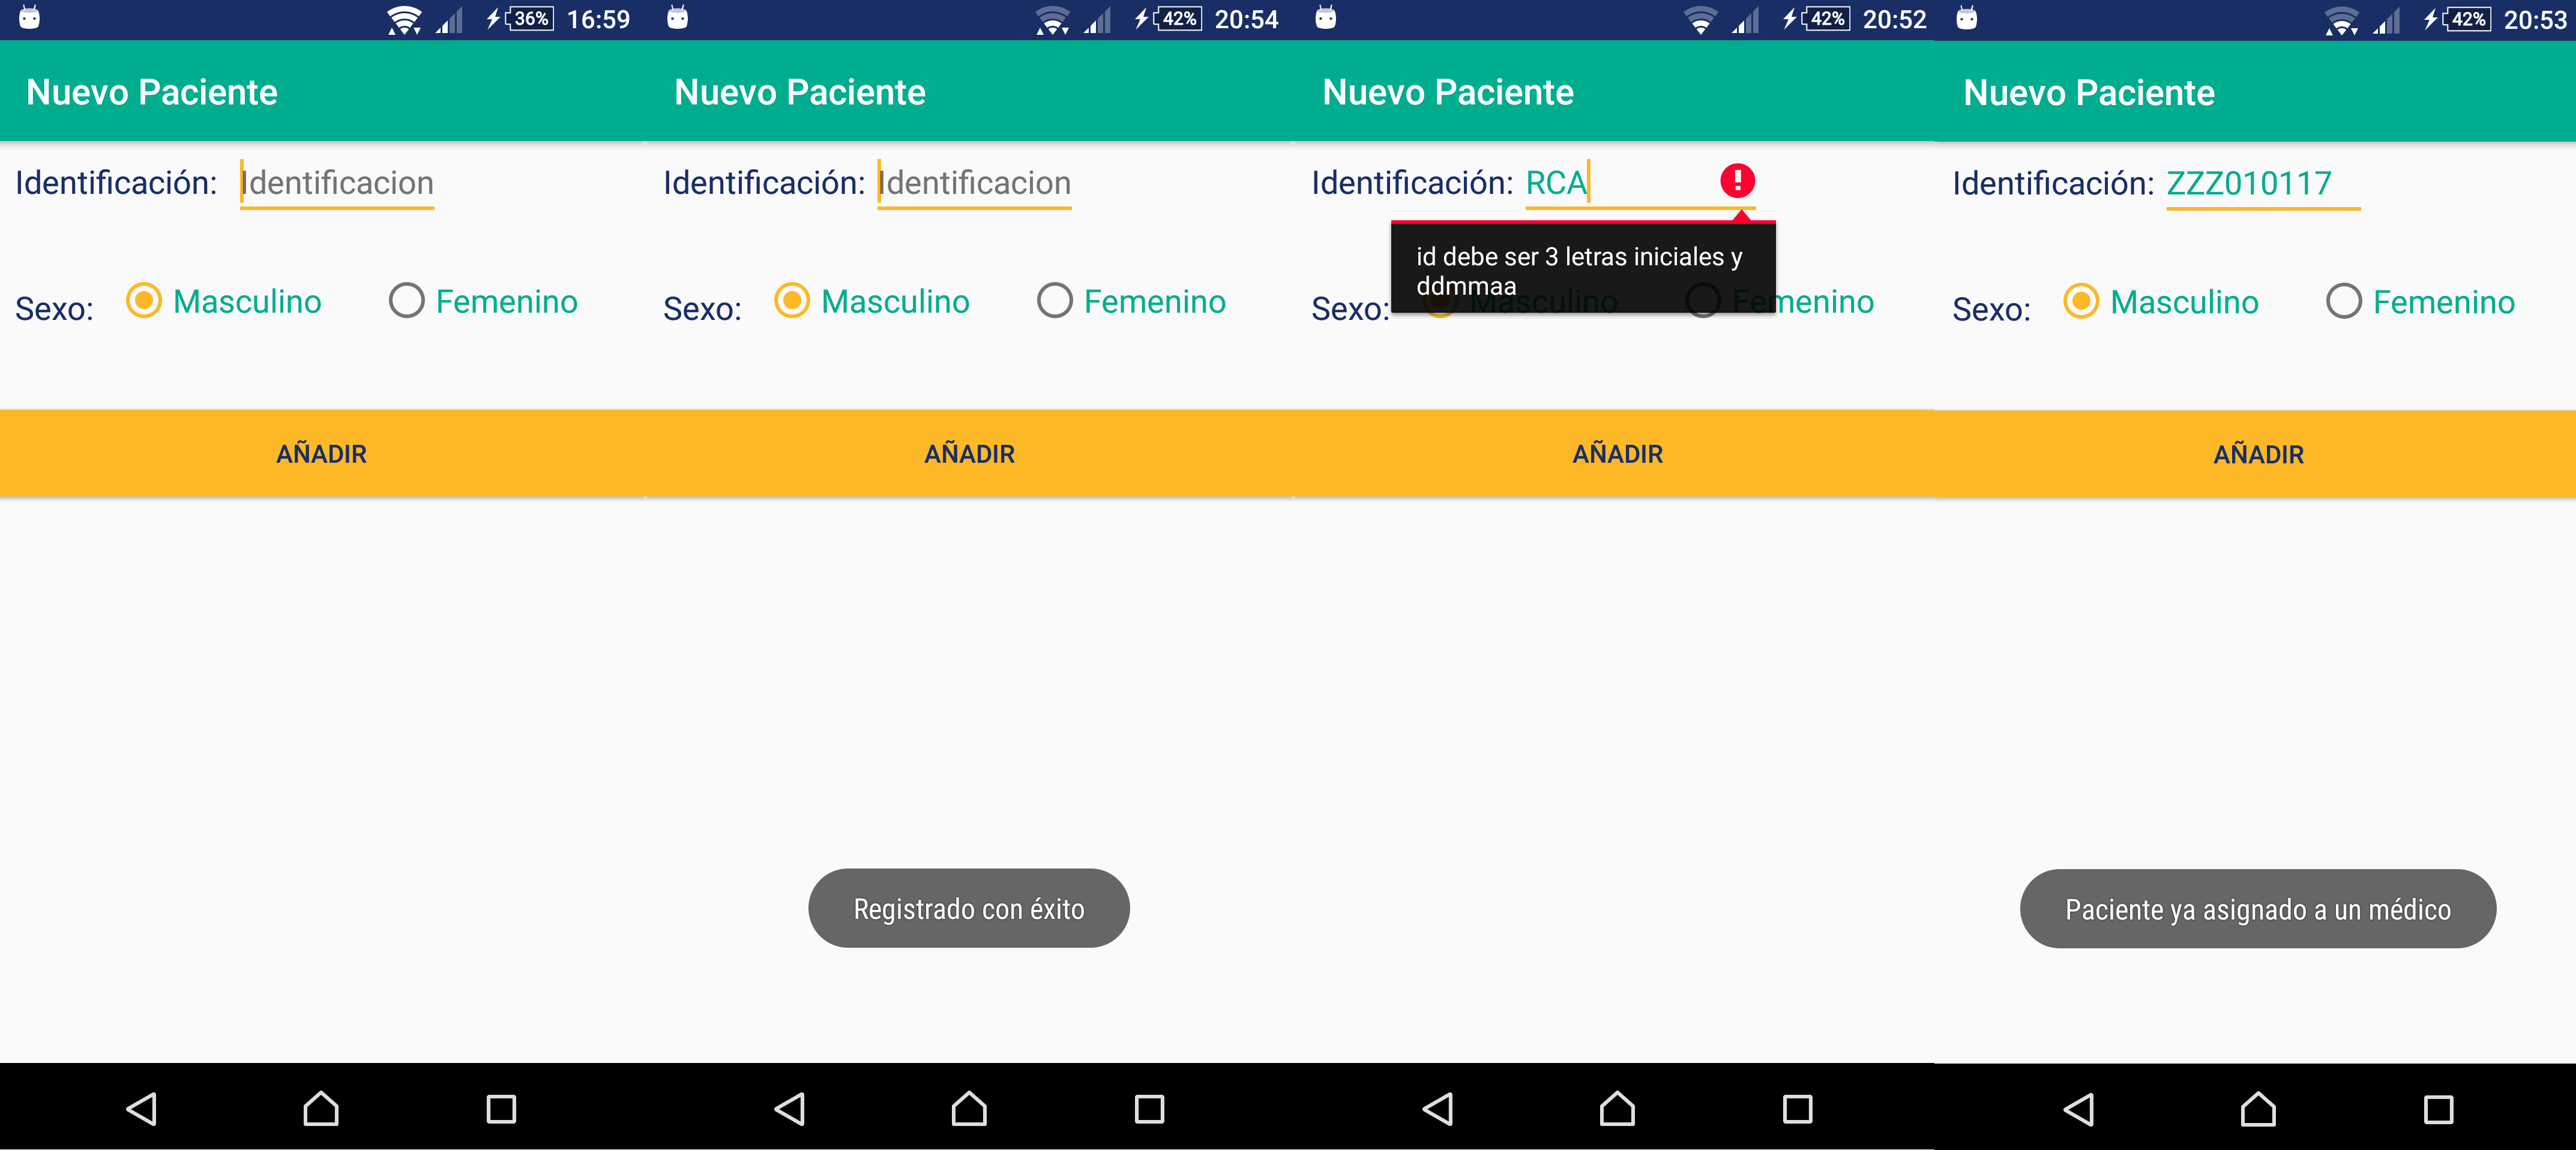
\includegraphics[height= 6.7cm]{capturas/nuevoPacienteFull.png}
\caption{Ventana - Nuevo Paciente}
\end{figure}

\begin{figure}[H]
\centering
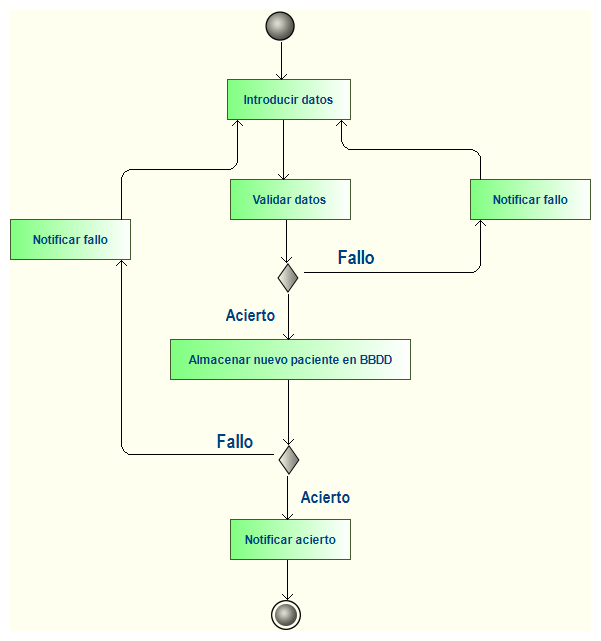
\includegraphics[height= 11cm]{diagramas/AnadirpacienteActivitydiagram.png}
\caption{Diagrama de actividad - Nuevo Paciente}
\end{figure}

%CONSULTAR ALGORITMOS
\subsection {Consultar algorítmos}

Permite asesorarse sobre nuestras formulas automatizadas de las que hacemos uso para calcular los resultados de los factores de influencia en el cálculo del riesgo cardiovascular: diabetes, colesterol, hipertensión arterial, índice de masa corporal, tabaquismo.
Los algoritmos se presentan gráficamente en diagramas de flujo.

\begin{figure}[H]
\centering
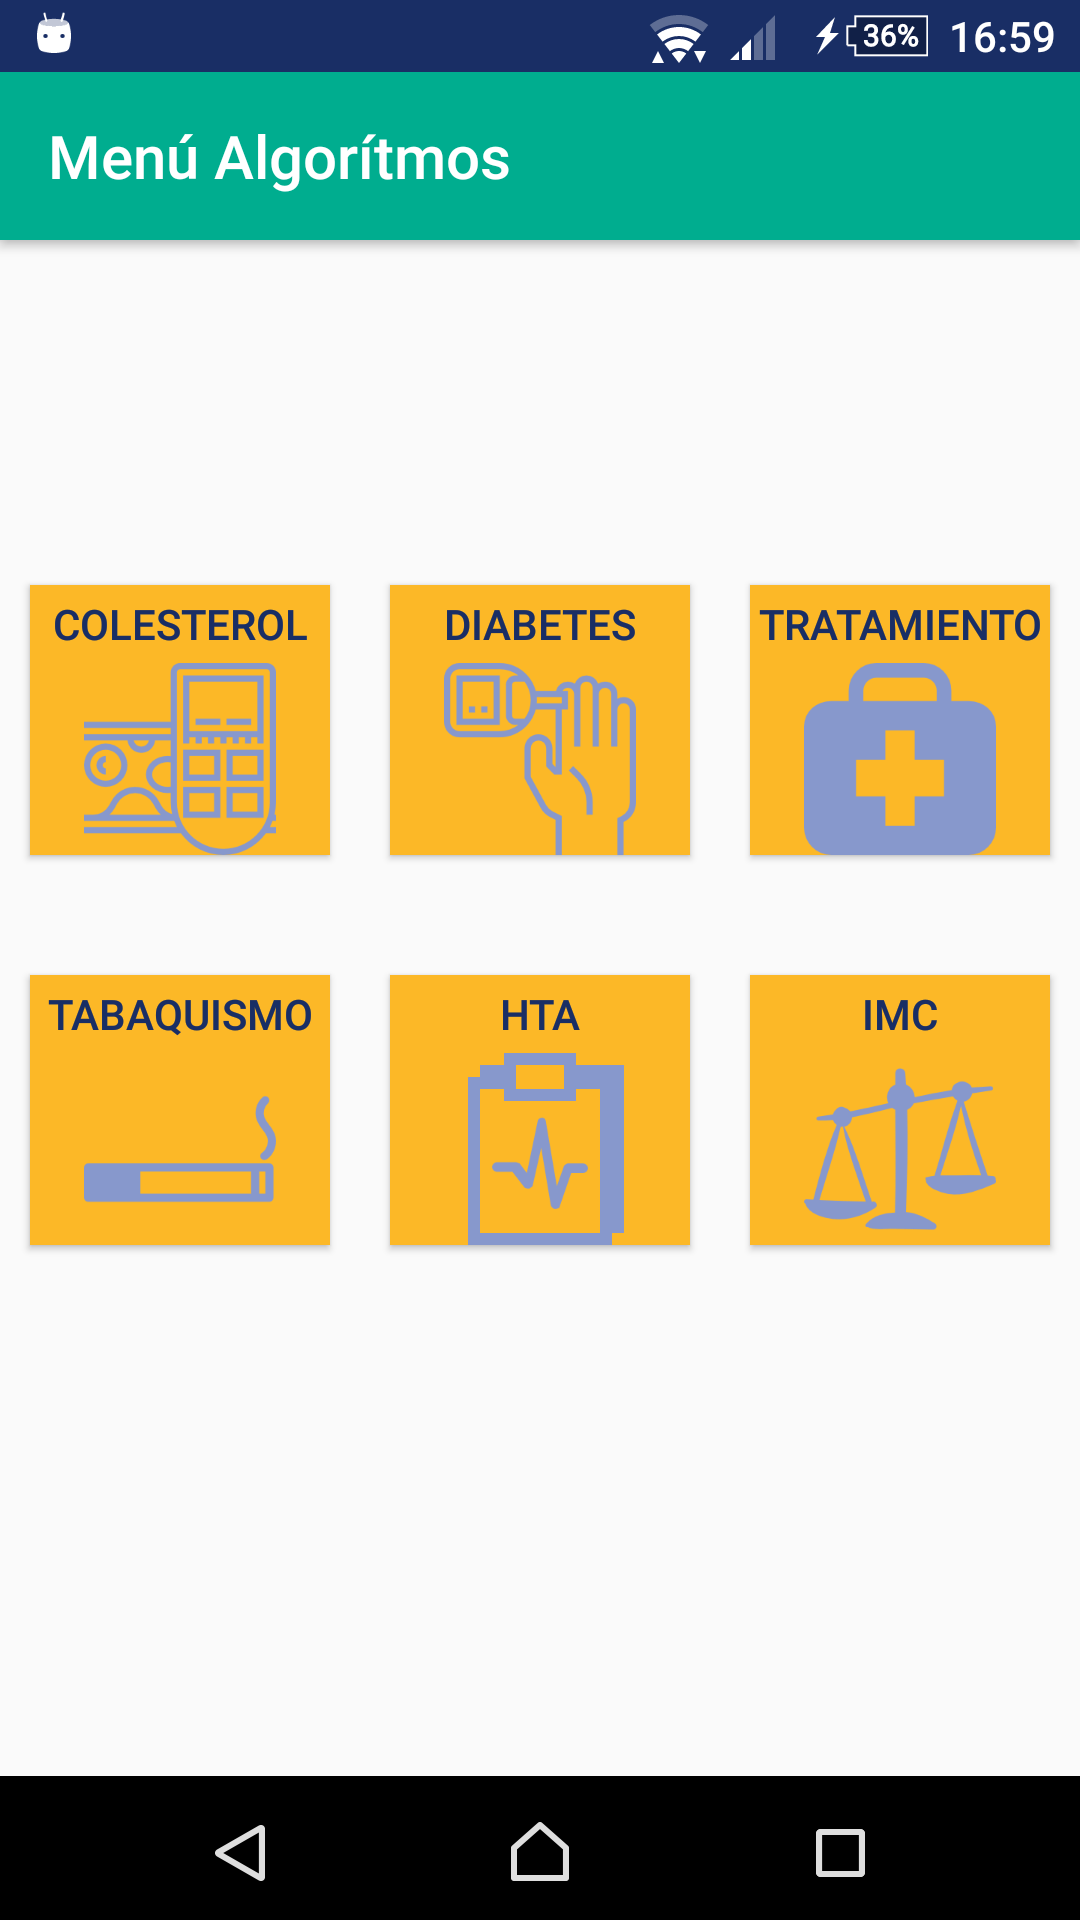
\includegraphics[height= 7cm]{capturas/algoritmos.png}
\caption{Ventana - Consultar Algorítmos}
\end{figure}

\begin{figure}[H]
\centering
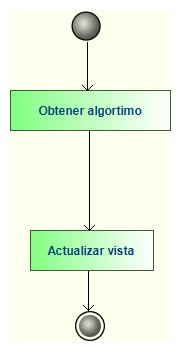
\includegraphics[height= 7cm]{diagramas/ConsultaralgoritmoActivitydiagram.png}
\caption{Diagrama de actividad -  Consultar Algorítmos}
\end{figure}

%CONSULTAR FARMACOS
\subsection {Consultar fármacos}

El profesional accede a una base de datos exterior a la aplicación (\url {http://www.vademecum.es/medicamentos-a_1}) en la que se pueden consultar todos los medicamentos a considerar. Esta es ampliamente utilizada entre el personal sanitario, por lo que podemos confiar que se mantendrá actualizada con frecuencia.

En un principio la idea original era crear nuestra propia base de datos de fármacos, un motor de búsqueda asociado y otras funcionalidades relativas a esta categoría. Sin embargo, tras estudiarlo concluimos que la carga en la aplicación no era algo que nos pudiéramos permitir en una aplicación de esta naturaleza. Todo esto nos llevó a modificar nuestros planes originales y ofrecer el servicio por medio de esta herramienta auxiliar.

\begin{figure}[H]
\centering
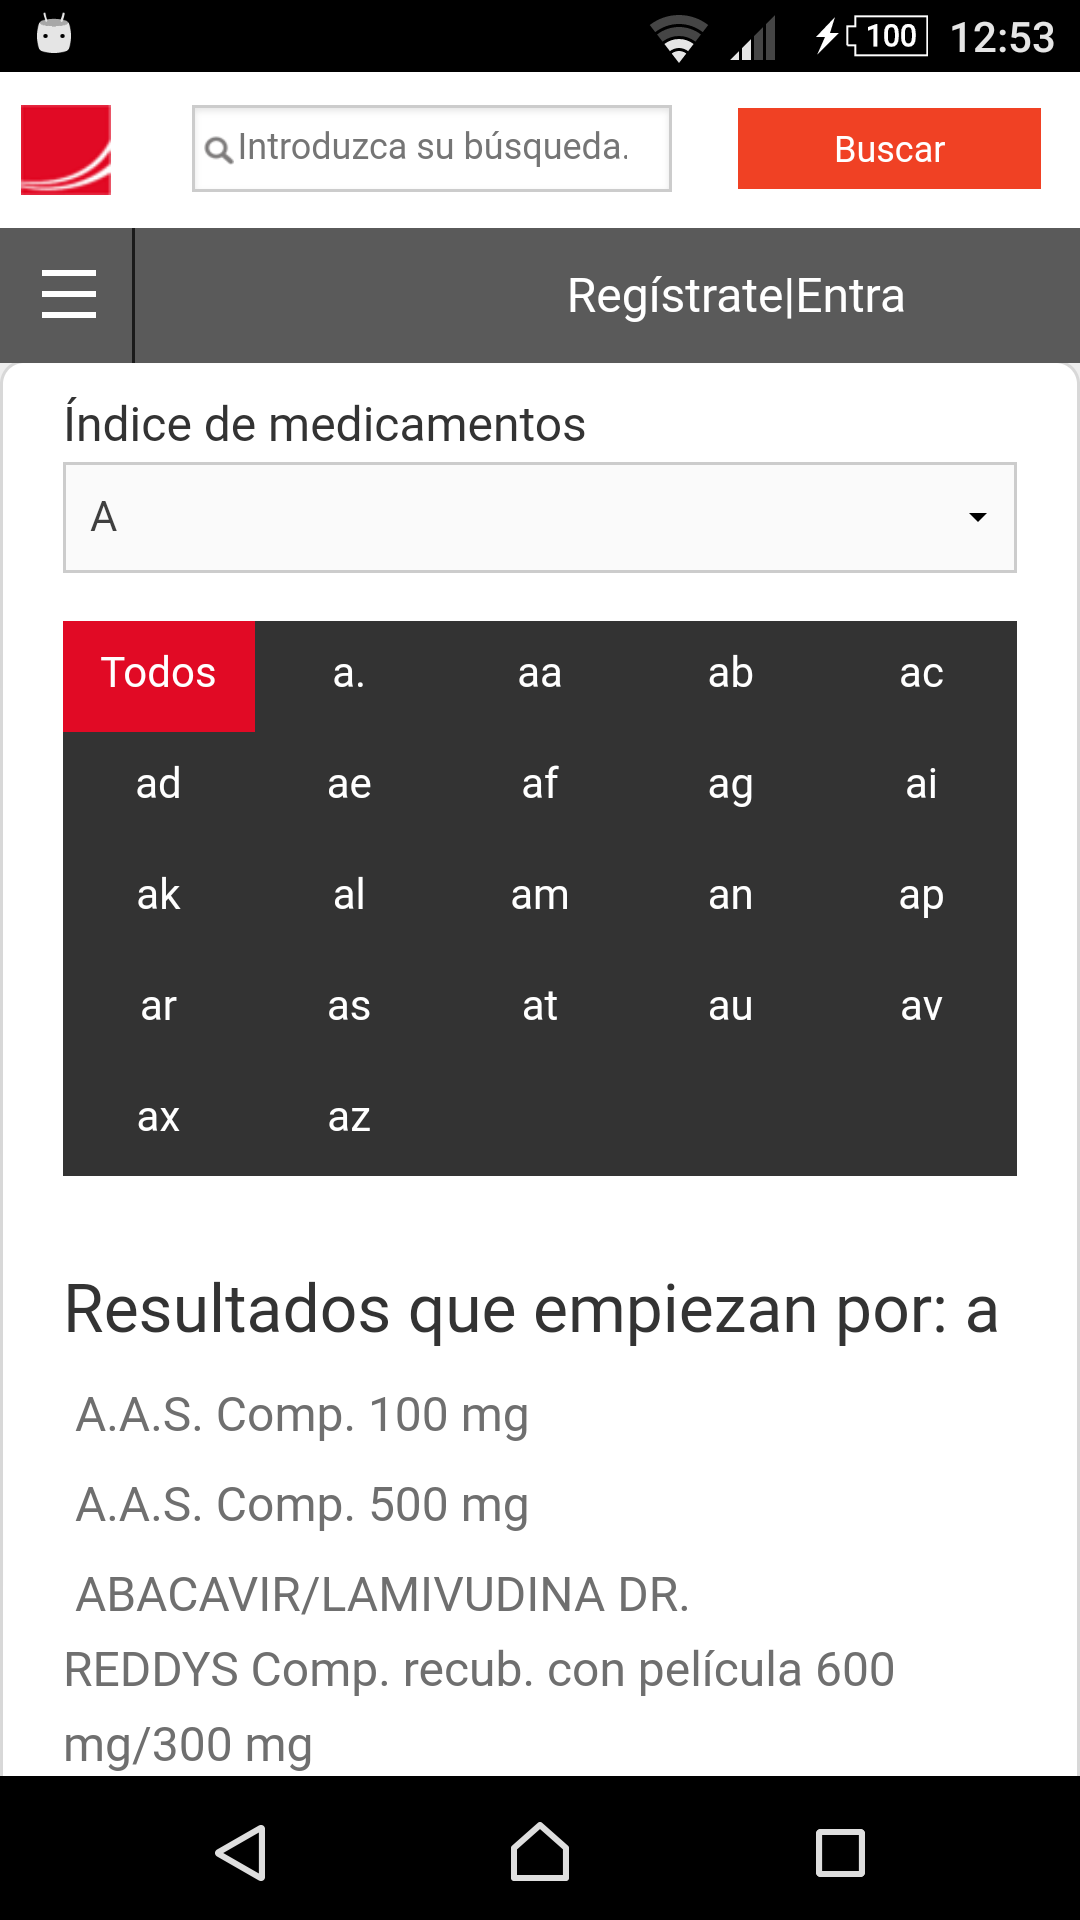
\includegraphics[height= 7cm]{capturas/farmacos.png}
\caption{Ventana - Consultar Fármacos}
\end{figure}

\begin{figure}[H]
\centering
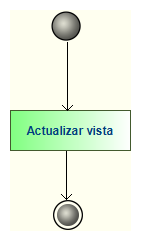
\includegraphics[height= 6cm]{diagramas/ConsultarfarmacosActivitydiagram.png}
\caption{Diagrama de actividad -  Consultar Fármacos}
\end{figure}

%MI PERFIL
\subsection {Mi perfil}

Es imprescindible que el usuario tenga poder administrativo sobre sus propios datos. La causa es que es habitual que el individuo necesite modificar alguno de ellos; ya sea por haber errado en la introducción de la información durante el registro, desear modificar su correo electrónico o querer actualizar su contraseña con frecuencia.

\begin{figure}[H]
\centering
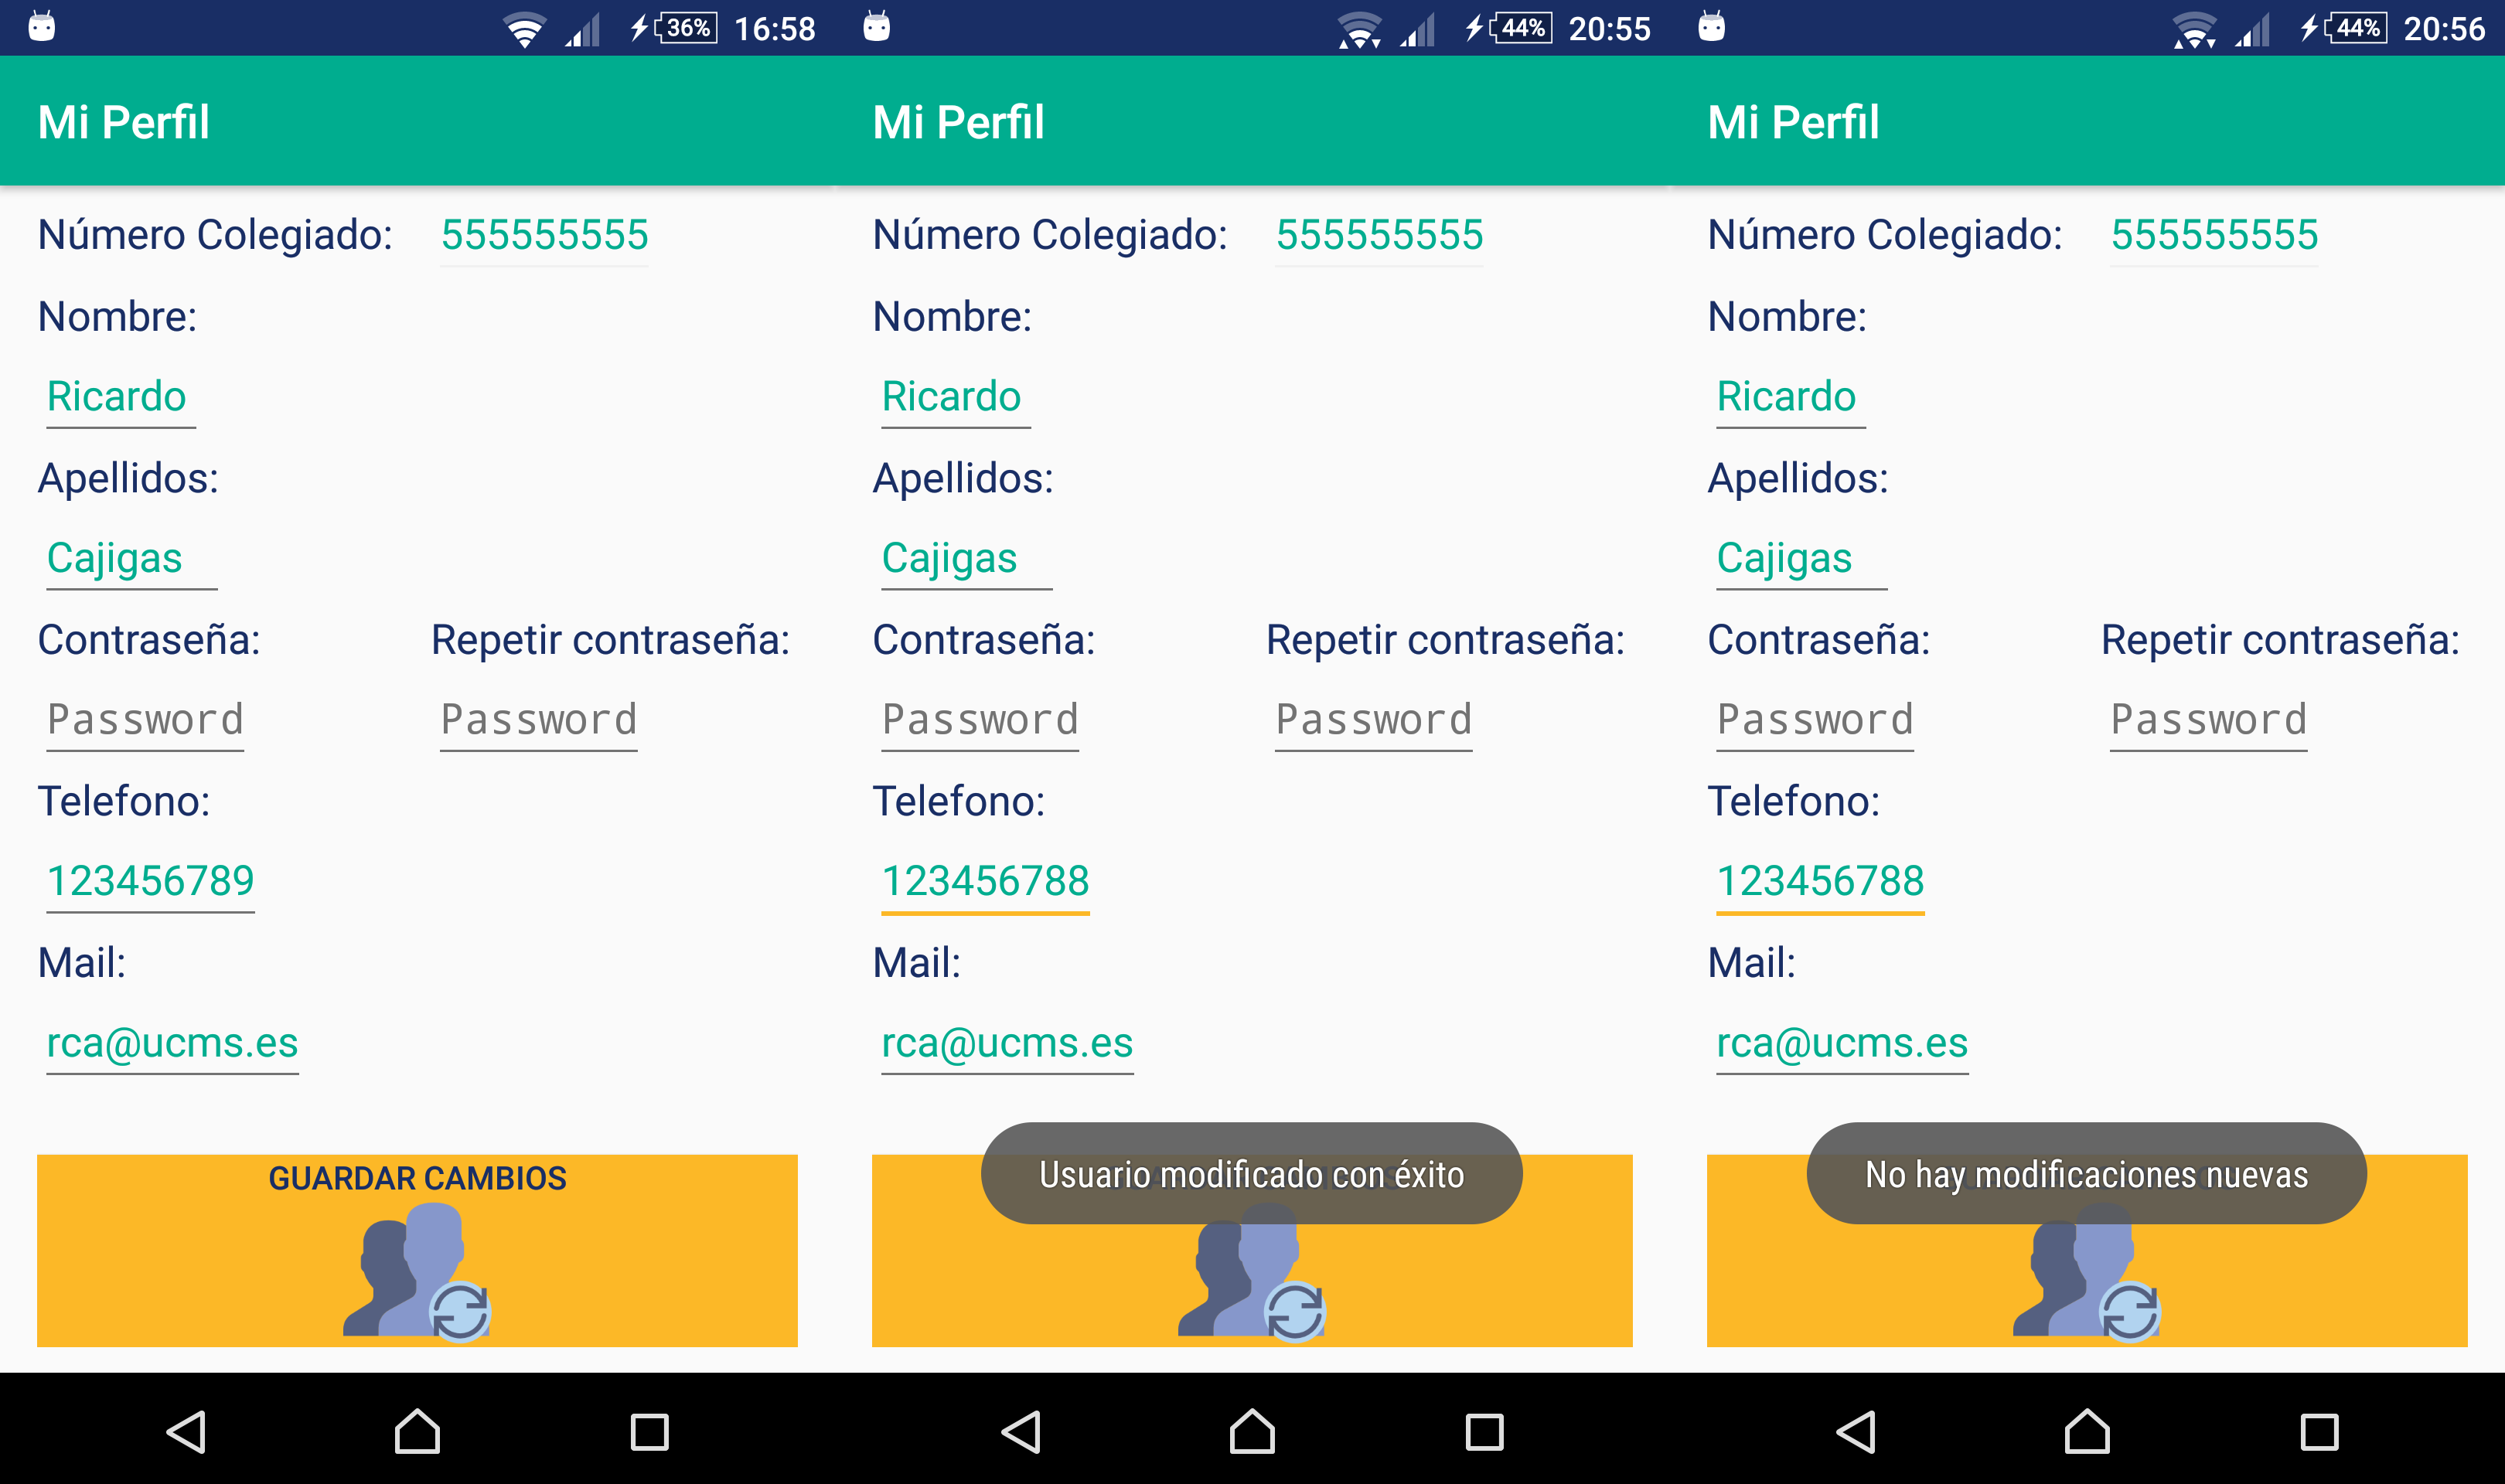
\includegraphics[height= 9cm]{capturas/mi_perfilFull.png}
\caption{Ventana - Mi Perfil}
\end{figure}

\begin{figure}[H]
\centering
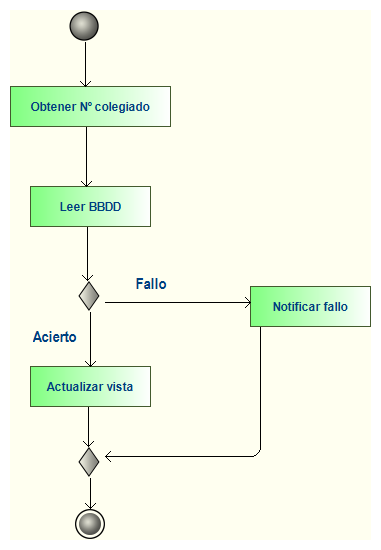
\includegraphics[height= 11cm]{diagramas/VerperfilActivitydiagram.png}
\caption{Diagrama de actividad -  Mi Perfil}
\end{figure}

%%%%%%%%%%%%ADMINISTRADOR
\section {Potestades asignadas al administrador}
La necesidad de gestionar el perfil anterior es esencial incluir un rol administrativo. Este supervisor decidirá la autenticidad de la información suministrada en los registros (Validar/Rechazar aspirante), asi como enmendar posibles errores al proveer o modificar las credenciales y atribuciones de los pacientes.

A continuación estas aptitudes quedan reflejadas en un diagrama.

\begin{figure}[H]
\centering
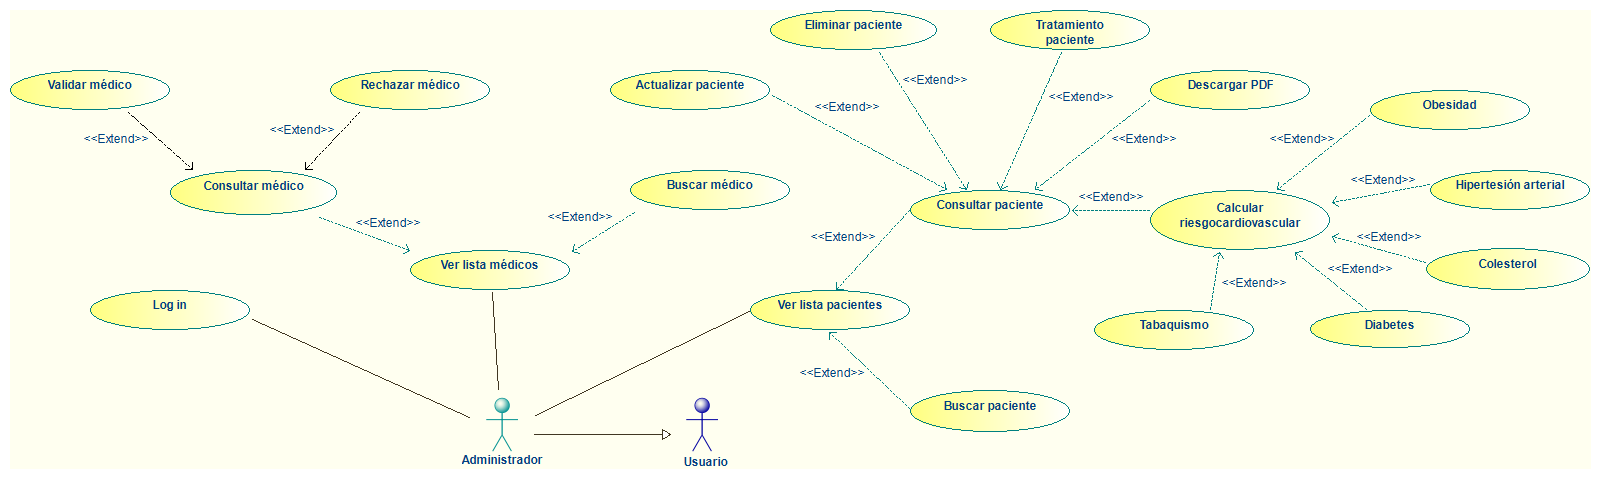
\includegraphics[height= 4.5cm]{diagramas/AdministradorUseCasediagram.png}
\caption{Diagrama de caso de uso - Administrador}
\end{figure}

%LISTA ASPIRANTES
\subsection {Lista de aspirantes}

Como consecuencia de la necesidad de verificar si el canditato realmente posee una identidad como profesional sanitario, se concretó esta funcionalidad con el fin de atender a este dilema. Se introduce el rol de administrador, el cual tiene jurisdicción para conceder acceso a la aplicación o rechazar al solicitante en función de los datos. Los aspirantes se muestran en este catálogo que identifica a cada elemento con su número de colegiado, nombre y apellidos.

\begin{figure}[H]
\centering
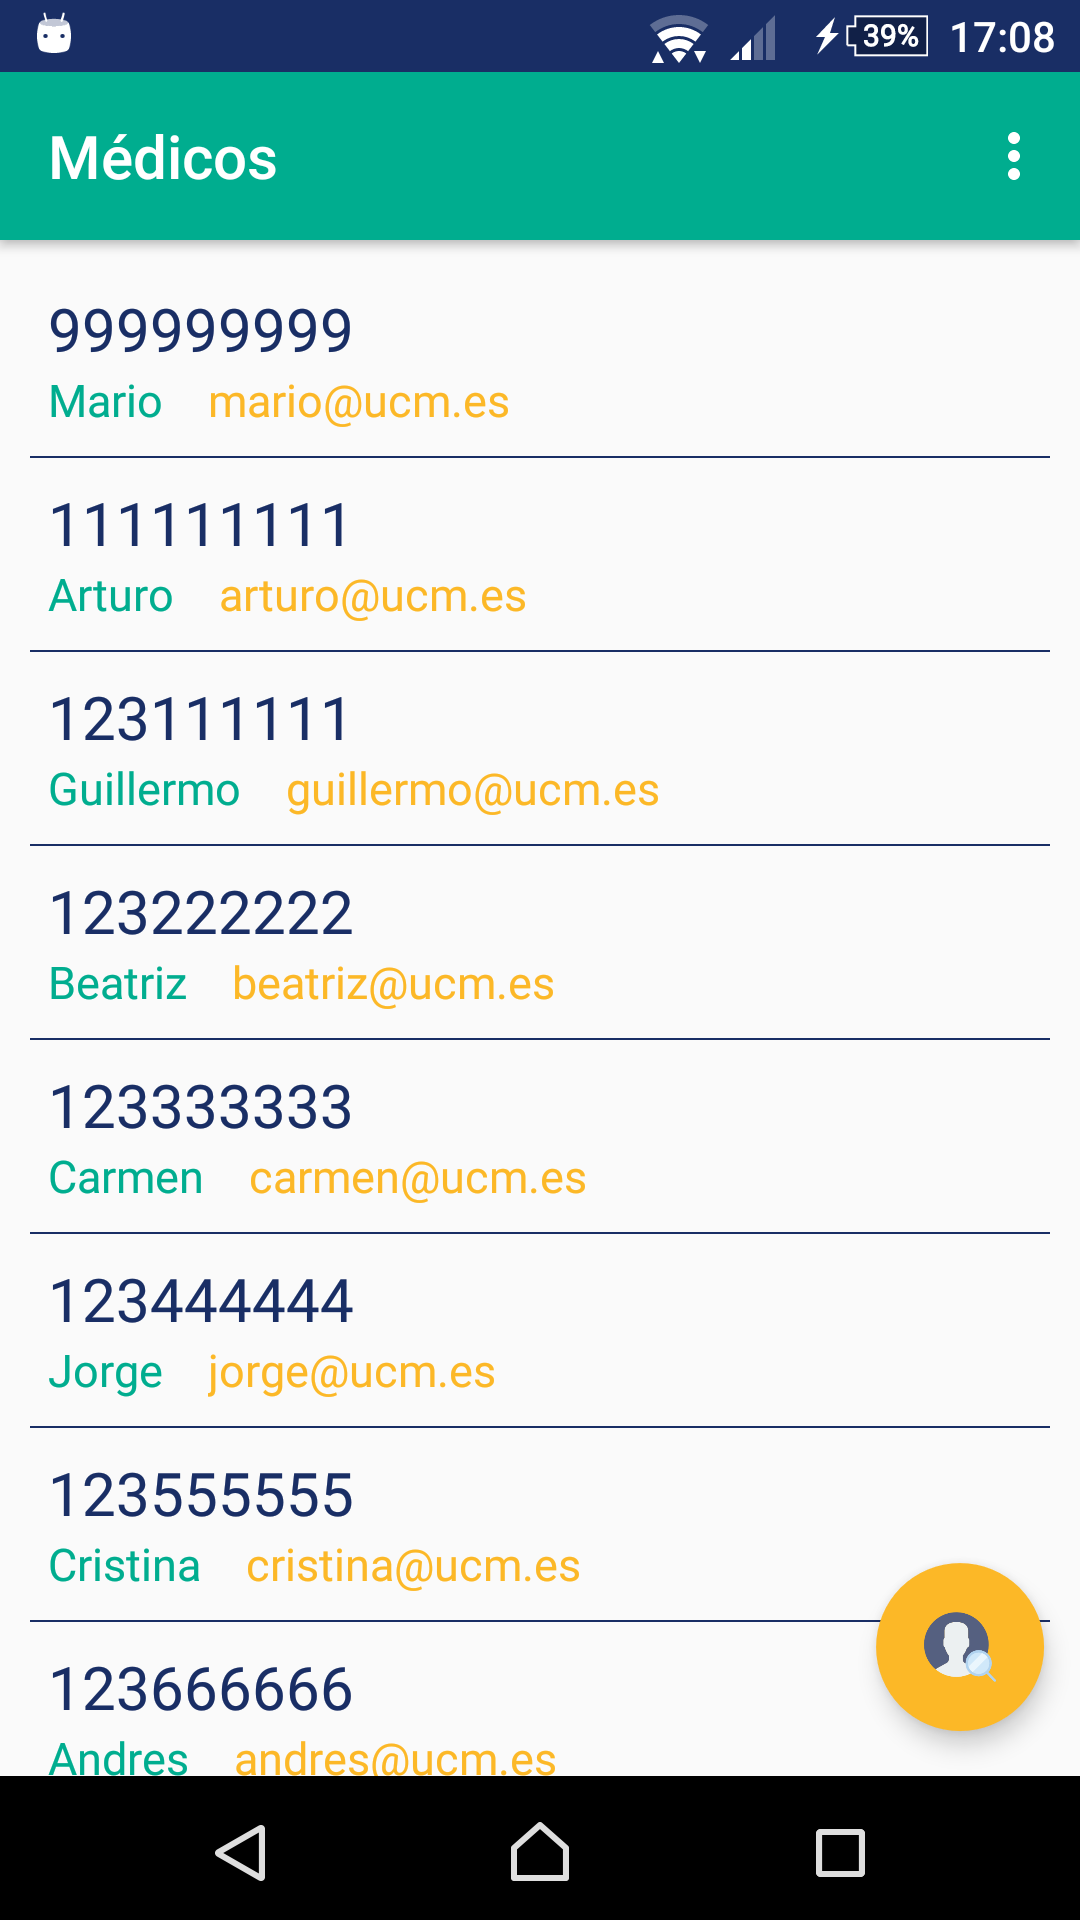
\includegraphics[height= 7cm]{capturas/medicos_lista.png}
\caption{Ventana -  Lista Aspirantes}
\end{figure}

\begin{figure}[H]
\centering
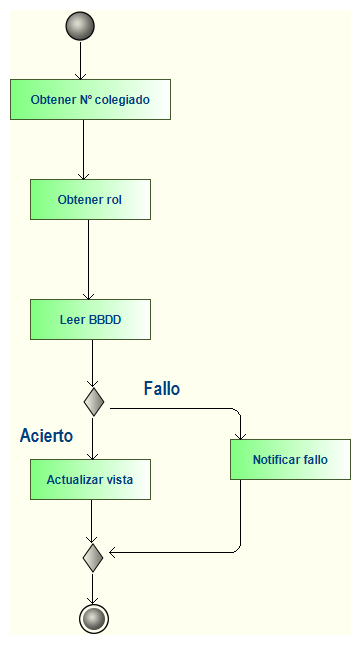
\includegraphics[height= 11cm]{diagramas/ListamedicosActivitydiagram.png}
\caption{Diagrama de actividad -  Lista Aspirantes}
\end{figure}

%BUSCAR ASPIRANTES
\subsection {Buscar aspirante}

En numerosas ocasiones, el supervisor de la aplicación podría requerir localizar a un sujeto en específico. Como solución a este problema se introduce un motor de búsqueda, el cual ofrece filtrar por nombre, número de colegiado, mail y/o una combinación de estos últimos.

\begin{figure}[H]
\centering
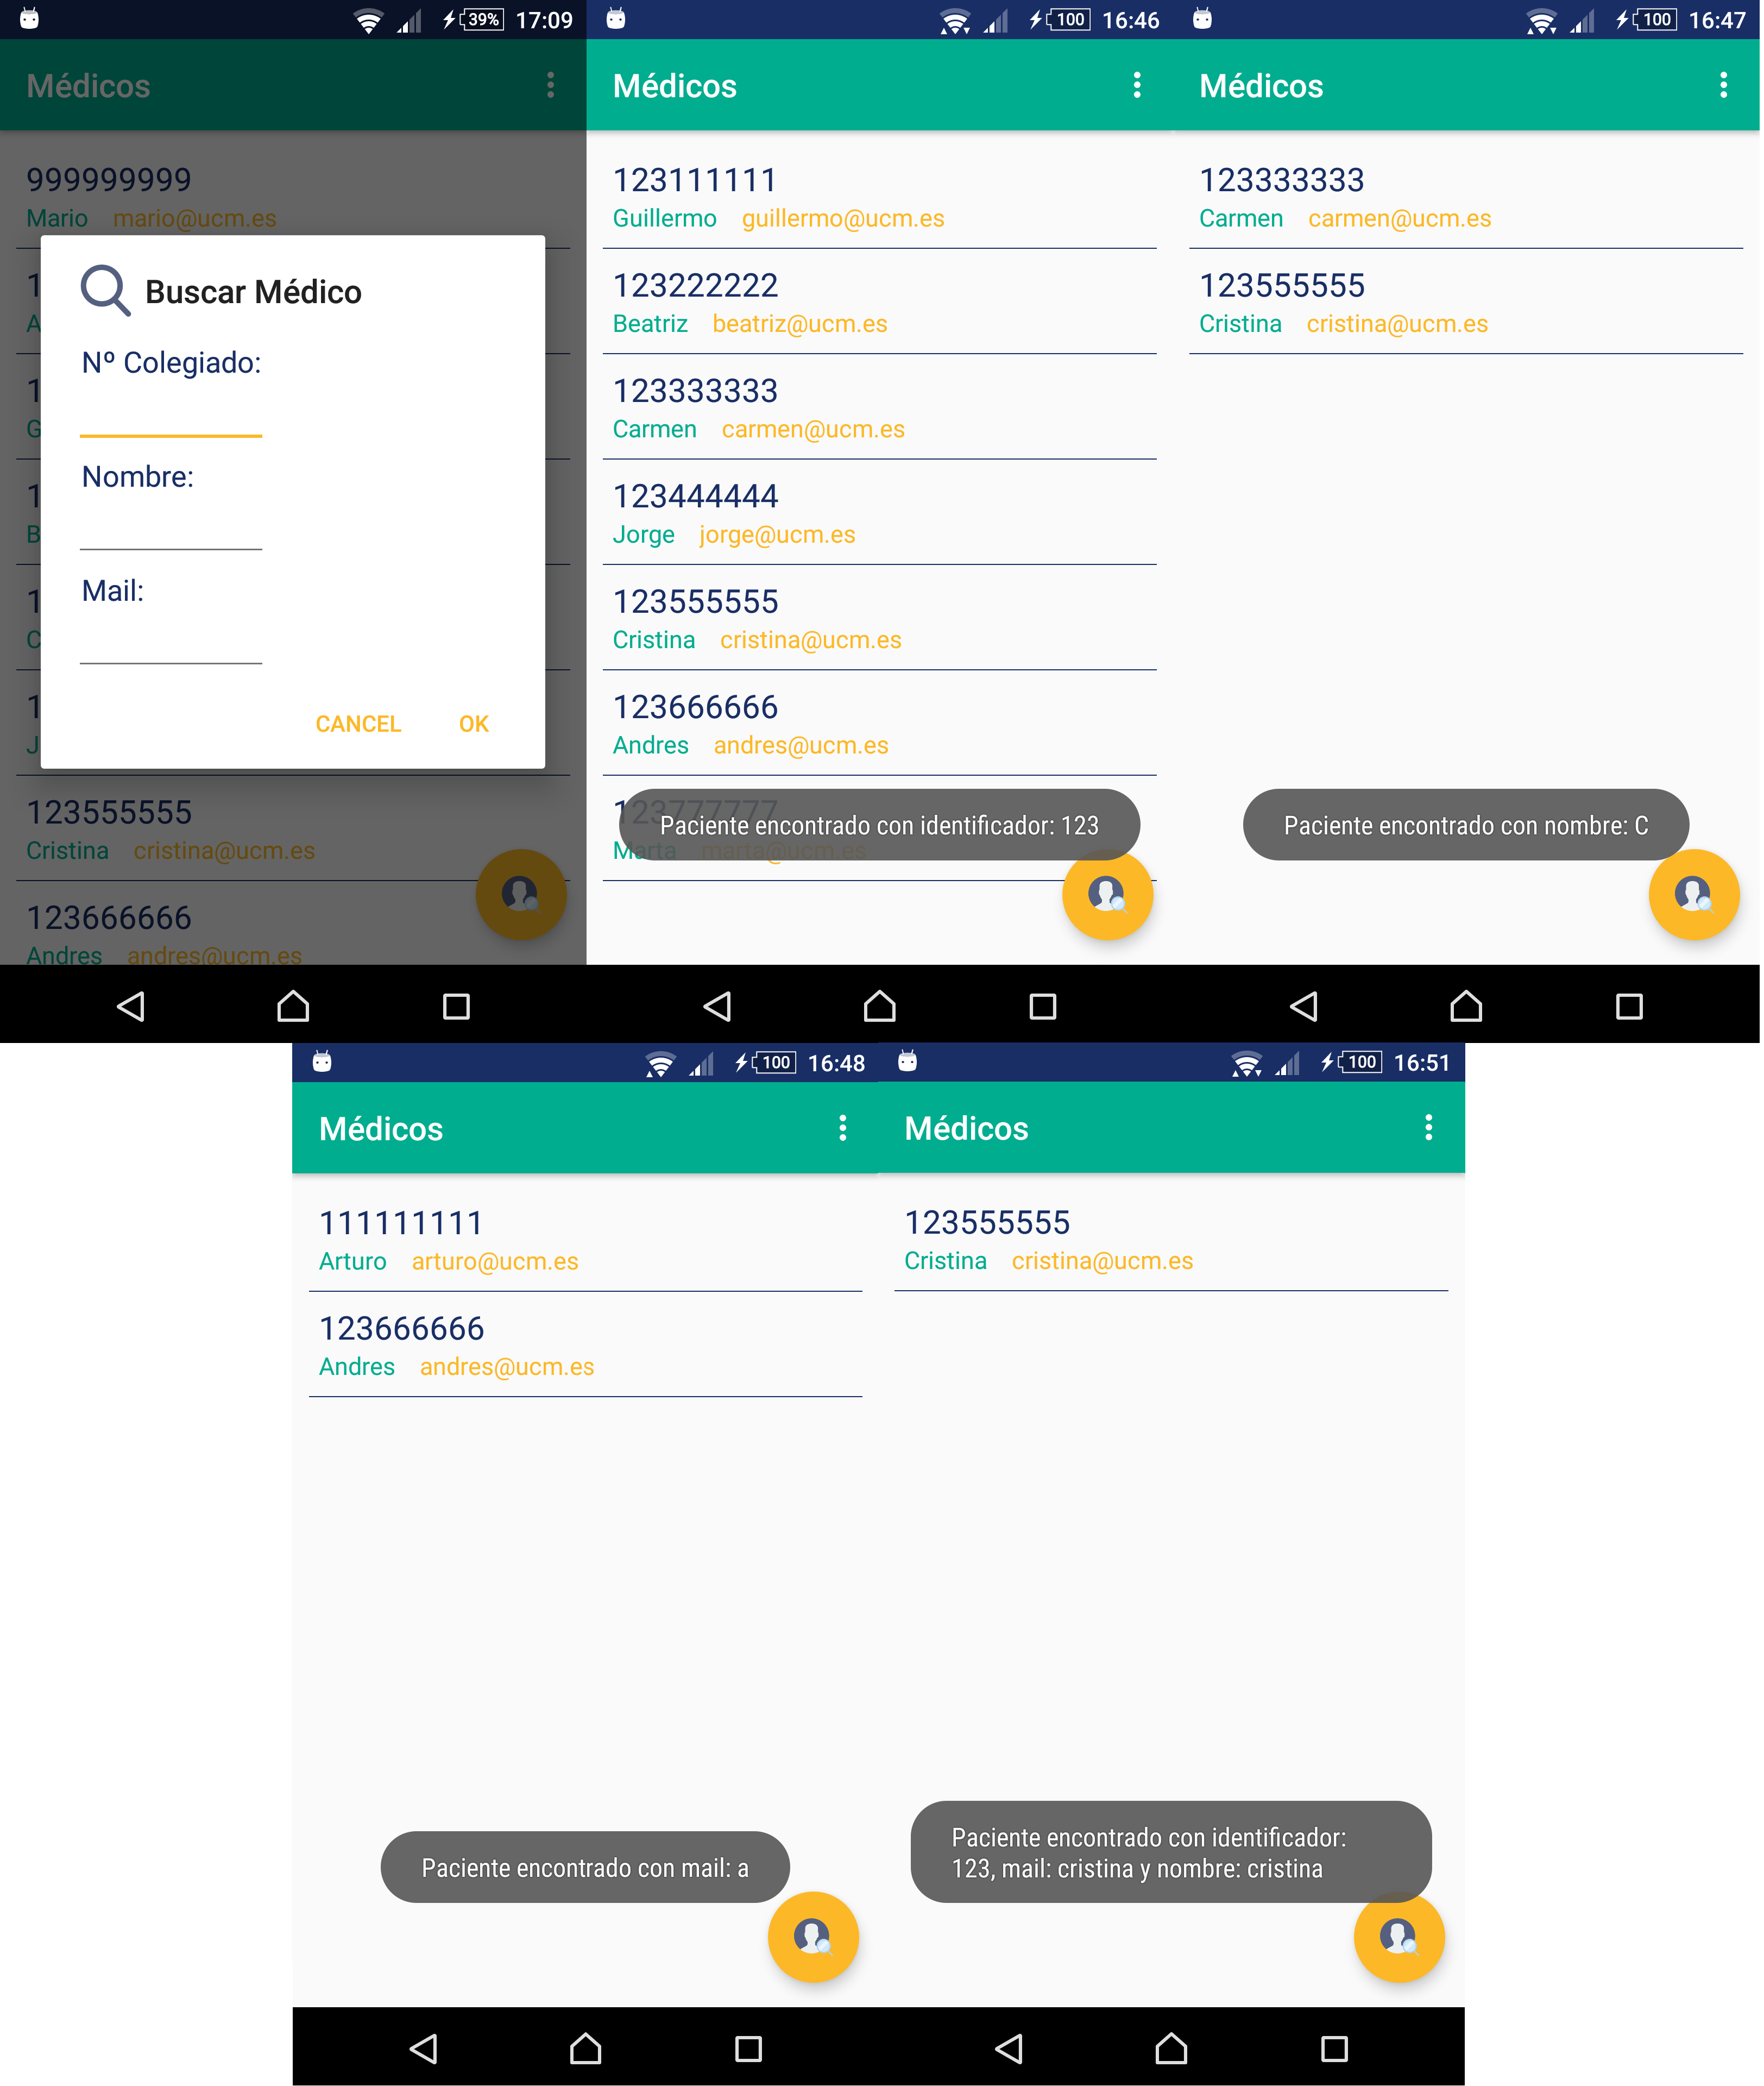
\includegraphics[height= 18cm]{capturas/buscarMedicoFull.png}
\caption{Ventana -  Buscar Aspirante}
\end{figure}

\begin{figure}[H]
\centering
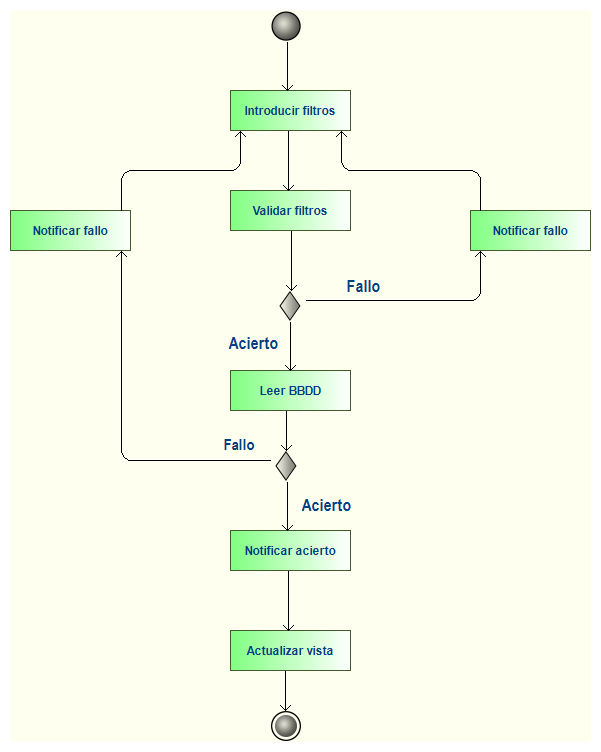
\includegraphics[height= 11cm]{diagramas/BuscarmedicoActivitydiagram.png}
\caption{Diagrama de actividad -  Buscar Aspirante}
\end{figure}

%CONSULTAR ASPIRANTE
\subsection {Consultar aspirante}

Al interactuar con un elemento de la lista de aspirantes, al administrador se le guía a otra ventana donde puede consultar una documentación más detallada sobre el candidato. A través de esta interfaz, el médico podrá finalmente validarle o removerle en función de si sus datos son fidedignos o no. 

\begin{figure}[H]
\centering
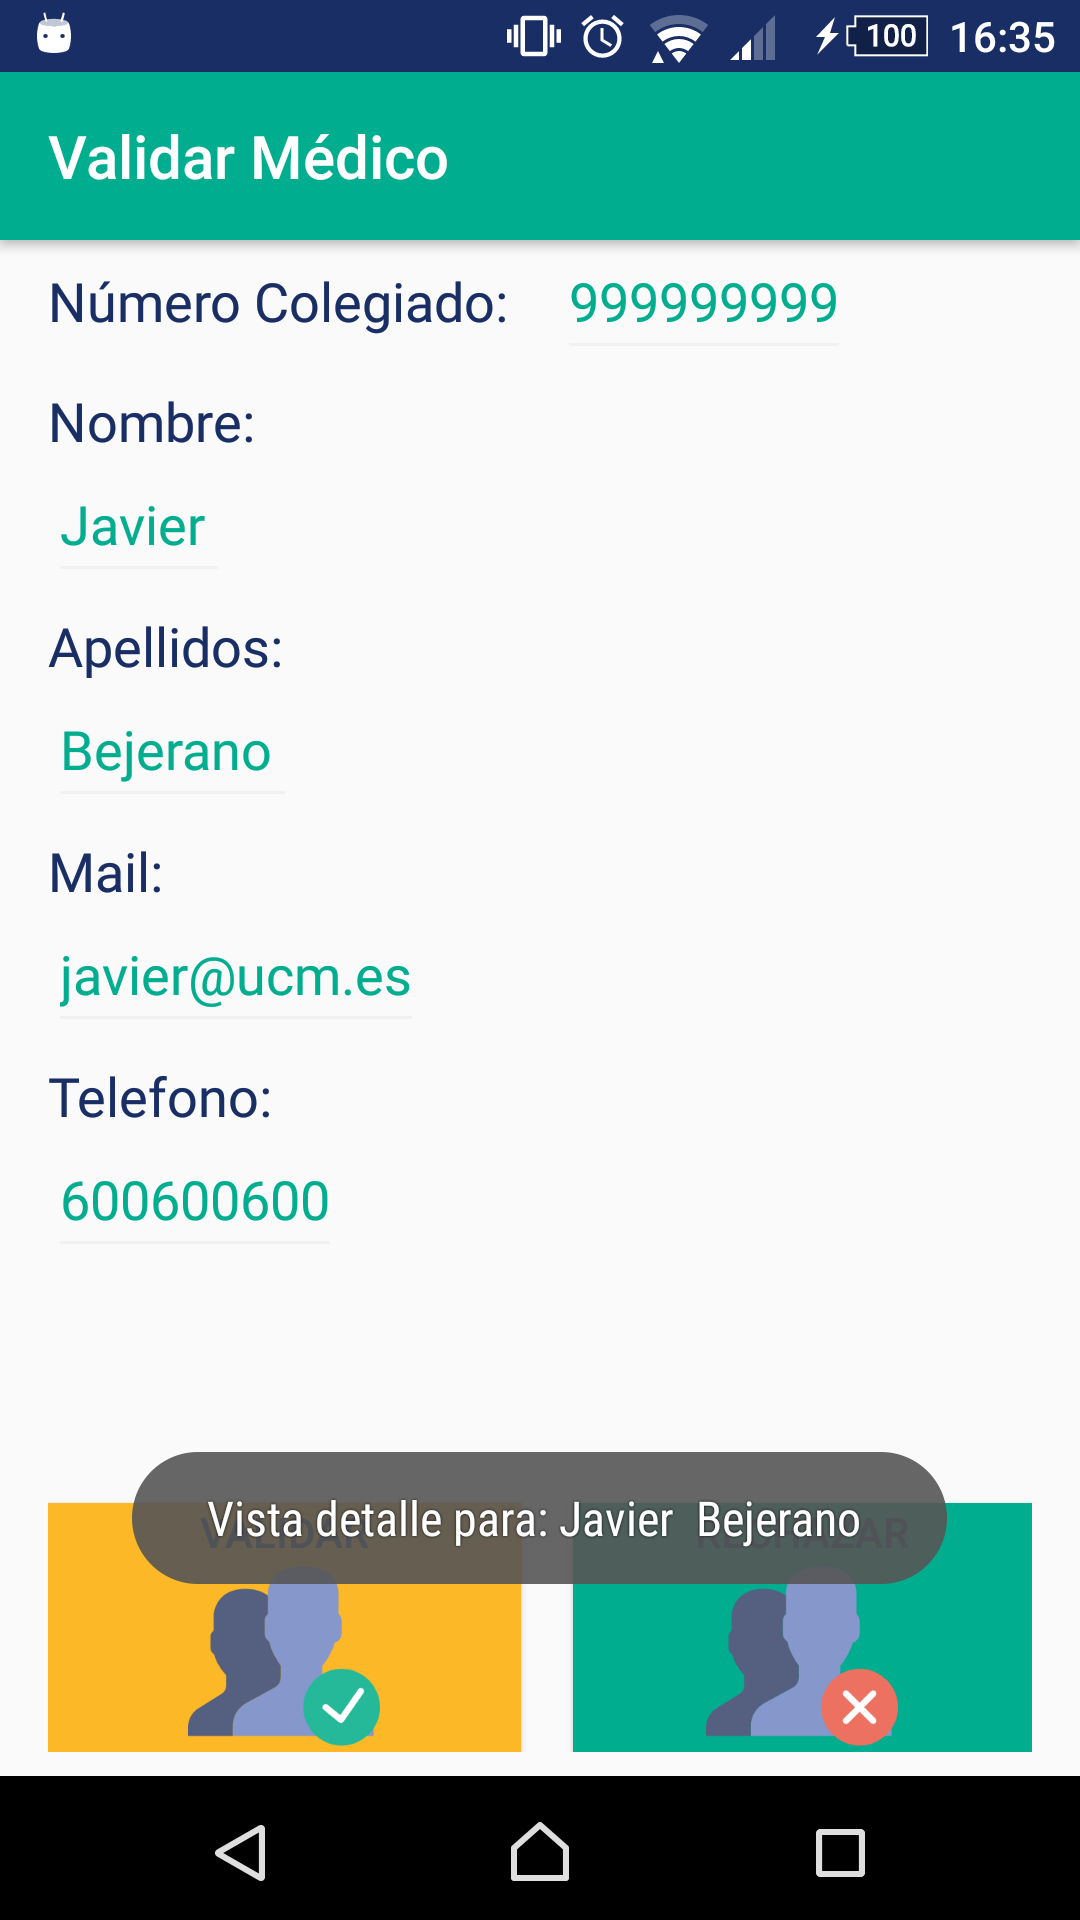
\includegraphics[height= 7cm]{capturas/consultar_medico.png}
\caption{Ventana -  Consultar Aspirante}
\end{figure}

\begin{figure}[H]
\centering
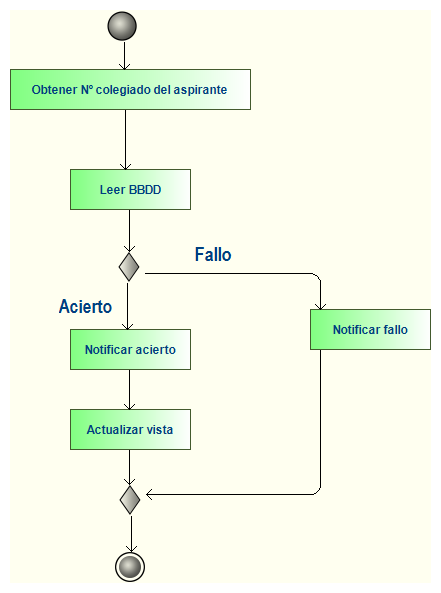
\includegraphics[height= 11cm]{diagramas/ConsultarmedicoActivitydiagram.png}
\caption{Diagrama de actividad -  Consultar Aspirante}
\end{figure}

%VALIDAR ASPIRANTE
\subsection {Validar aspirante}

Si el usuario presiona el botón de validar en la ventana mencionada anteriormente el sujeto evaluado será confirmado como un profesional verídico y será registrado como un auténtico médico en la aplicación. A partir de este momento, el solicitante podrá acceder a su cuenta e interactuar con lo que ofrece la app. 

\begin{figure}[H]
\centering
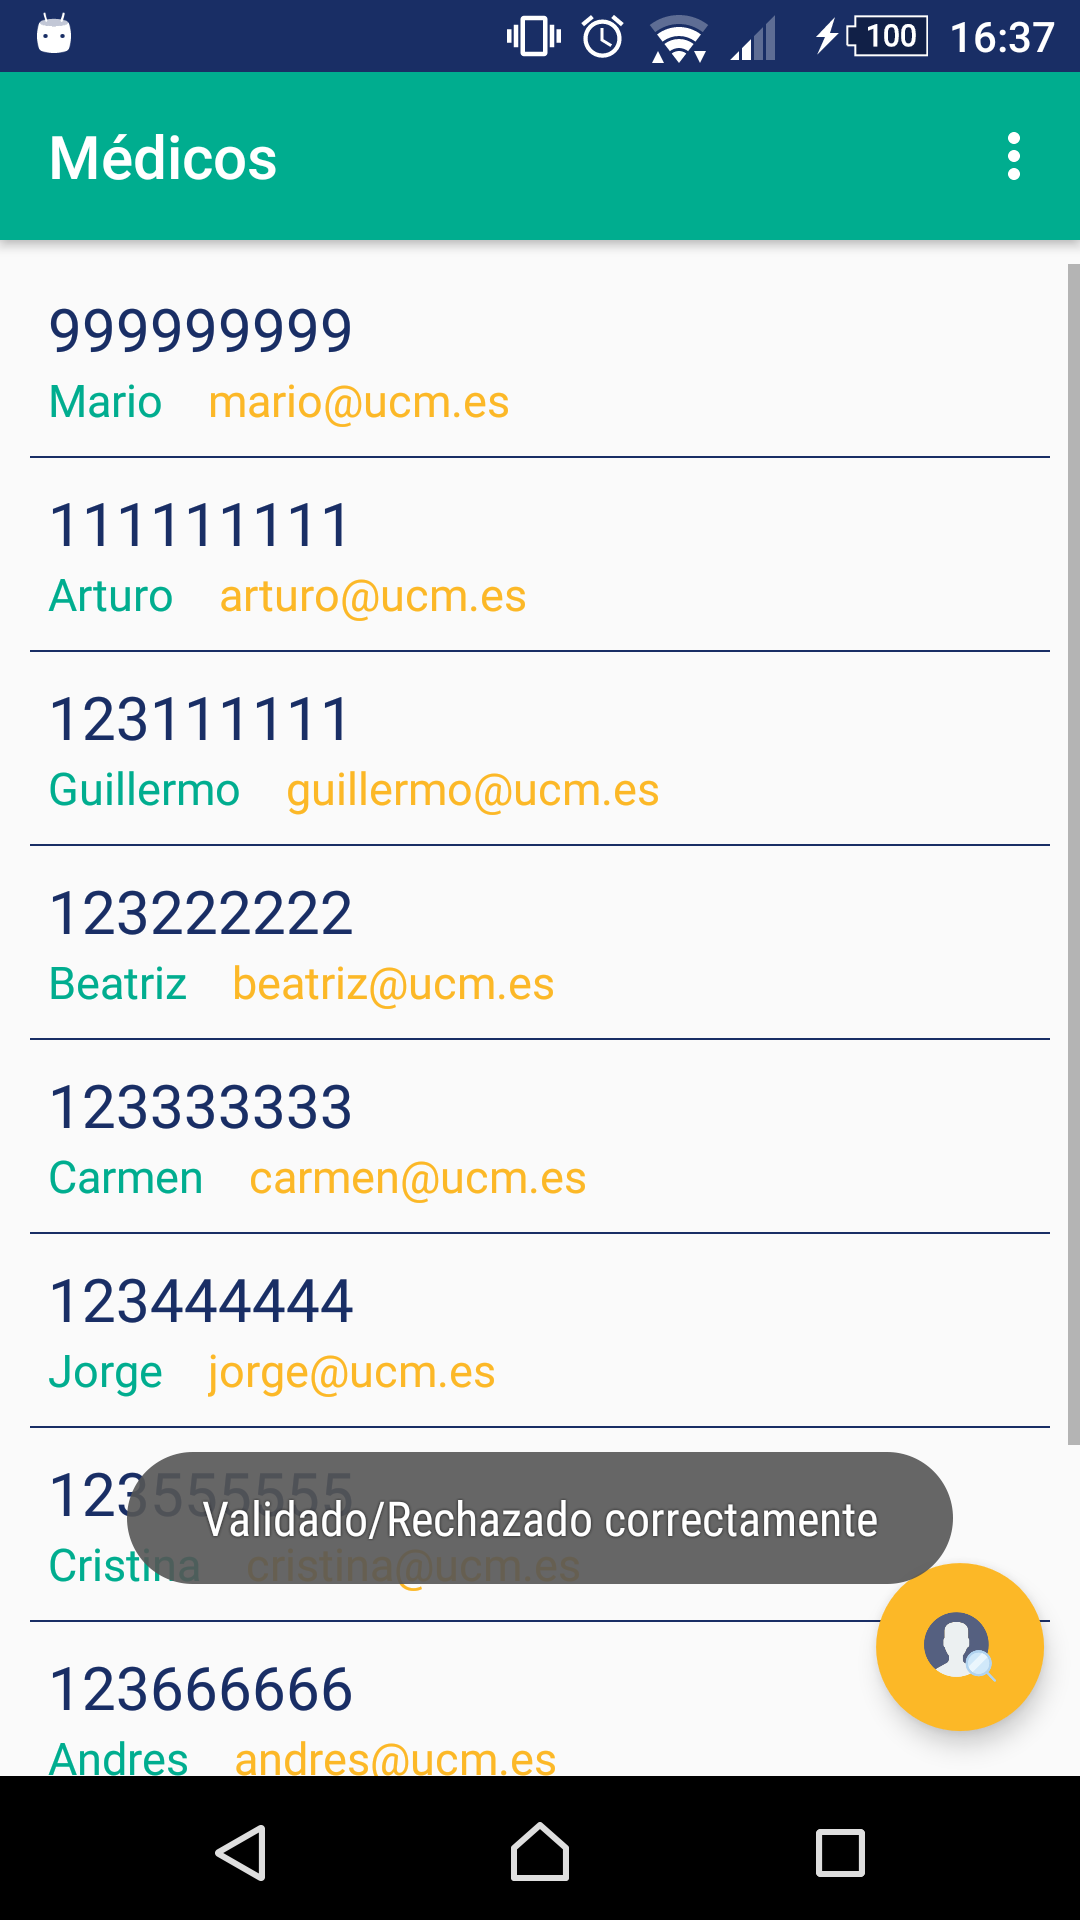
\includegraphics[height= 7cm]{capturas/validar_medico.png}
\caption{Ventana -  Validar Aspirante}
\end{figure}

\begin{figure}[H]
\centering
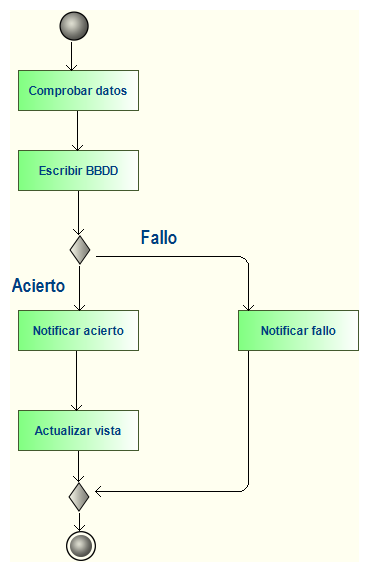
\includegraphics[height= 11cm]{diagramas/ValidarmedicoActivitydiagram.png}
\caption{Diagrama de actividad -  Validar Aspirante}
\end{figure}

%RECHAZAR ASPIRANTE
\subsection {Rechazar aspirante}

Si por el contrario el individuo presiona el botón rechazar, la candidatura actual será revocada y todos los datos relativos a ese registro serán removidos. 

\begin{figure}[H]
\centering
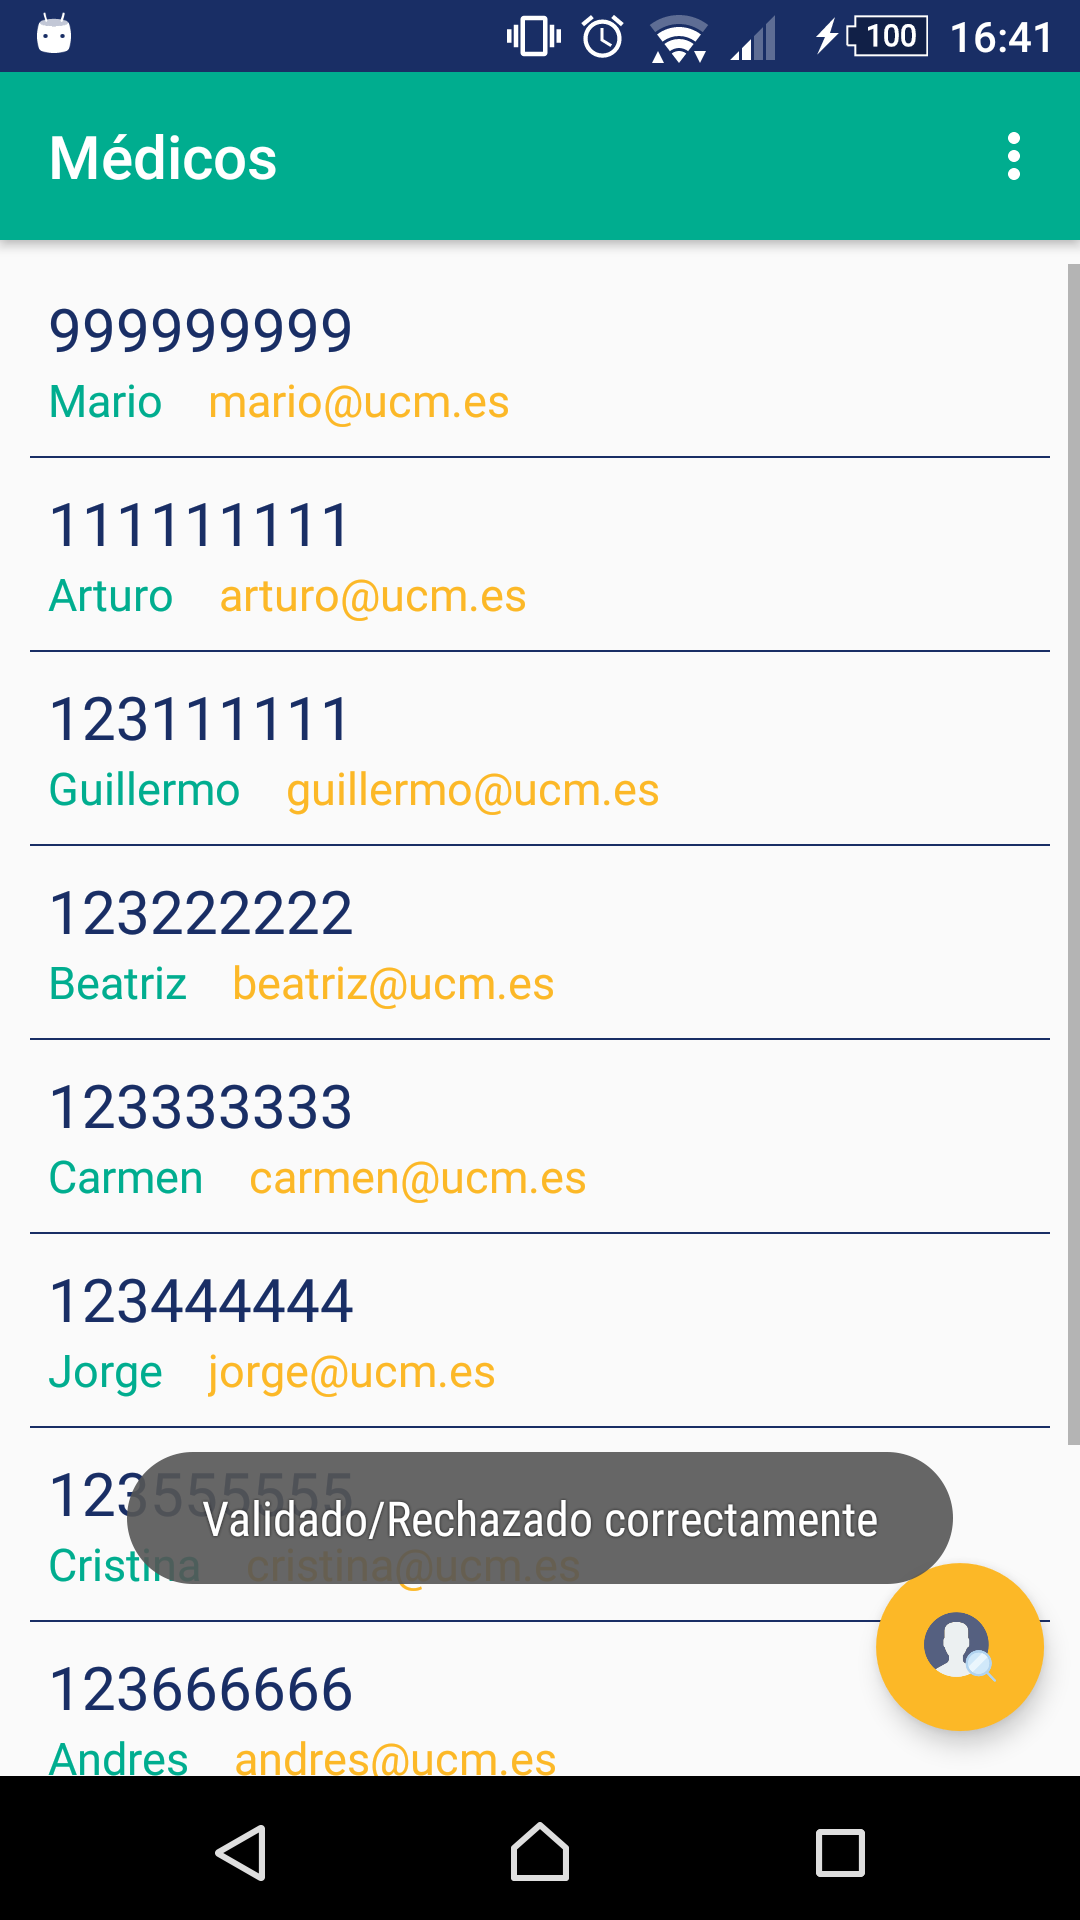
\includegraphics[height= 7cm]{capturas/rechazar_medico.png}
\caption{Ventana -  Rechazar Aspirante}
\end{figure}

\begin{figure}[H]
\centering
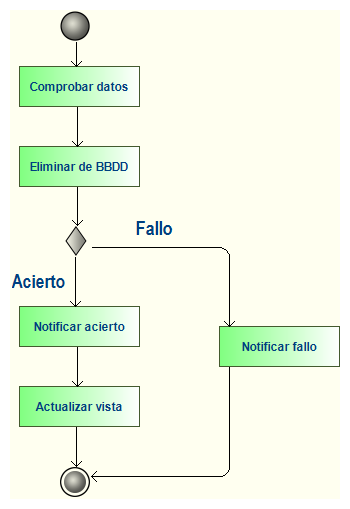
\includegraphics[height= 11cm]{diagramas/RechazarmedicoActivitydiagram.png}
\caption{Diagrama de actividad -  Rechazar Aspirante}
\end{figure}

%%%%%%%%%%%%COMUNES
\section {Facultades comunes a ambos perfiles}

Existen situaciones compartidas por ambos prototipos de usuario. En la app se suceden situaciones generales como la contigencia de que el número de pacientes alcance dimensiones de cierta magnitud concluyendo en un sistema de organización de los mismos, el registro y acceso de los usuarios a su cuenta, y la consulta y alteración de los datos de un paciente.

%INICIO DE SESION
\subsection {Inicio de sesión}

Cuando ejecutamos la aplicación nos aparece el login, el cual nos permite autentificar nuestras credenciales para acceder a nuestra cuenta. Se nos requerirá el número de colegiado y la contraseña.
Si no dispones de una cuenta puedes aplicar por una mediante el botón de la parte inferior. Esta funcionalidad se explica en detalle en el siguiente punto.

\begin{figure}[H]
\centering
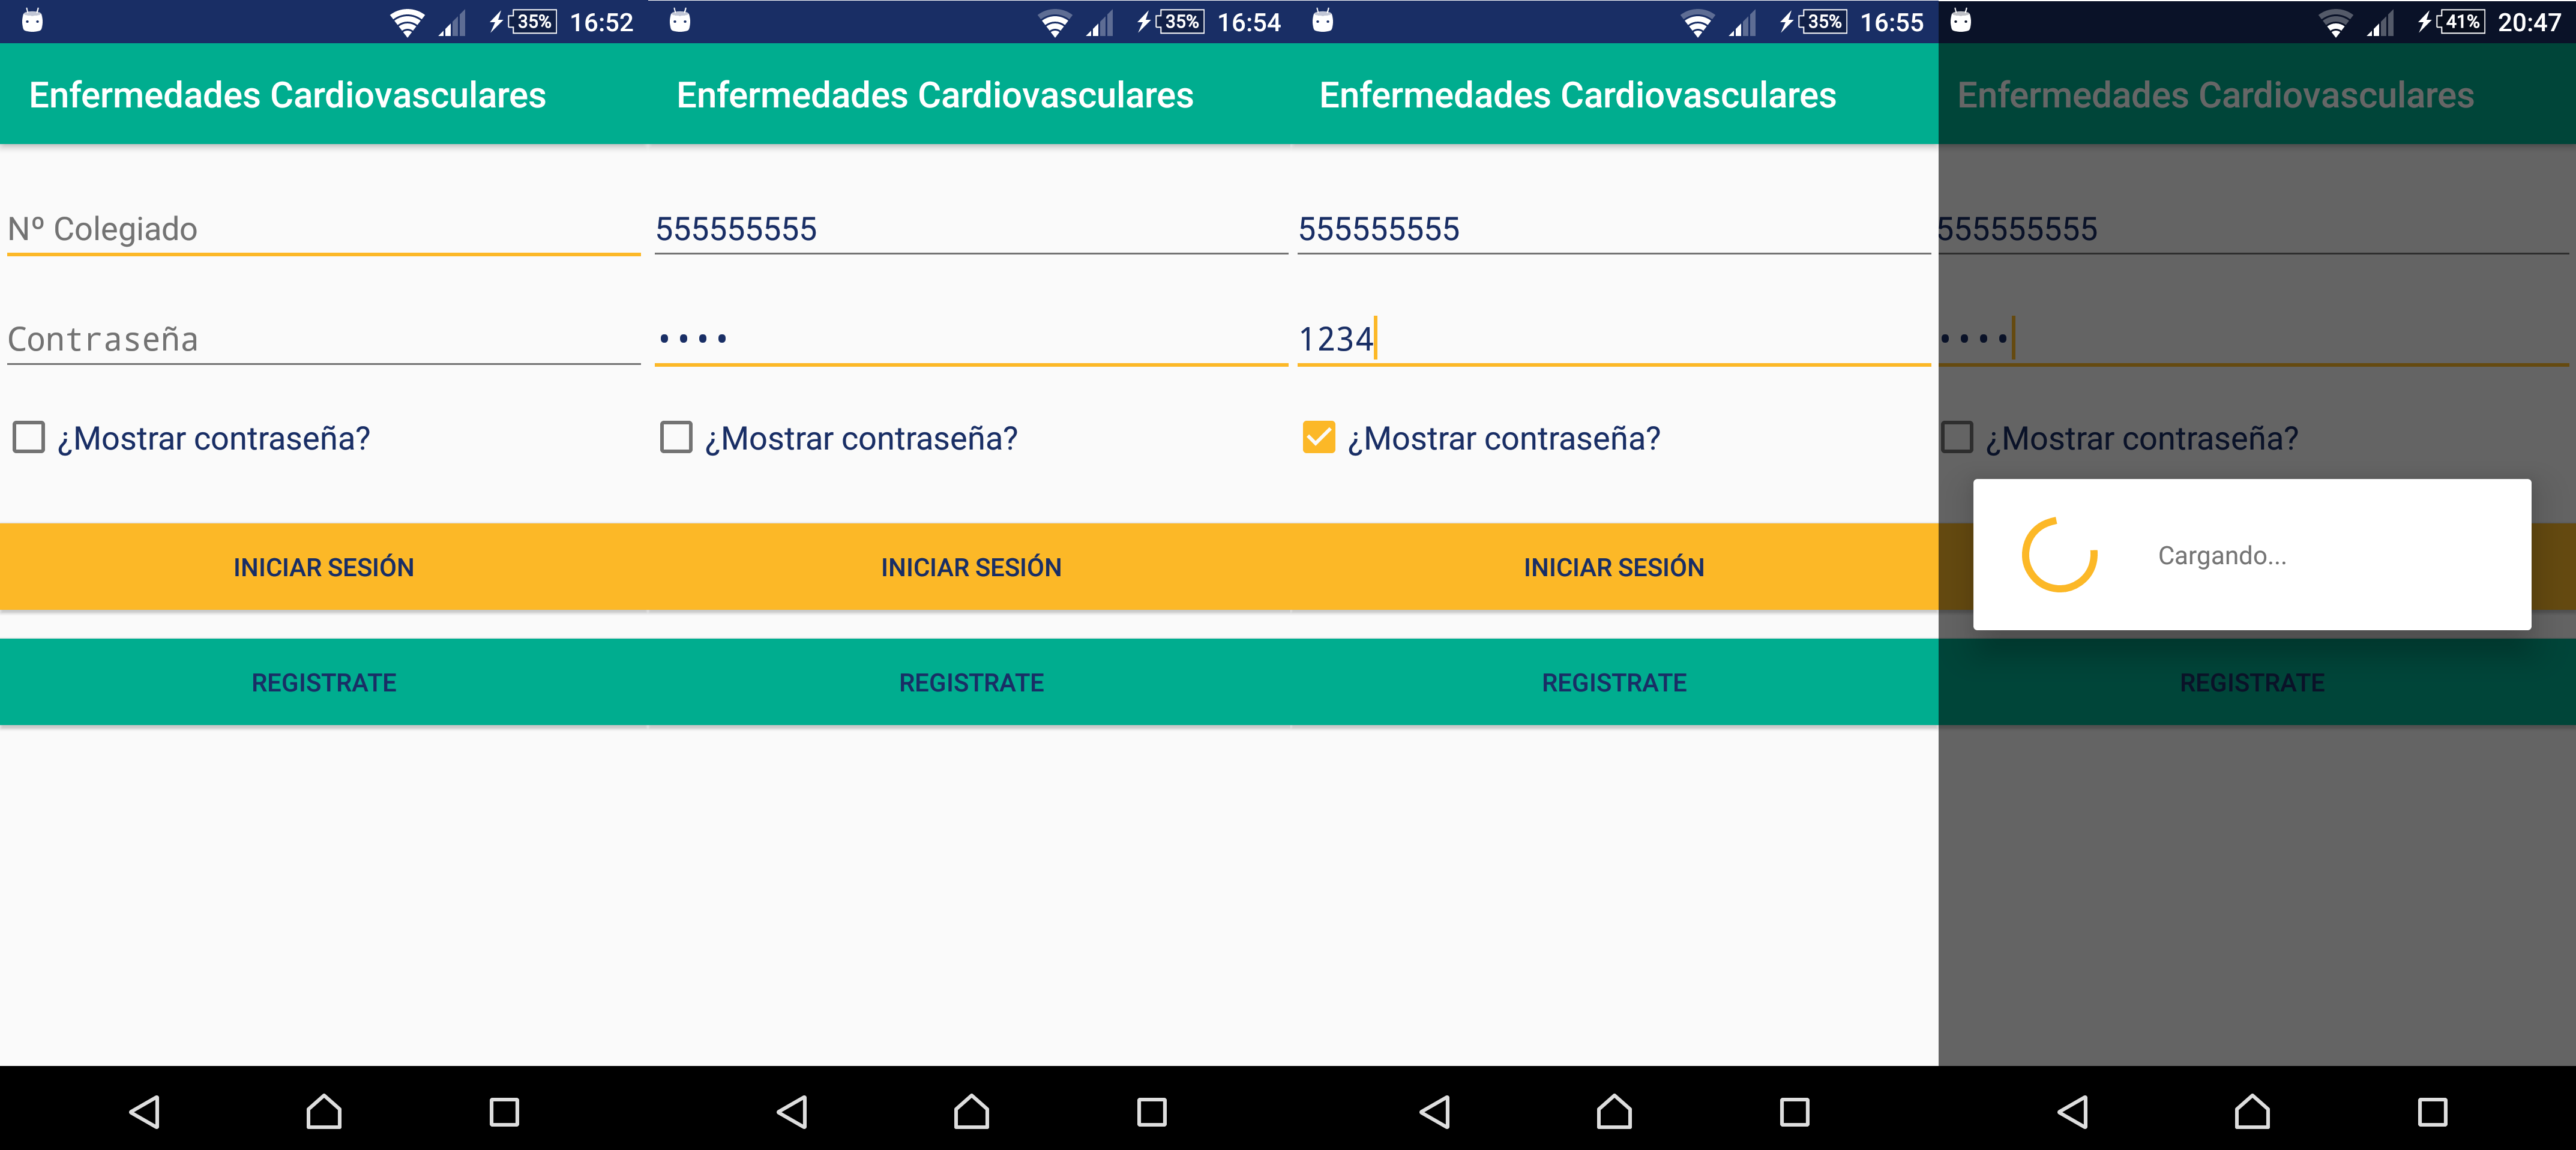
\includegraphics[height=6.7cm]{capturas/logIn.png}
\caption{Ventana - Inicio de sesión}
\end{figure}

\begin{figure}[H]
\centering
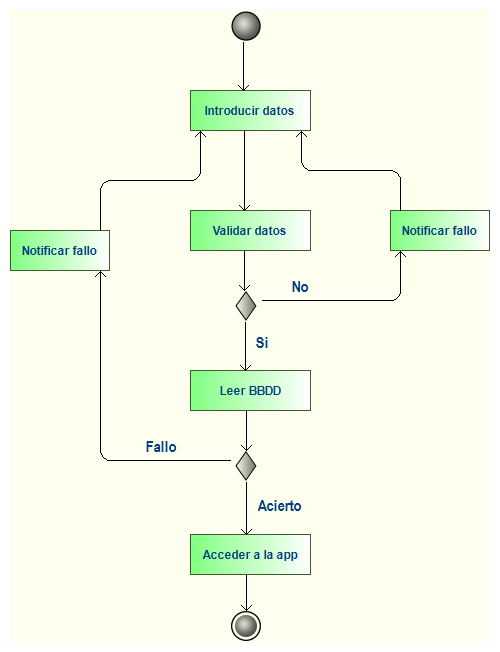
\includegraphics[height= 11cm]{diagramas/LoginActivitydiagram.png}
\caption{Diagrama de actividad - Inicio Sesión}
\end{figure}

%REGISTRO
\subsection {Registro}

Si el solicitante desea adquirir una cuenta como médico pueden introducir sus datos en esta ventana. La aplicación requiere el nombre y apellidos, el número de colegiado que identifica al profesional sanitario, la dirección de correo electrónico, el teléfono de contacto y la contraseña que se va utilizar posteriormente para tener acceso a su cuenta en la aplicación. Todos los campos mencionados son obligatorios y se comprobará que los datos introducidos son válidos.
La aplicación notificará el éxito o fracaso de la operación, resaltando los fallos específicos ocurridos en este último caso.

\begin{figure}[H]
\centering
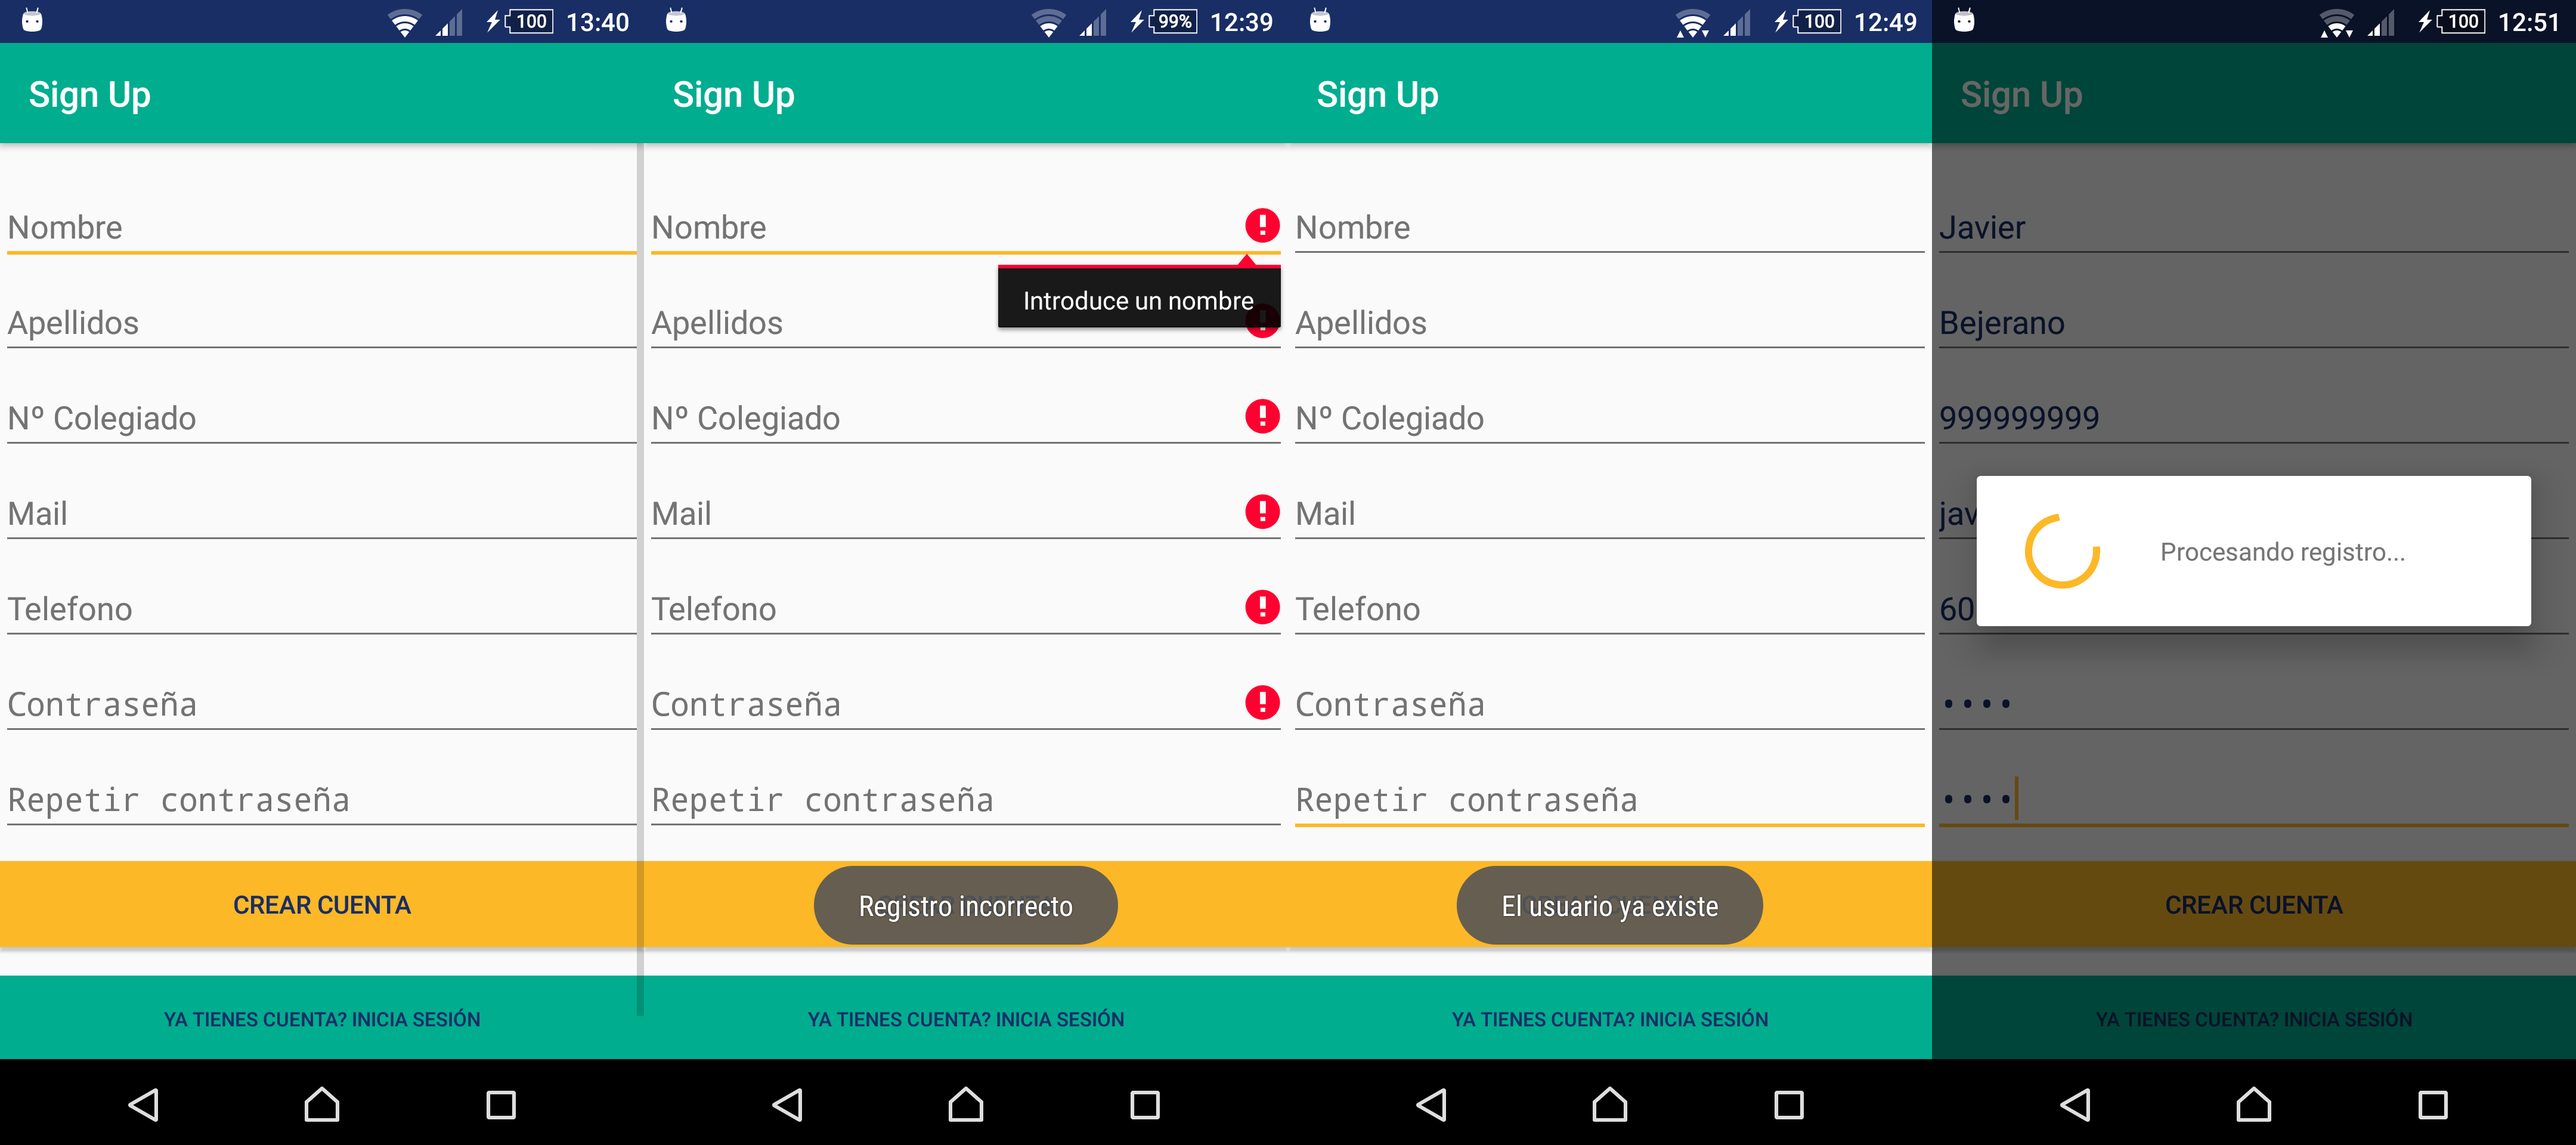
\includegraphics[height= 6.7cm]{capturas/sign_upFull.png}
\caption{Ventana - Registro}
\end{figure}

\begin{figure}[H]
\centering
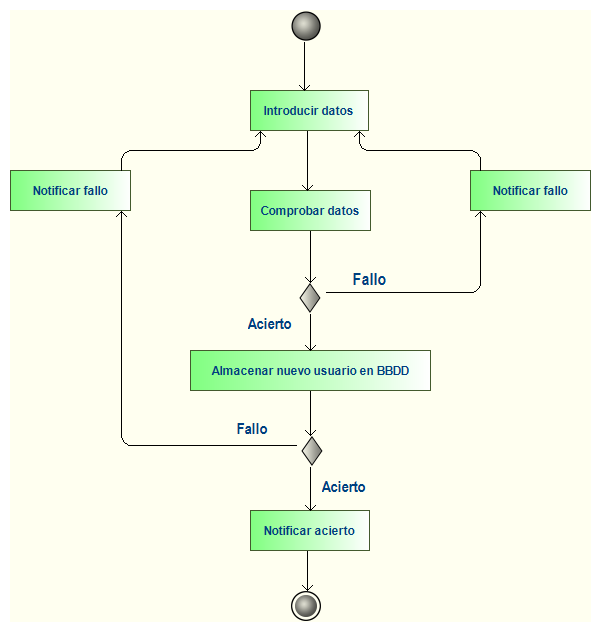
\includegraphics[height= 11cm]{diagramas/SignupActivitydiagram.png}
\caption{Diagrama de actividad - Registro}
\end{figure}

%MIS PACIENTES
\subsection {Mis pacientes}

Visualiza una lista con la información básica de tus pacientes, a saber, el ID, la edad y el género (M: Masculino, F: Femenino). Se ofrece la posibilidad de buscar haciendo uso del botón flotante de la parte inferior, así como compartir un paciente con otro médico manteniendo presionado su información asociada en la lista. Ambas posibilidades se describirán en profundidad posteriormente. 

\begin{figure}[H]
\centering
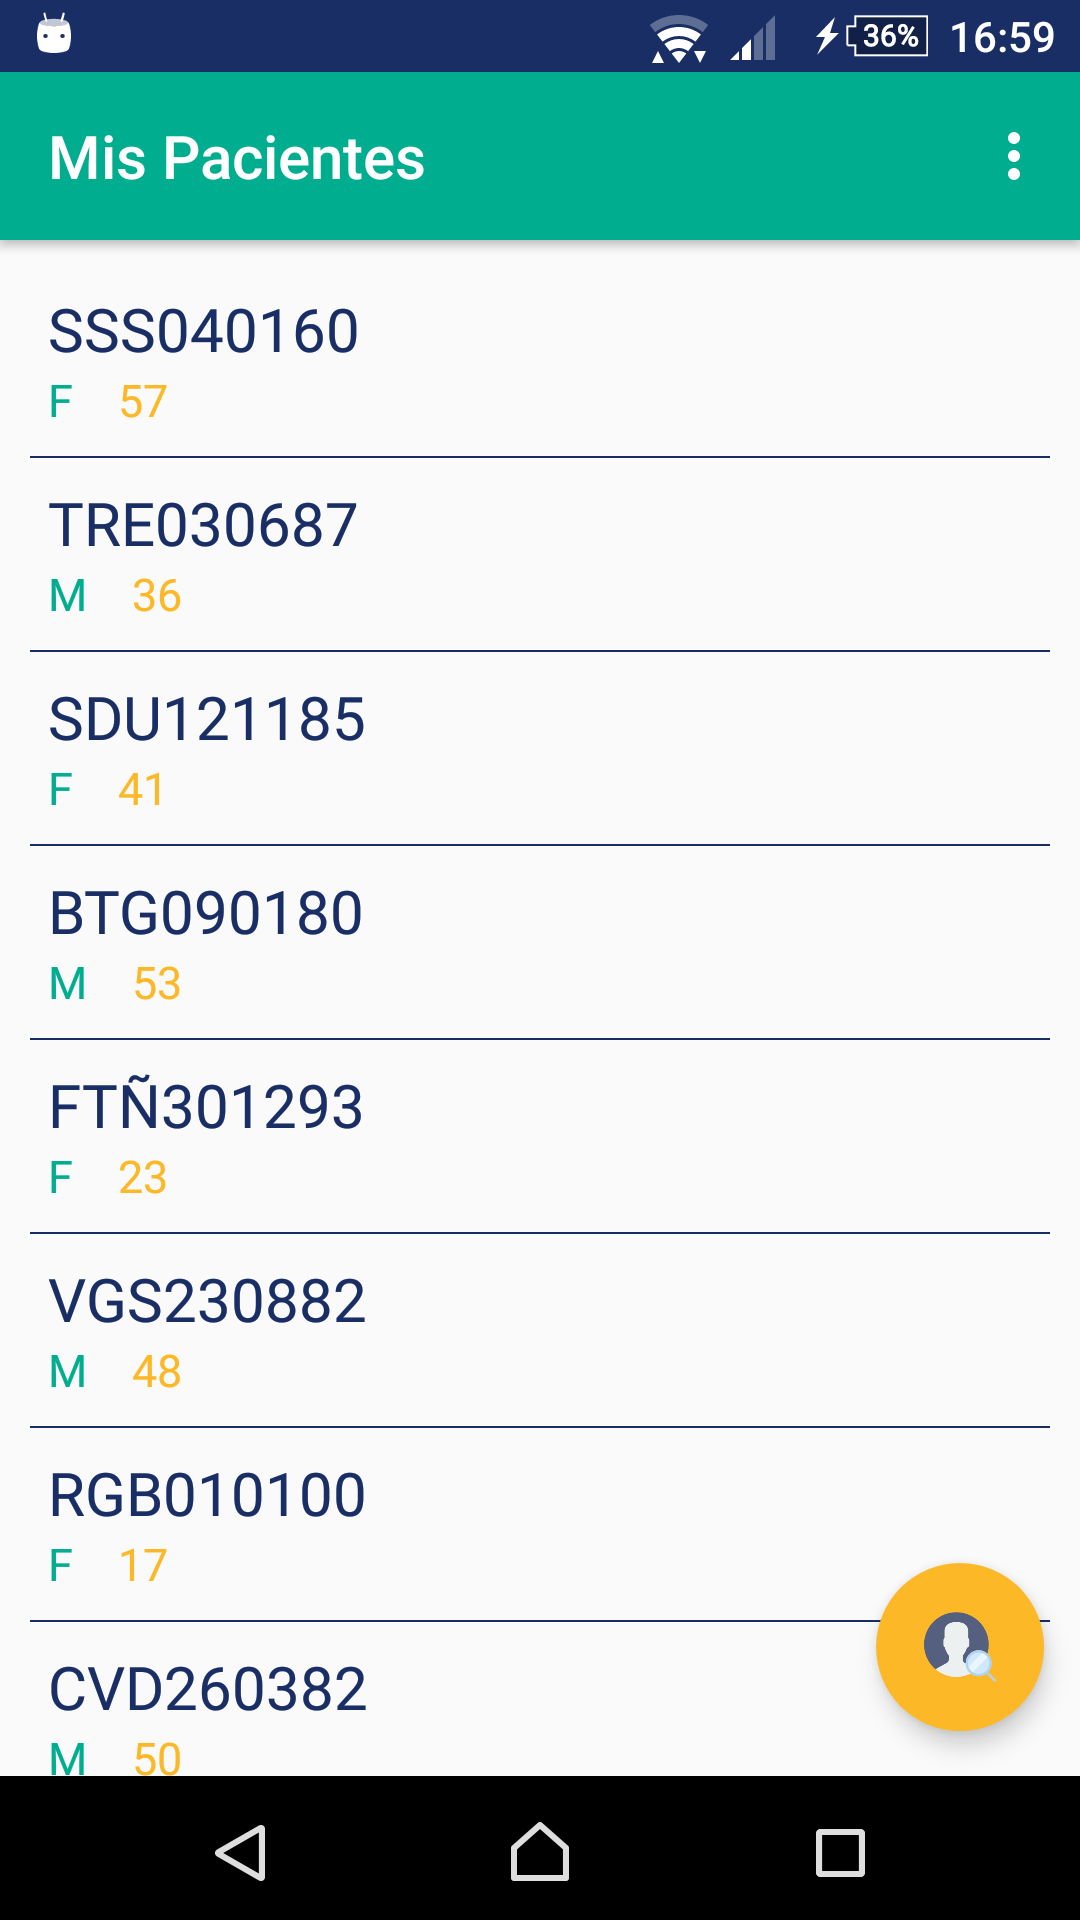
\includegraphics[height= 7cm]{capturas/mis_pacientes.png}
\caption{Ventana - Mis Pacientes}
\end{figure}

\begin{figure}[H]
\centering
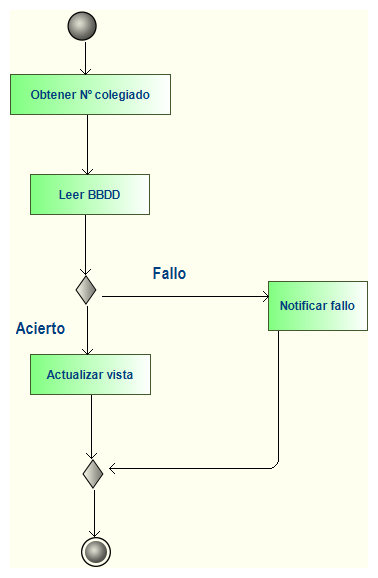
\includegraphics[height= 11cm]{diagramas/ListapacientesActivitydiagram.png}
\caption{Diagrama de actividad - Mis Pacientes}
\end{figure}

%COMPARTIR PACIENTE
\subsection {Compartir paciente}

La aplicación permite que un paciente sea tratado simultáneamente  por más de un médico. En esta ventana emergente el usuario introduce el número de colegiado del médico con el que quiere compartir los datos del paciente. Tras esta acción, este último quedará reflejado en la lista de pacientes del otro médico.

\begin{figure}[H]
\centering
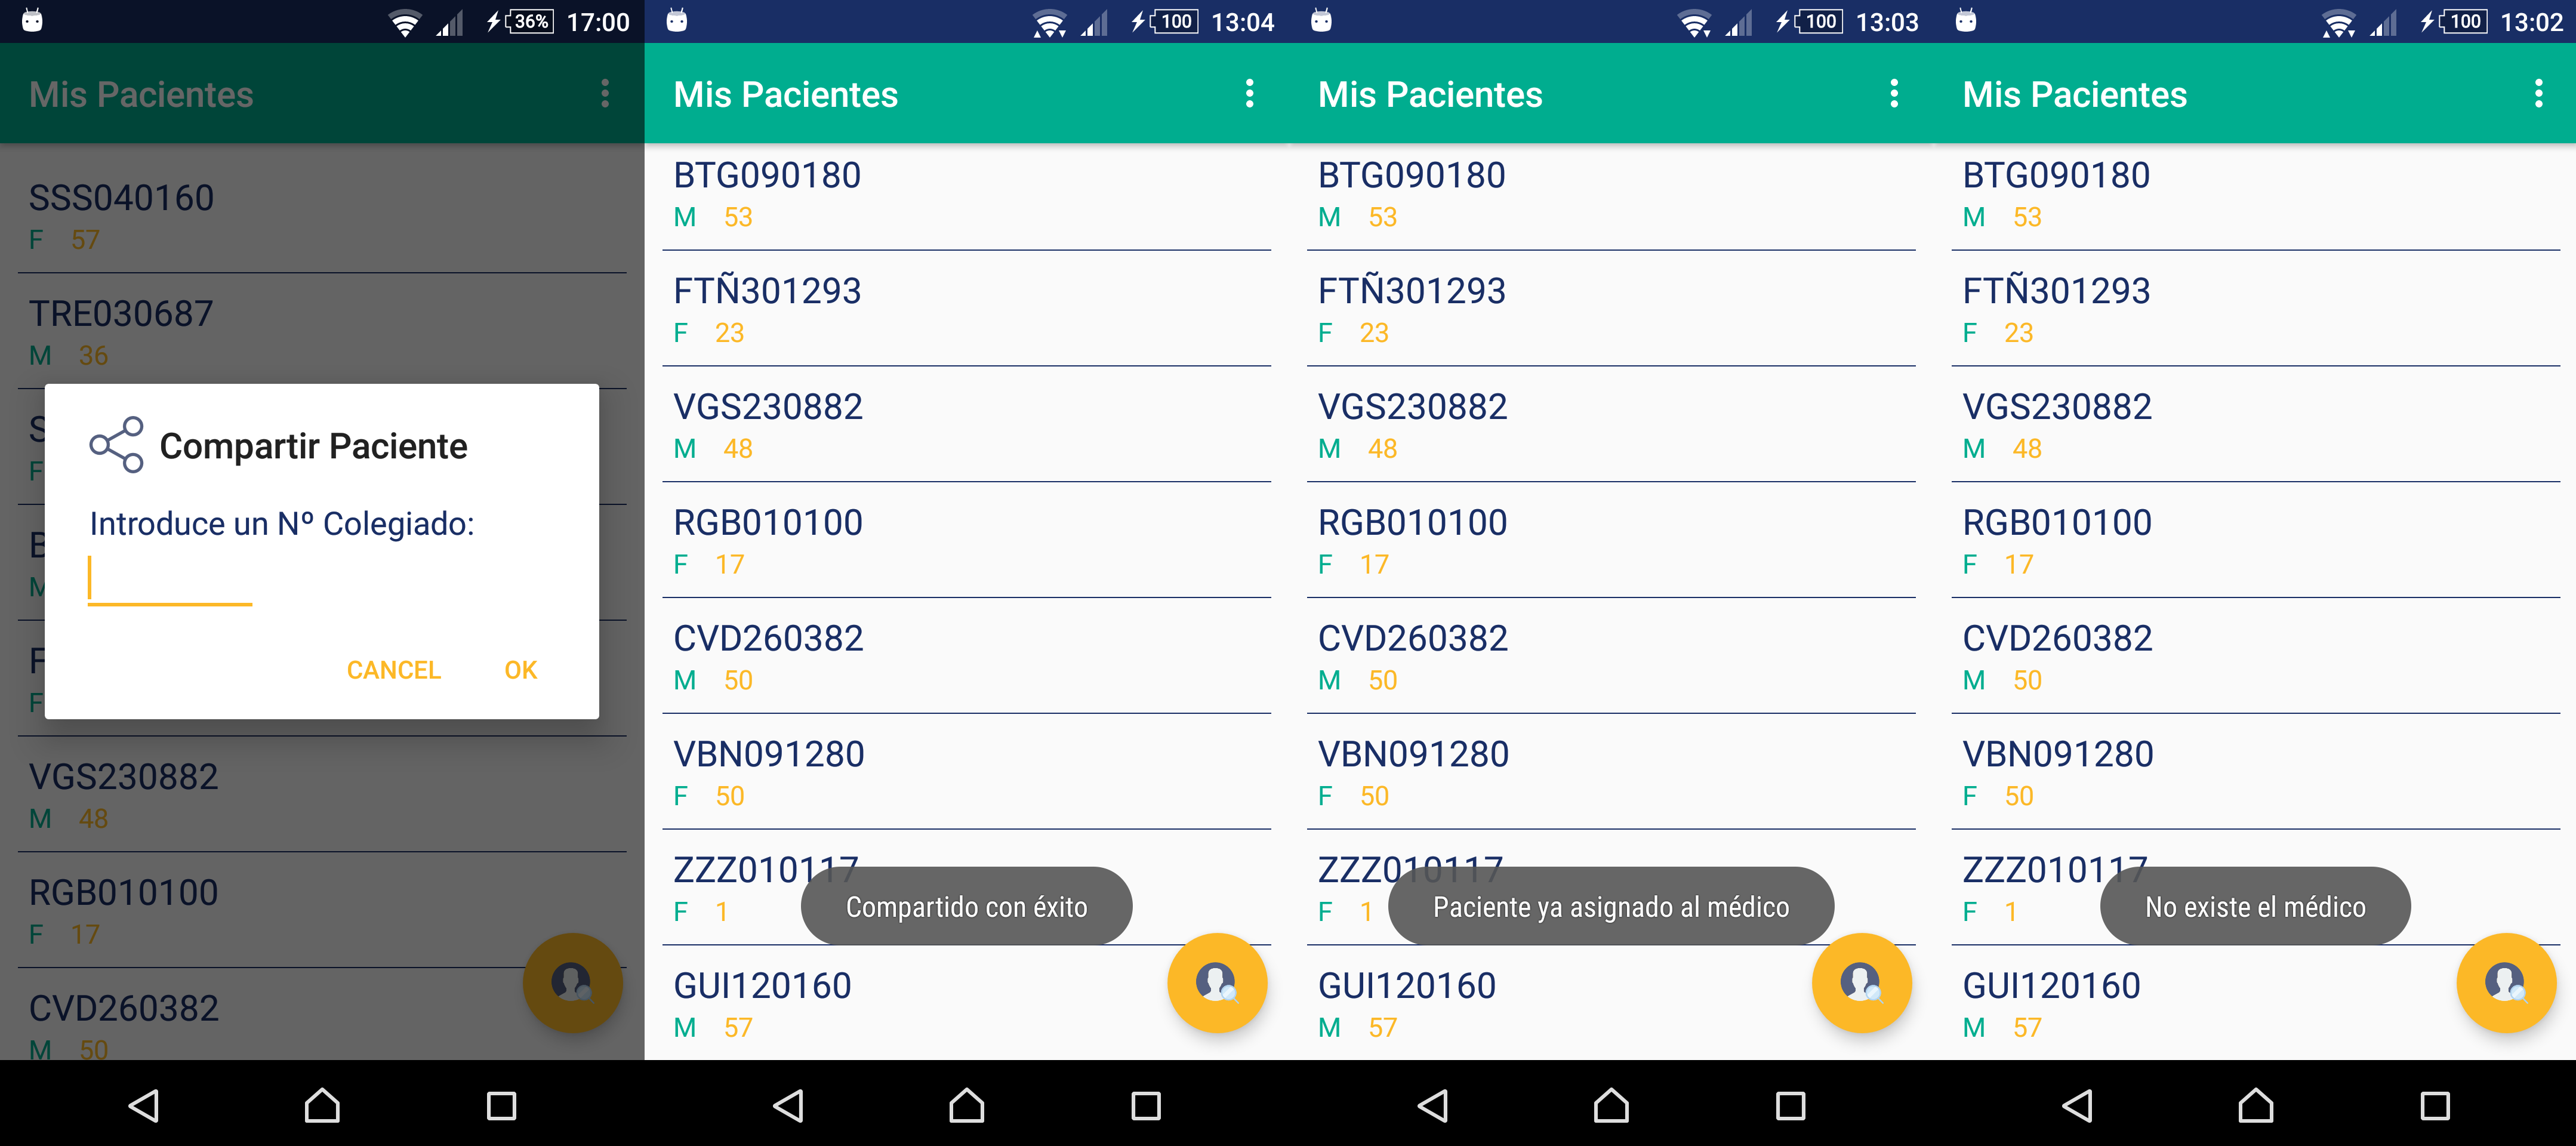
\includegraphics[height= 6.7cm]{capturas/compartir_pacienteFull.png}
\caption{Ventana - Compartir Paciente}
\end{figure}

\begin{figure}[H]
\centering
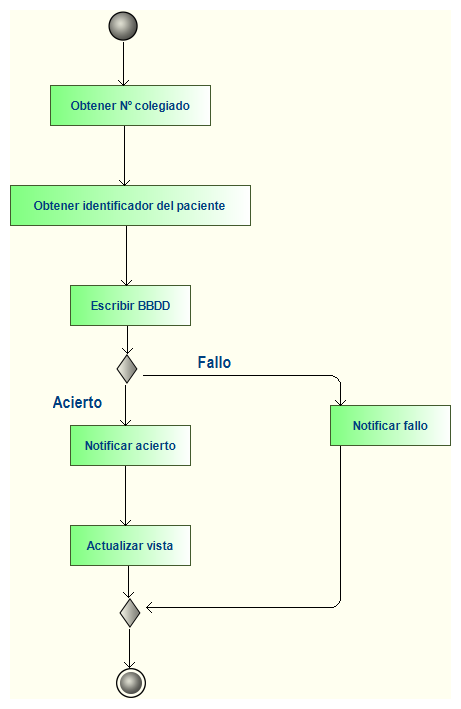
\includegraphics[height= 11cm]{diagramas/CompartirpacienteActivitydiagram.png}
\caption{Diagrama de actividad - Compartir Paciente}
\end{figure}

%BUSCAR PACIENTE
\subsection {Buscar paciente}

Para evitar los deméritos de una lista con una gran cantidad de pacientes se facilita una serie filtros que permita encontrar con mayor facilidad al paciente(s) deseado(s). Se puede realizar una búsqueda  por identificador (parcial o completo), sexo, edad o una combinación entre ellos. La aplicación informará sobre el resultado y los filtros utilizados. Un caso particular es el de la ausencia de filtros, el cual resultará en la obtención de todos los pacientes.

\begin{figure}[H]
\centering
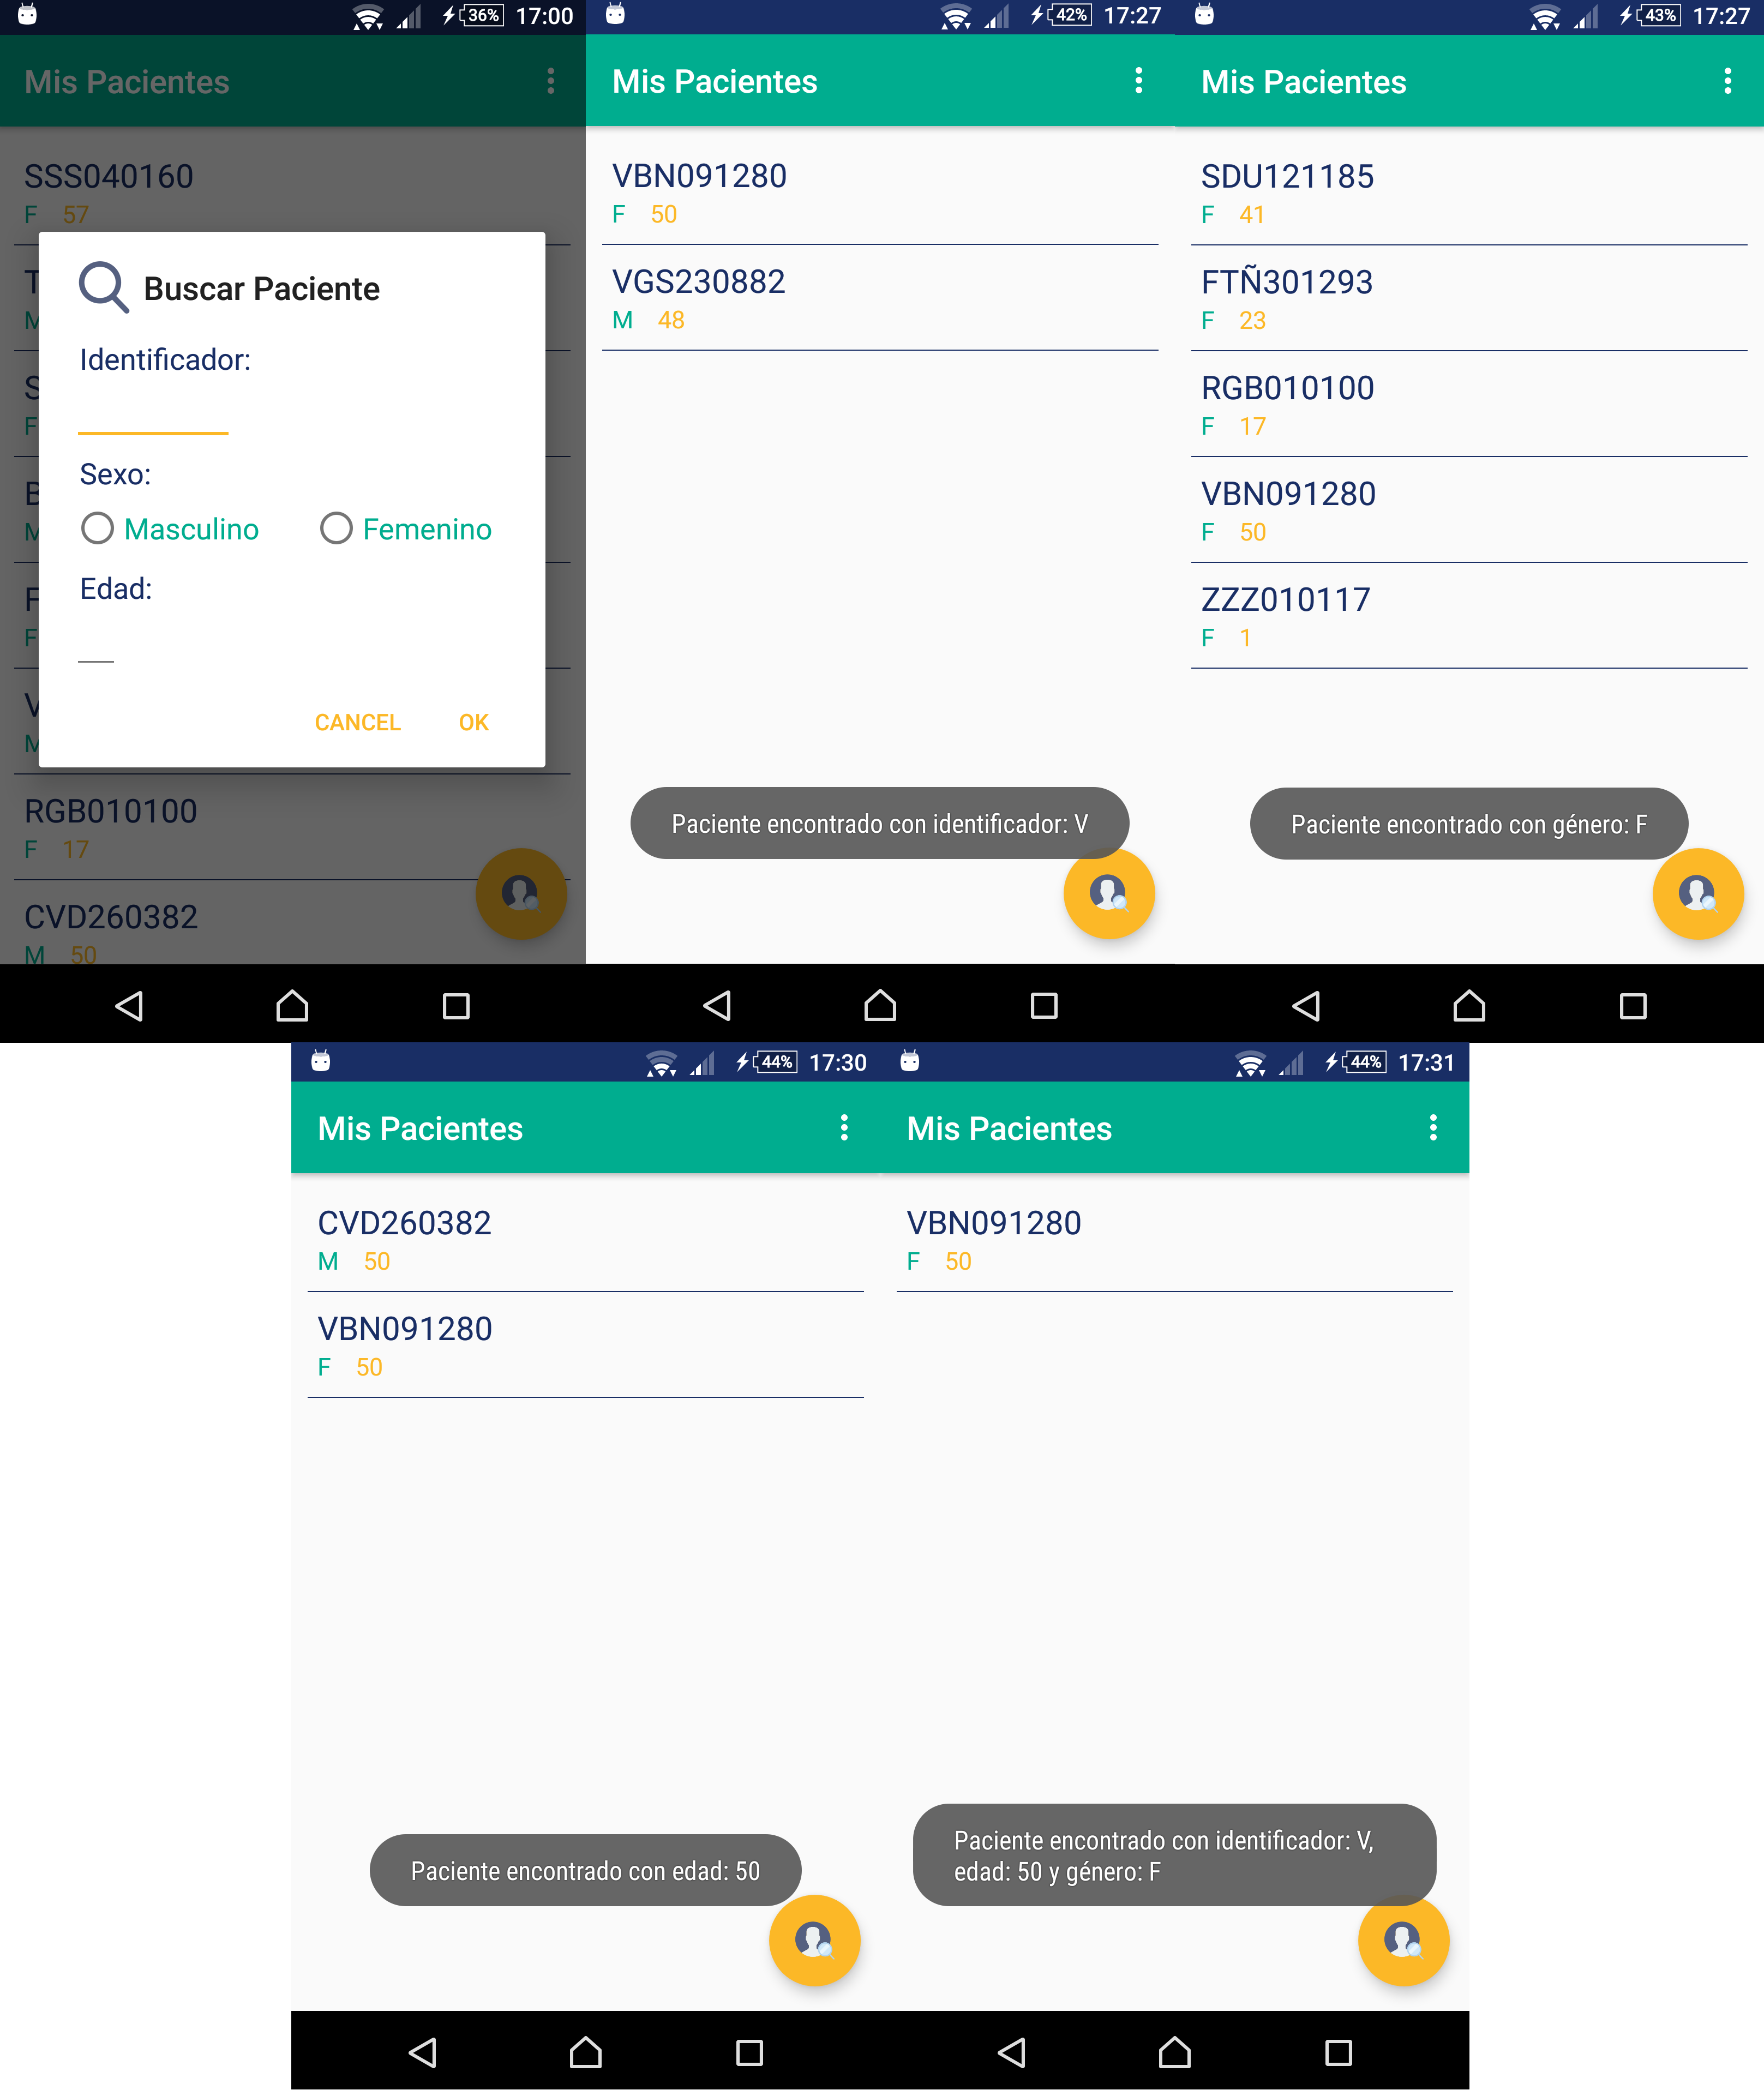
\includegraphics[height= 18cm]{capturas/buscarPacienteFull.png}
\caption{Ventana - Buscar Paciente}
\end{figure}

\begin{figure}[H]
\centering
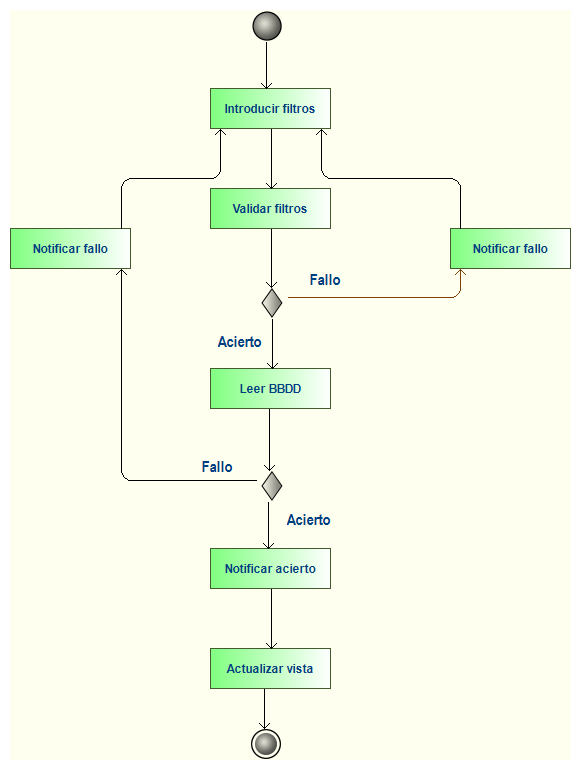
\includegraphics[height= 11cm]{diagramas/BuscarpacienteActivitydiagram.png}
\caption{Diagrama de actividad - Buscar Paciente}
\end{figure}

%CONSULTAR PACIENTE
\subsection {Consultar paciente}

En el caso de que se introduzcan datos erróneos en el alta del paciente o se desee actualizar la información del mismo, la app posibilita alterar dichos datos en esta ventana. También es posible remover al paciente de su lista personal. Además, sirve de punto de partida para las funcionalidades consistentes en calcular su riesgo cardiovascular, establecer el tratamiento y/o descargar el informe de su estado en formato PDF.

\begin{figure}[H]
\centering
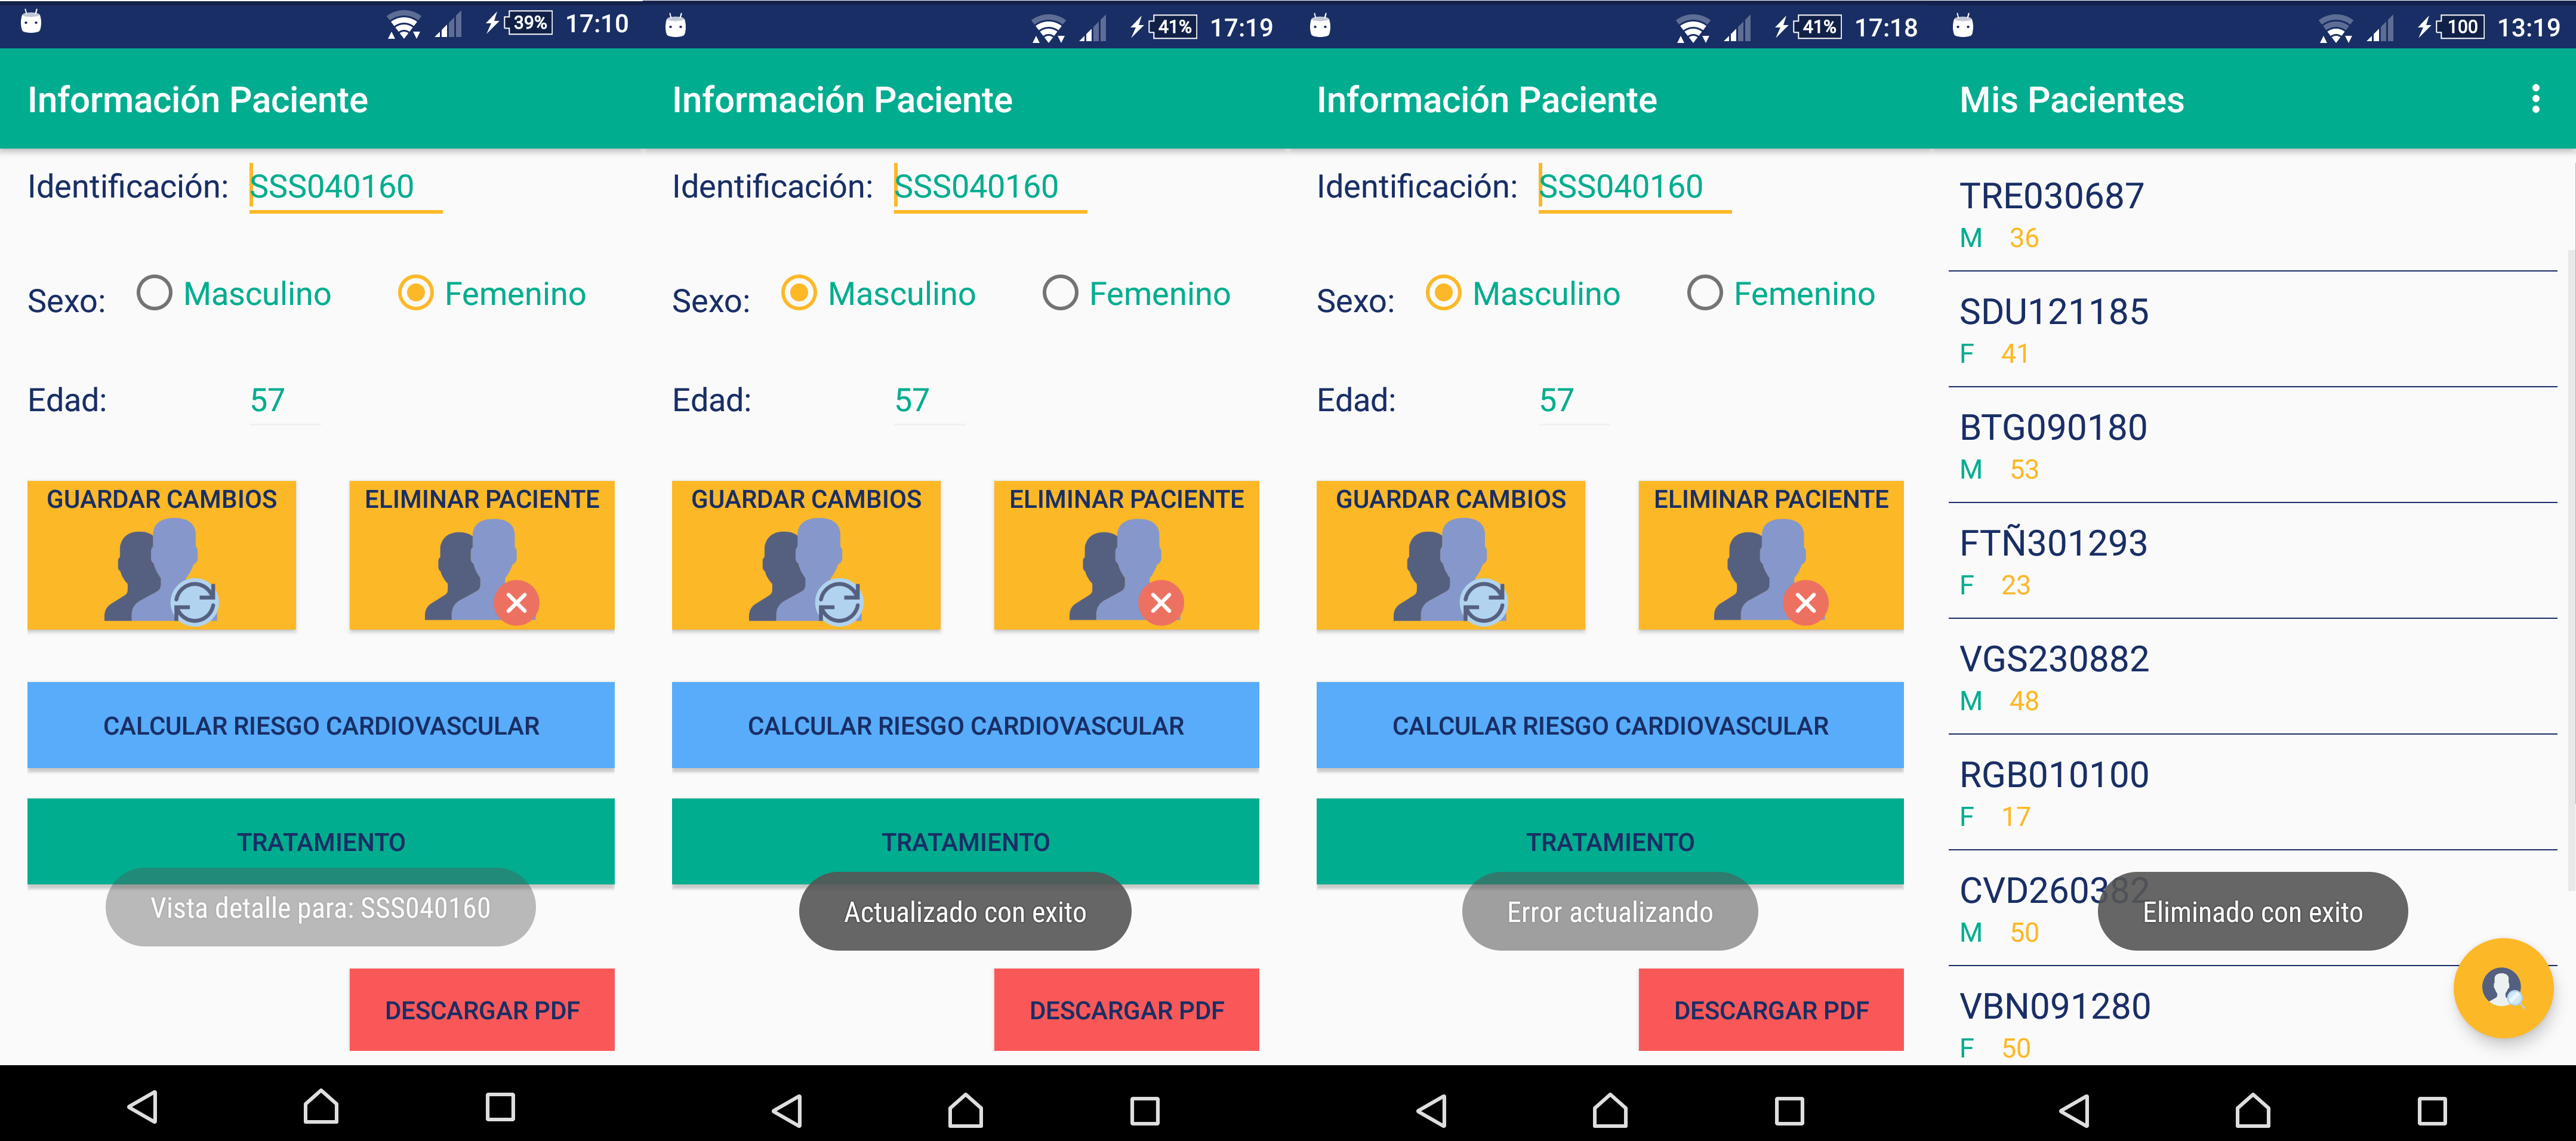
\includegraphics[height= 6.7cm]{capturas/infoPacienteFull2.png}
\caption{Ventana - Consultar Paciente}
\end{figure}

\begin{figure}[H]
\centering
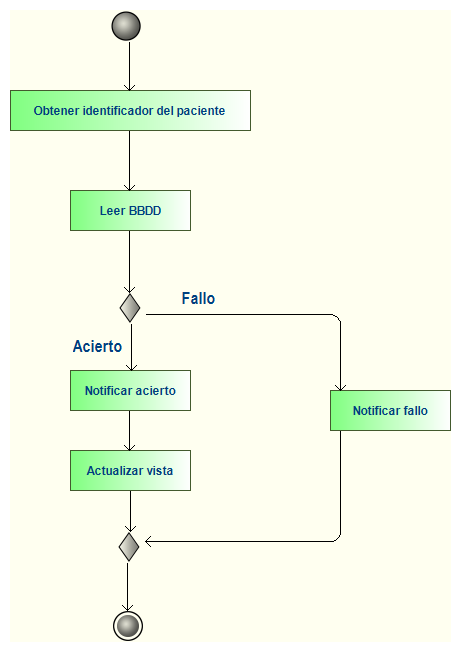
\includegraphics[height= 11cm]{diagramas/ConsultarpacienteActivitydiagram.png}
\caption{Diagrama de actividad - Consultar Paciente}
\end{figure}

\begin{figure}[H]
\centering
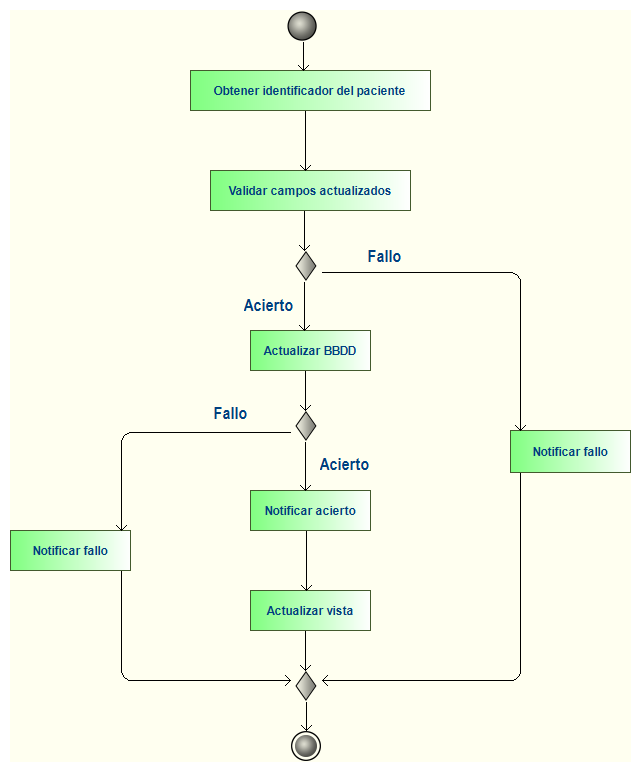
\includegraphics[height= 11cm]{diagramas/ActualizarpacienteActivitydiagram.png}
\caption{Diagrama de actividad - Actualizar Paciente}
\end{figure}

\begin{figure}[H]
\centering
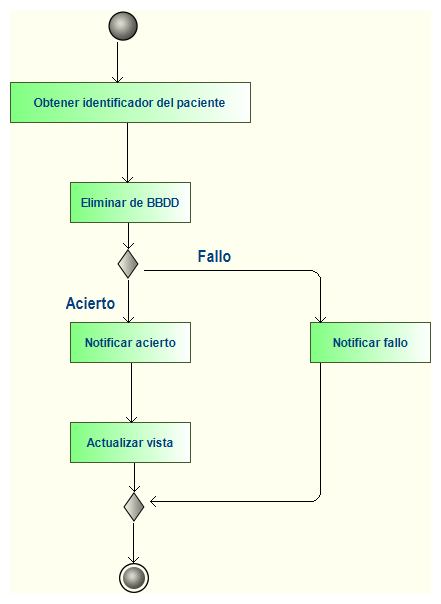
\includegraphics[height= 11cm]{diagramas/EliminarpacienteActivitydiagram.png}
\caption{Diagrama de actividad - Eliminar Paciente}
\end{figure}

%TABAQUISMO
\subsection {Calcular tabaquismo}

El hábito de fumar es uno de los aspectos más sobresalientes en el cálculo del riesgo cardiovascular. Nuestro fundamento es la fórmula  IPA (índice de paquete al año) que se define como número de cigarrillos al día multiplicado por los años de adicción, y dividido entre 20. La pantalla cuestiona por las dos entradas (cigarrillos y años) y devuelve el índice IPA calculado. De igual forma que en otros casos se anunciará el éxito o fracaso de la operación.

\begin{figure}[H]
\centering
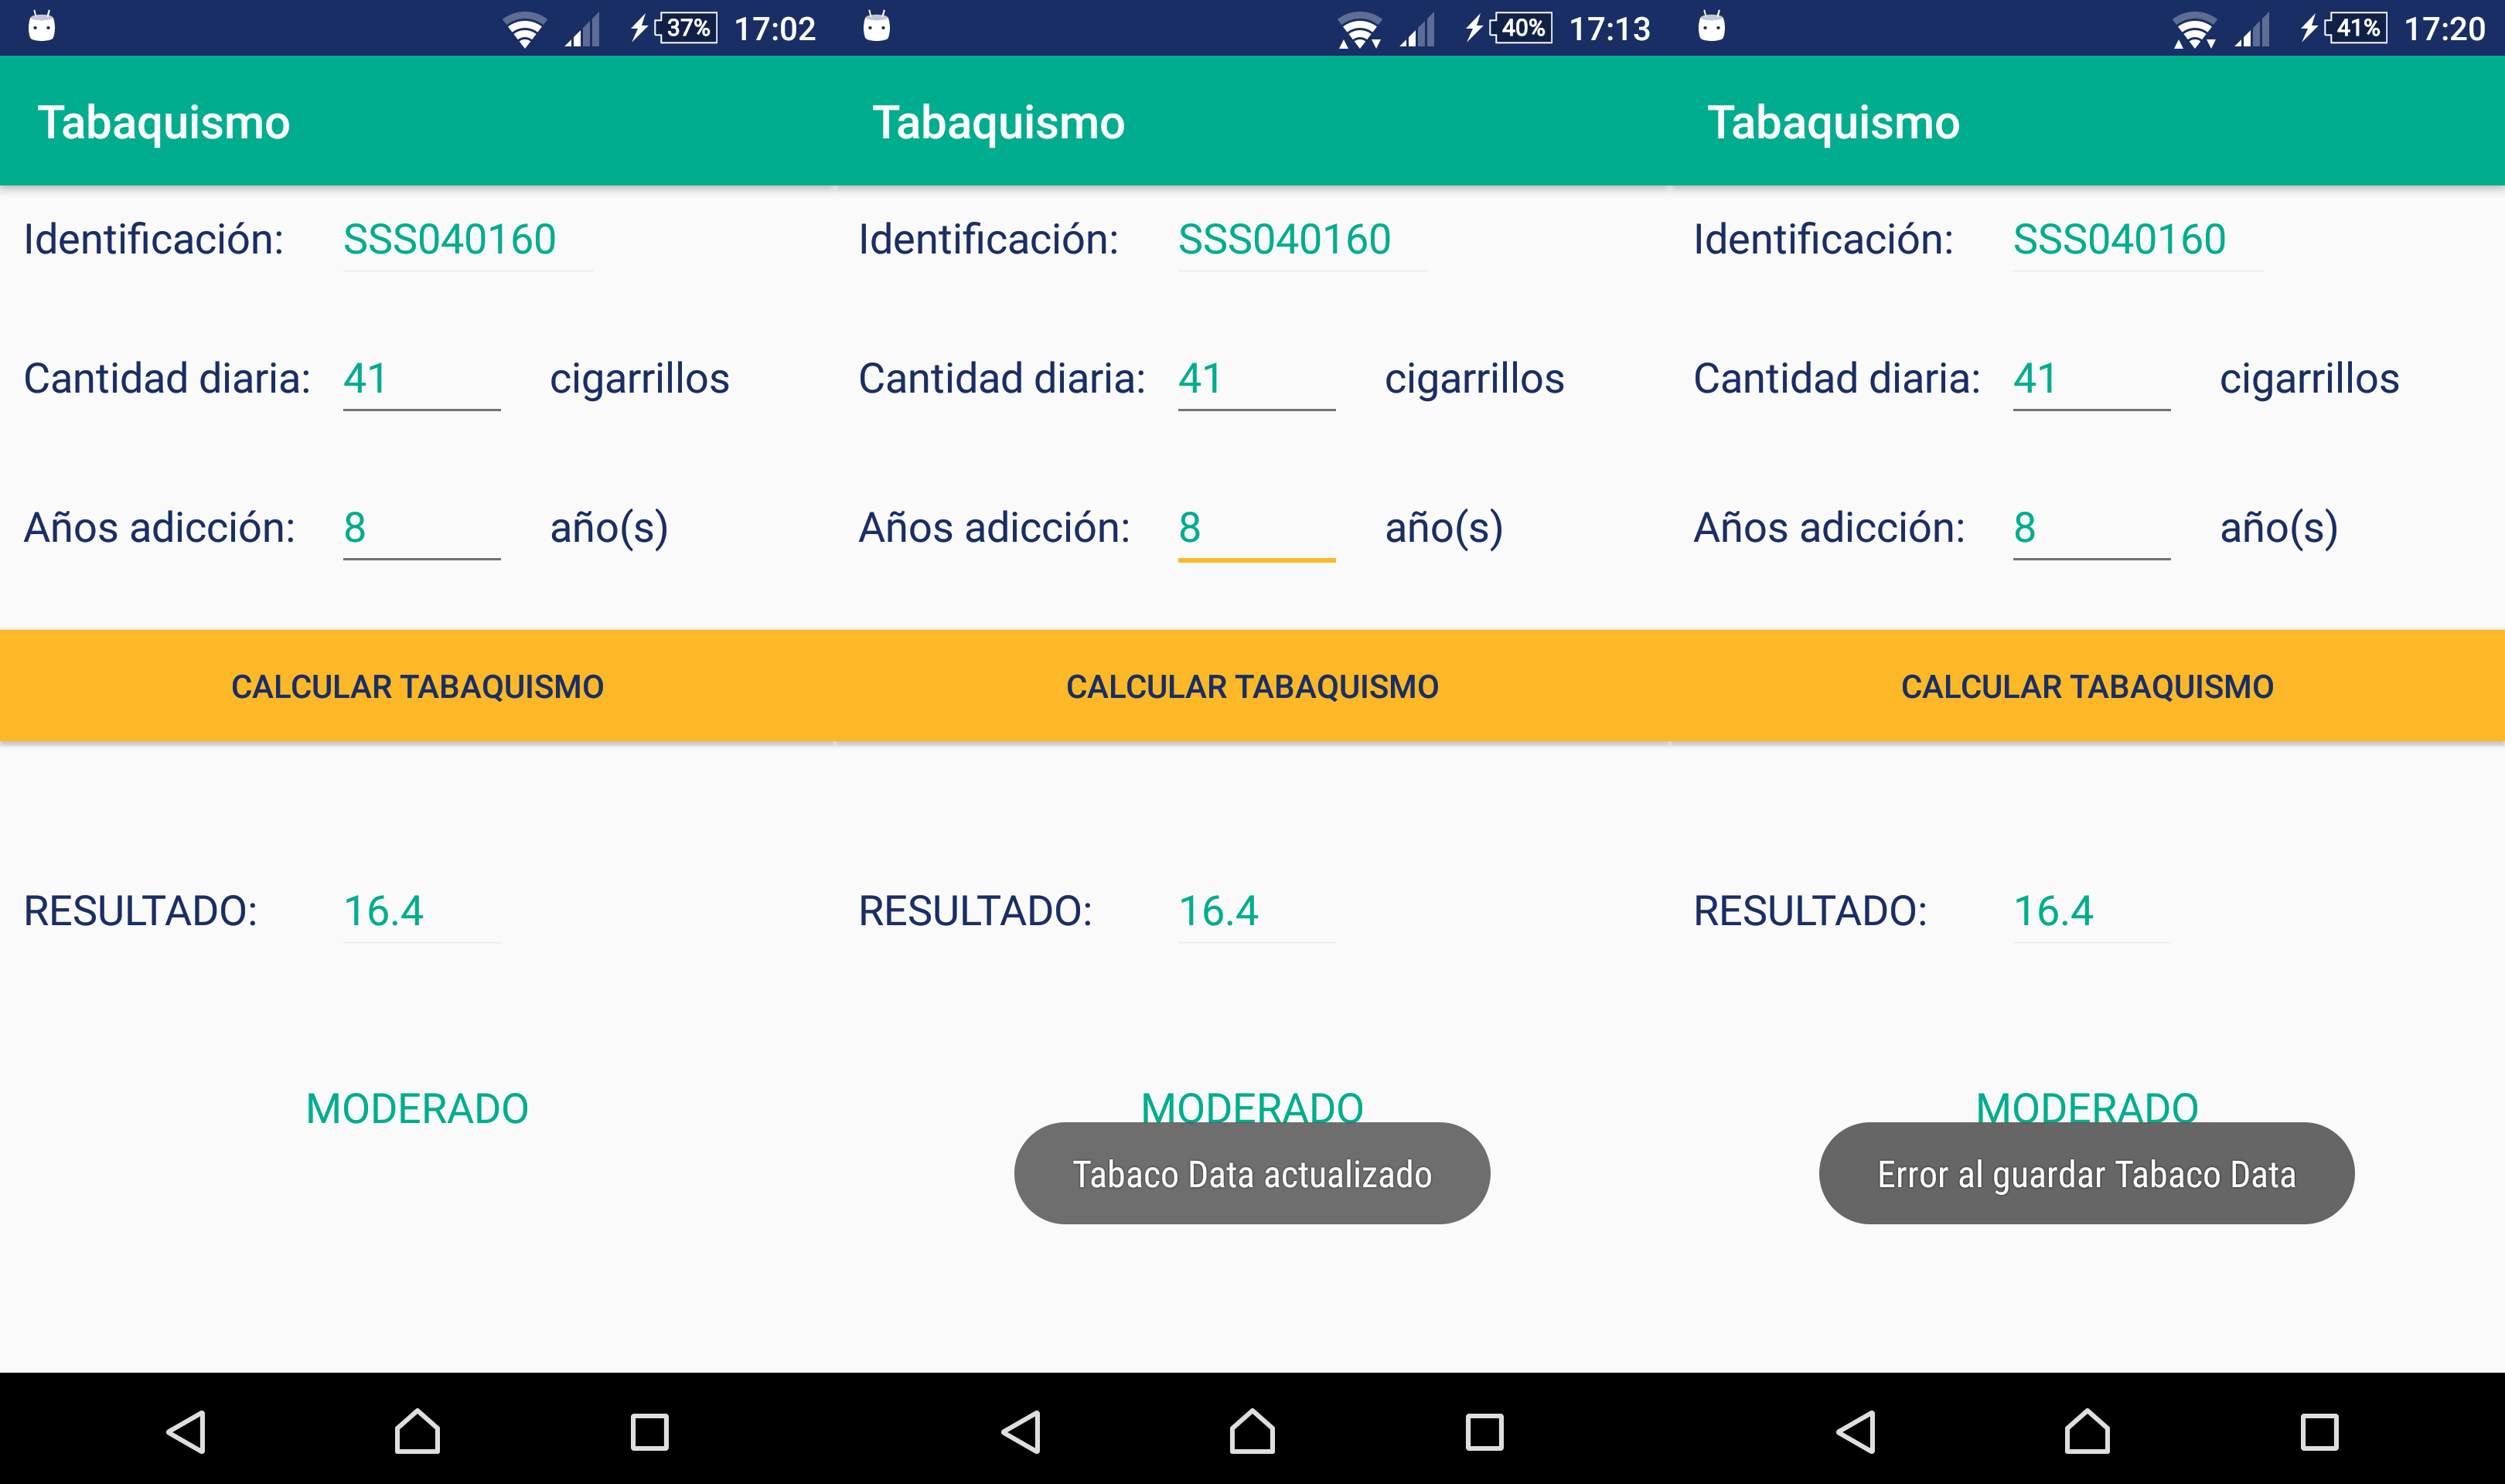
\includegraphics[height= 9cm]{capturas/tabaquismoFull.png}
\caption{Ventana - Tabaquismo}
\end{figure}

\begin{figure}[H]
\centering
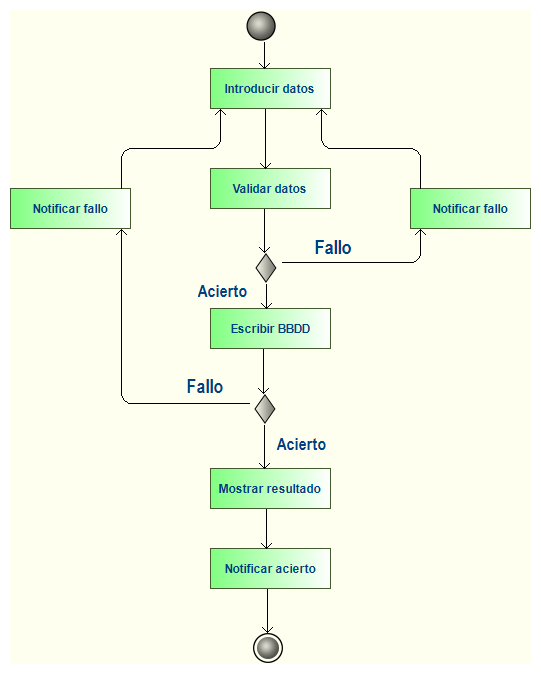
\includegraphics[height= 11cm]{diagramas/TabaquismoActivitydiagram.png}
\caption{Diagrama de actividad - Tabaquismo}
\end{figure}

%DIABETES
\subsection {Calcular diabetes}

La diabetes es el agente esencial entre los causantes de enfermedades cardiovasculares. Por esta razón nuestra app recauda numerosos campos de influencia para que el médico pueda determinar un tratamiento eficaz. Los datos solicitados: tipo de diabetes, tratamiento, hemoglobina glucosilada, monitor continuo de glucosa (CGM), años de enfermedad, fecha último fondo de ojos, creatinina, microalbuminuria, urea, afroamericano.

\begin{figure}[H]
\centering
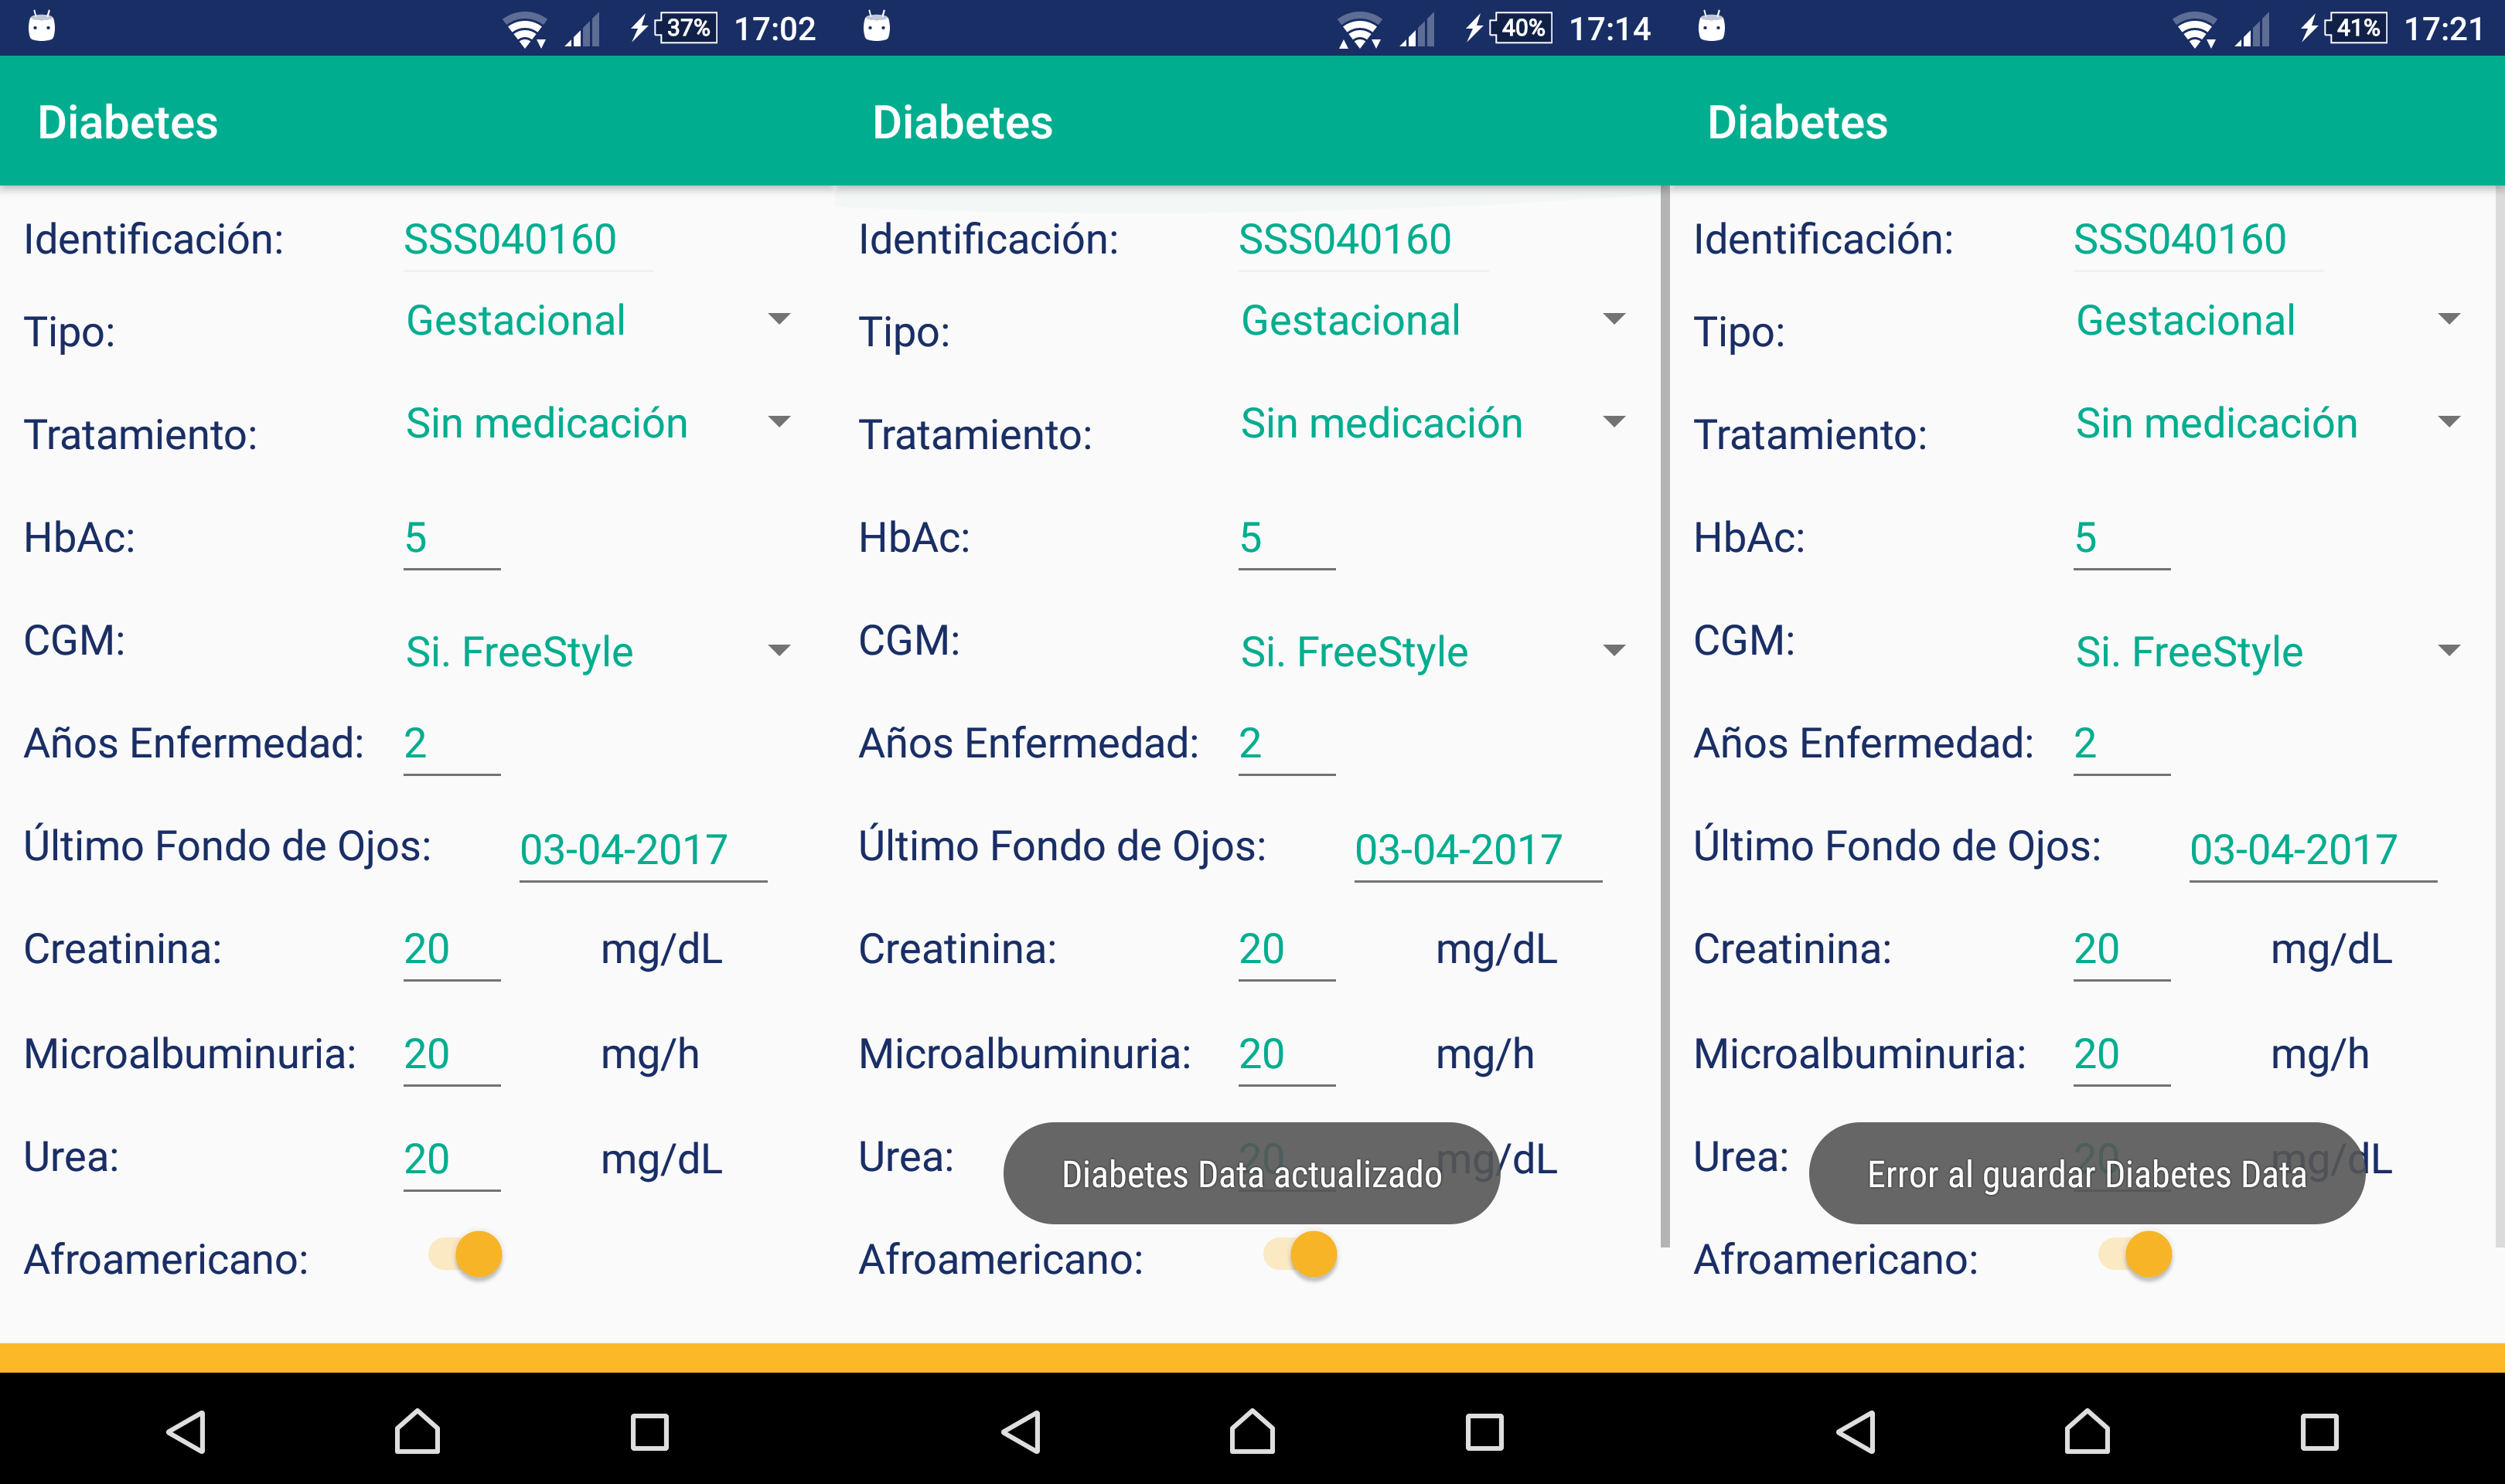
\includegraphics[height= 9cm]{capturas/diabetesFull.png}
\caption{Ventana - Diabetes}
\end{figure}

\begin{figure}[H]
\centering
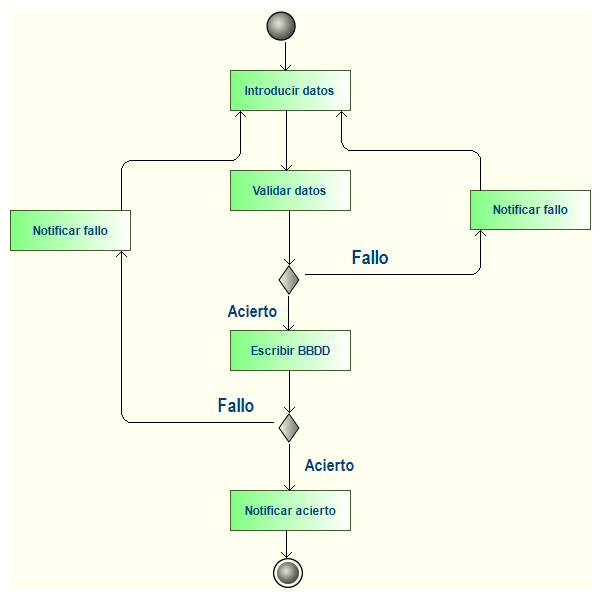
\includegraphics[height= 11cm]{diagramas/DiabetesActivitydiagram.png}
\caption{Diagrama de actividad - Diabetes}
\end{figure}

%COLESTEROL
\subsection {Calcular colesterol}

Deduce el valor de la lipoproteína de baja densidad (LDL) a partir de los valores asignados por el usuario a los parámetros de entrada, a saber, lipoproteína de alta densidad (HDL), colesterol total y la cantidad de triglicéridos del paciente.
Tanto los parámetros de entrada como los resultados obtenidos se definen en mg/dl. 

\begin{figure}[H]
\centering
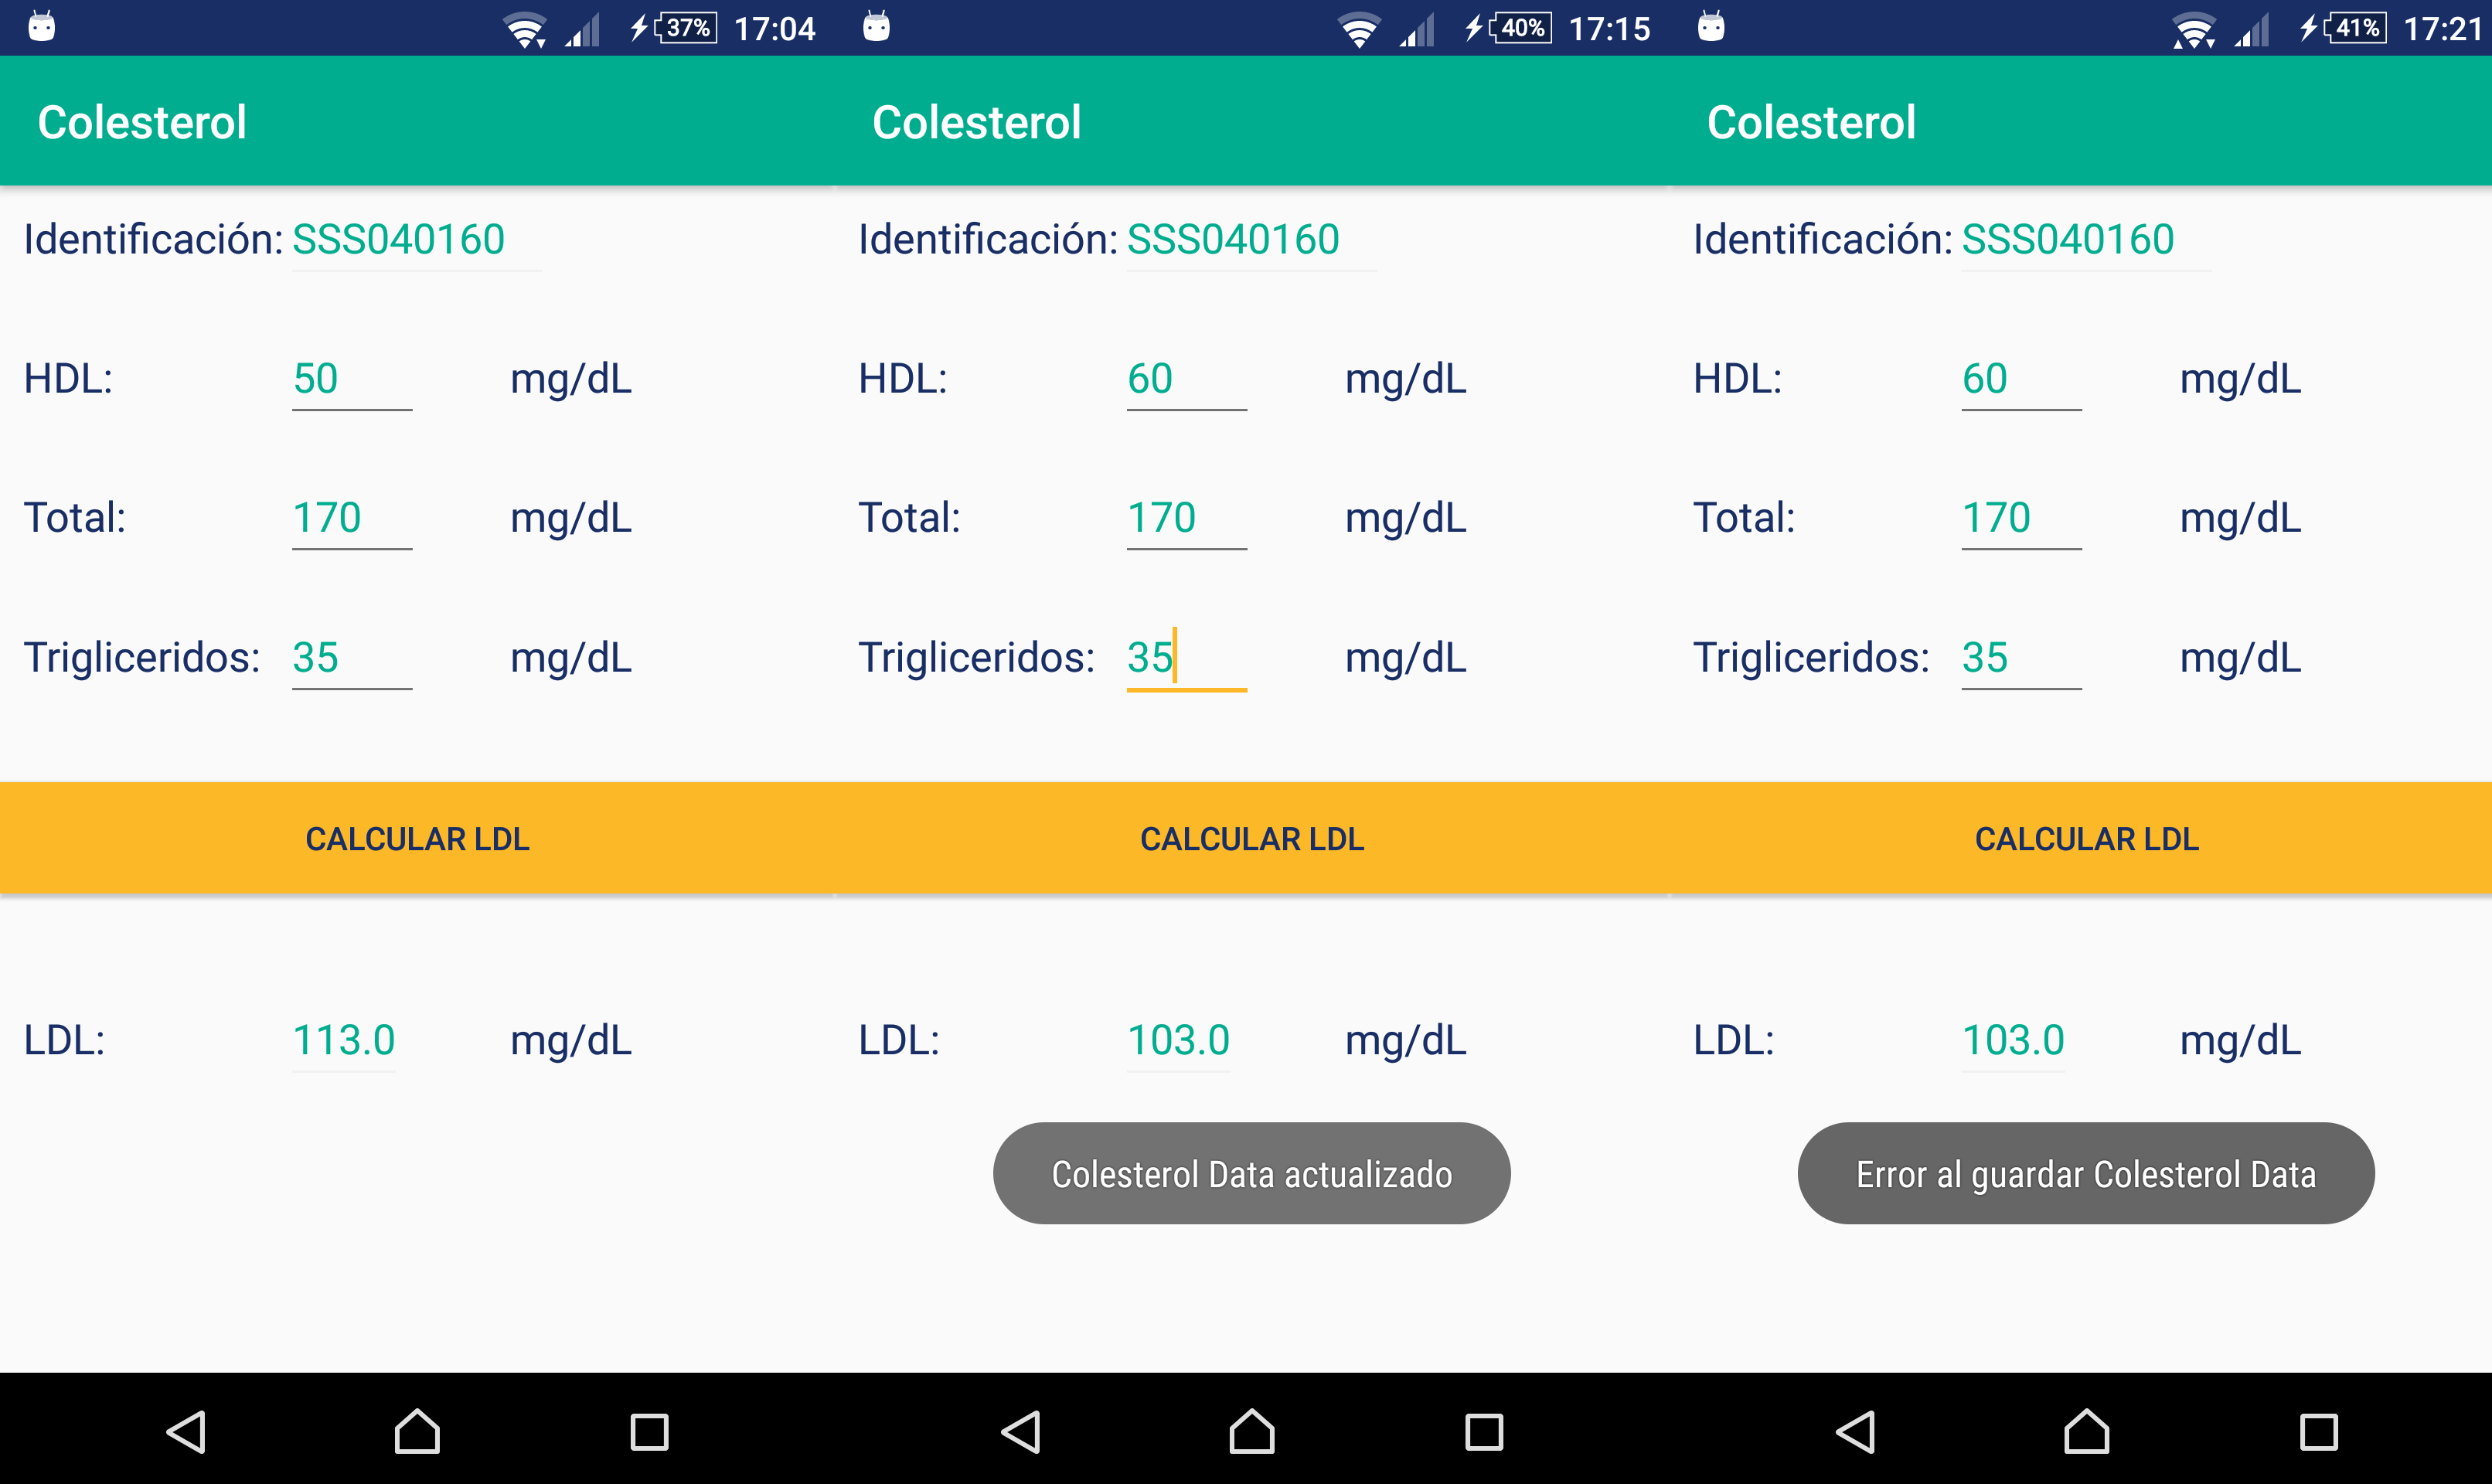
\includegraphics[height= 9cm]{capturas/colesterolFull.png}
\caption{Ventana - Colesterol}
\end{figure}

\begin{figure}[H]
\centering
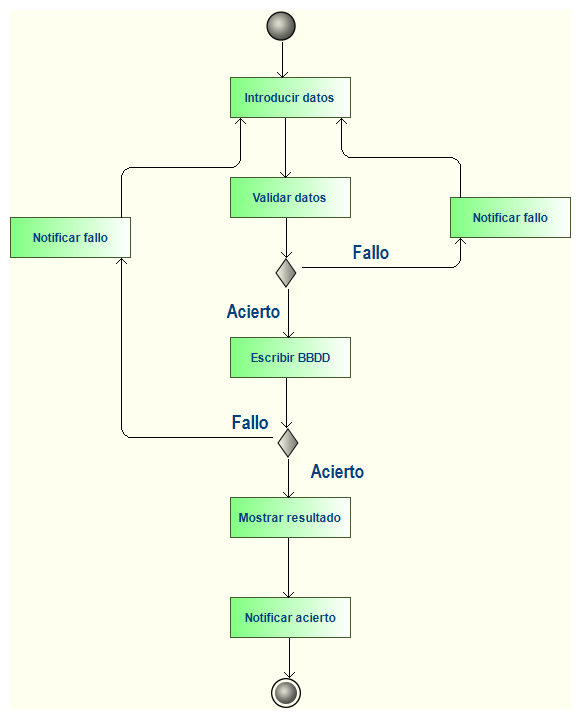
\includegraphics[height= 11cm]{diagramas/ColesterolpacienteActivitydiagram.png}
\caption{Diagrama de actividad - Colesterol}
\end{figure}

%HTA
\subsection {Calcular hipertensión arterial}

Este término se refiere a la hipertensión arterial, es decir, el fenómeno que sucede si el sujeto presenta una fuerza excesiva contra las paredes de las arterias a medida que el corazón bombea sangre a su cuerpo.
La aplicación solicita el valor que resulta del análisis de la presión arterial sistólica y diastólica. Los datos se expresan en mmHg.

Las conclusiones de la aplicación son comunicadas mediante un mensaje claro que varía en función de la información suministrada.
Es notable mencionar que, en principio, los rangos de diastólica suelen tener una estrecha relación con los intervalos de valores relativos a la presión arterial sistólica. Sin embargo, la presión arterial sistólica tiene una mayor influencia que la distólica en la determinación del HTA. En consecuencia, si se sucediese el caso en el que el valor de diastólica no entre en el conjunto de valores esperado la app decidirá el resultado en la forma habitual, pero mencionará dicha anomalía mediante un warning al médico.

\begin{figure}[H]
\centering
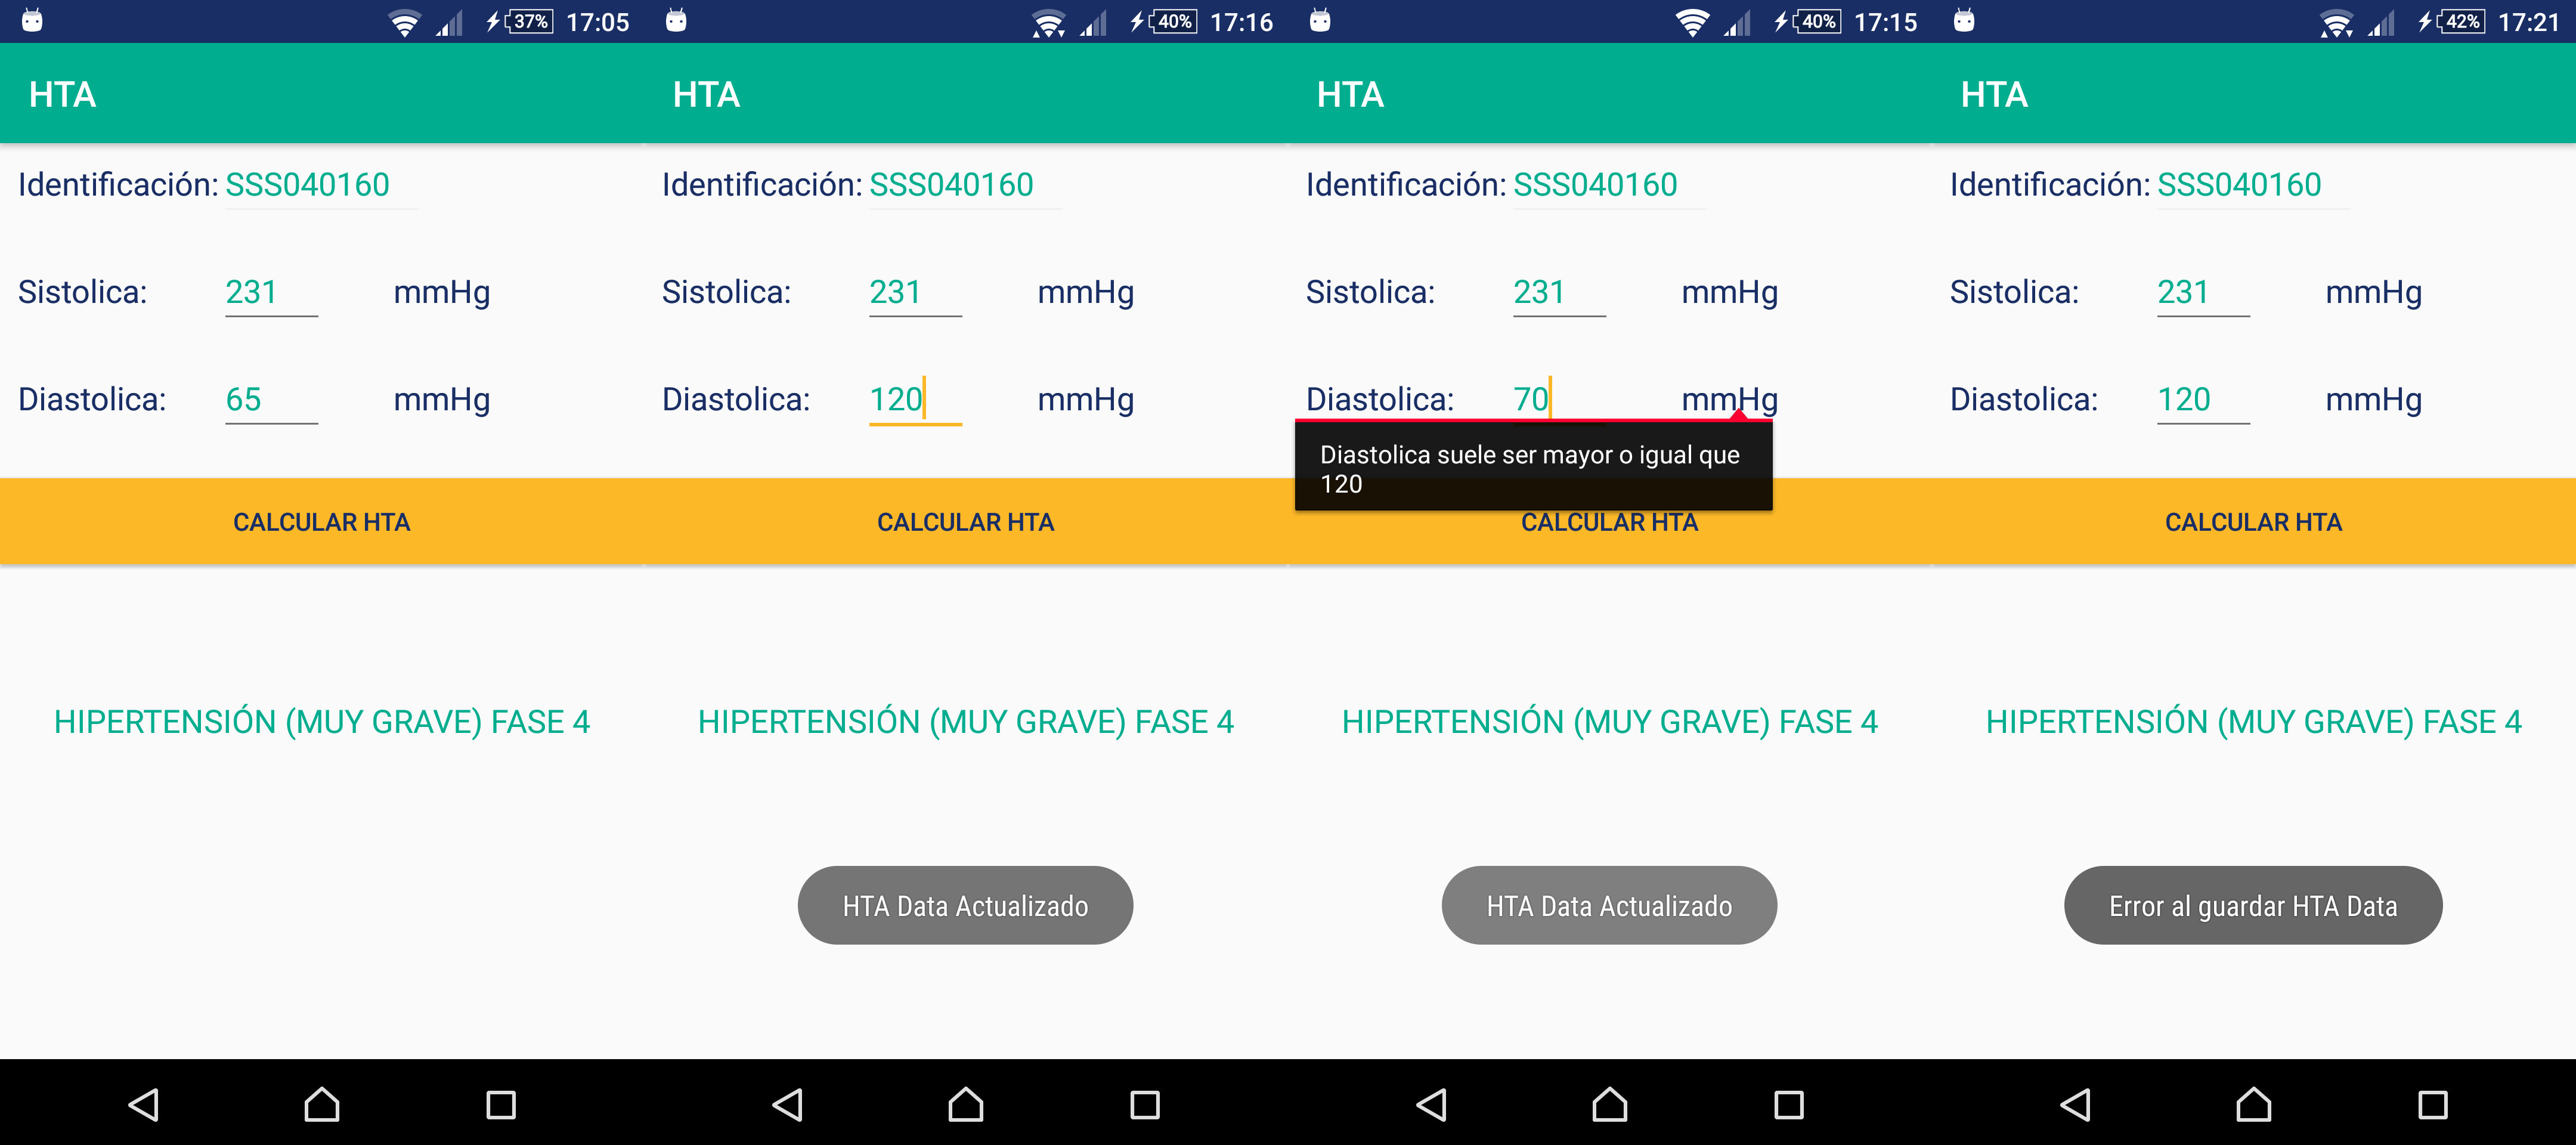
\includegraphics[height= 6.7cm]{capturas/HtaFull.png}
\caption{Ventana - Hipertensión Arterial}
\end{figure}

\begin{figure}[H]
\centering
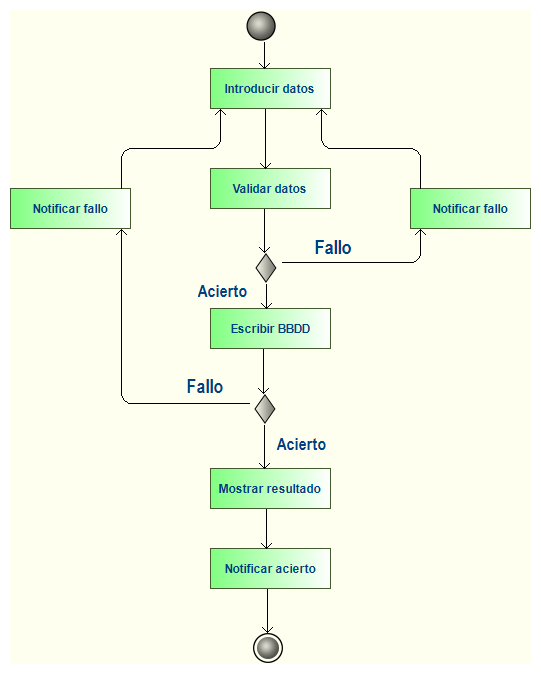
\includegraphics[height= 11cm]{diagramas/HtaActivitydiagram.png}
\caption{Diagrama de actividad - Hipertensión Arterial}
\end{figure}

%IMC
\subsection {Calcular índice de masa corporal}

De acuerdo con los estudios realizados, el IMC desempeña un rol significativo en los análisis del riesgo cardiovascular. Este índice establece una relación entre el peso y la altura y constituye un fiable indicativo para determinar casos de peso insuficiente, peso excesivo u obesidad en adultos. 
Atendiendo a la fórmula, los parámetros de entrada son el peso definido en kilogramos y la altura del individuo declarada en metros. El resultado se expresa en kg/m2. Asimismo, la aplicación interpreta el resultado obtenido y lo refleja en lenguaje cotidiano.

\begin{figure}[H]
\centering
\includegraphics[height= 9cm]{capturas/ImcFull.png}
\caption{Ventana - Índice de Masa Corporal}
\end{figure}

\begin{figure}[H]
\centering
\includegraphics[height= 11cm]{diagramas/ImcpacienteActivitydiagram.png}
\caption{Diagrama de actividad - Índice de Masa Corporal}
\end{figure}

%TRATAMIENTO
\subsection {Tratamiento}

En función de los datos recaudados sobre el paciente el médico tiene la posibilidad de dictar unas medidas para atender a las circunstancias del sujeto. Se dispone un resumen de la condición actual del paciente a partir de la cual el profesional pueda trabajar sin tener necesidad de consultar nuevamente los datos ofrecidos en otras pantallas.

\begin{figure}[H]
\centering
\includegraphics[height= 9cm]{capturas/TratamientoFull.png}
\caption{Ventana - Tratamiento}
\end{figure}

\begin{figure}[H]
\centering
\includegraphics[height= 11cm]{diagramas/TrataminetoActivitydiagram.png}
\caption{Diagrama de actividad - Tratamiento}
\end{figure}

%DESCARGAR PDF
\subsection {Descargar PDF}

Es de notable conveniencia disponer de un método para almacenar y transmitir la documentación obtenida en esta aplicación. La capacidad de exportar estos datos en formato PDF habilita un sistema sencillo para compartir esta información con el paciente, personales relacionadas con el mismo u otros individuos cualificados...  Esta táctica favorece las acciones en el evento de que quieras imprimirlo, y archivarlo o clasificarlo, fomentando así la portabilidad.

\begin{figure}[H]
\centering
\includegraphics[height= 9cm]{capturas/PDF_Full.png}
\caption{Ventana - Descargar PDF}
\end{figure}

\begin{figure}[H]
\centering
\includegraphics[height= 7cm]{diagramas/GenerarPDFActivitydiagram.png}
\caption{Diagrama de actividad - Descargar PDF}
\end{figure}

%CERRAR SESION
\subsection {Cerrar sesión}

Deja por concluida la actividad con su cuenta en la app. Esta última preguntará por confirmación de si realmente es su intención y no es una equivocación fortuita.

\begin{figure}[H]
\centering
\includegraphics[height= 7cm]{capturas/log_out.png}
\caption{Ventana - Cerrar Sesión}
\end{figure}

\begin{figure}[H]
\centering
\includegraphics[height= 11cm]{diagramas/LogoutActivitydiagram.png}
\caption{Diagrama de actividad -  Cerrar Sesión}
\end{figure}

%%%%%%%%%%%%%%%%%%%%%%%%%%%%%%%%%%%%%%%%%%%%%%%%%%%%%%%%%%%%%%%%%%%%%%%%%%%%%%%%%%%%%%%%%%%%%%%%%%%%%%%%%%%%%%%%%%%%%%%%%
%																	ARQUITECTURA DE LA APLICACIÓN     																		             %
%%%%%%%%%%%%%%%%%%%%%%%%%%%%%%%%%%%%%%%%%%%%%%%%%%%%%%%%%%%%%%%%%%%%%%%%%%%%%%%%%%%%%%%%%%%%%%%%%%%%%%%%%%%%%%%%%%%%%%%%%
\chapter{Arquitectura de la aplicaci\'on}

El sistema está formado de una aplicación Android para el uso de los médicos y de una base de datos relacional. Presentamos a continuación una descripción detallada de la arquitectura para cada módulo del proyecto. 

%ANDROID STUDIO
\section {Aplicación Android}

La aplicación es para dispositivos Android a partir de la versión X, que está actualmente es compatible con X de los teléfonos móviles de la población. Además tiene un nivel de API 21?.

Es la aplicación la principal y única fuente de datos, a través de la cual el médico puede tener en todo momento al alcance de su mano los datos de un paciente para consultar o actualizar la información del mismo. La aplicación móvil tiene como tarea principal poder obtener el índice de riesgo cardiovascular.

%BASE DE DATOS
\section {Base de datos}

La base de datos está alojada en una máquina virtual en un servidor, la cual su función es el almacenaje de la información generada por la aplicación.

Usamos bases de datos relacionales para guardar todos los datos, al tener una clave primaria que identifique a cada uno de manera única en su respectiva tabla. 

Descartamos el uso de bases de datos no relacionales, como MongoDB, ya que con los datos no solo se harían lecturas y escrituras, sino que además podrían ser modificados. Características más propias de una base de datos estructurada.

%SERVIDOR Y UNIDAD DE PROCESAMIENTO
\section {Servidor y unidad de porcesamiento}

%%%%%%%%%%%%%%%%%%%%%%%%%%%%%%%%%%%%%%%%%%%%%%%%%%%%%%%%%%%%%%%%%%%%%%%%%%%%%%%%%%%%%%%%%%%%%%%%%%%%%%%%%%%%%%%%%%%%%%%%%
%																		MODELO DE DATOS    																		                       %
%%%%%%%%%%%%%%%%%%%%%%%%%%%%%%%%%%%%%%%%%%%%%%%%%%%%%%%%%%%%%%%%%%%%%%%%%%%%%%%%%%%%%%%%%%%%%%%%%%%%%%%%%%%%%%%%%%%%%%%%%
\chapter{Modelo de datos}

En nuestro es de vital importancia el tratamiento de una gran cantidad de datos, ya que estos son lo base para llevar acabo los fines de nuestra aplicación. En un estudio inicial concluimos que en nuestra aplicación se distinguían dos grupos principales, usuarios y médicos. 

Se utilizó MySQL para abordar este problema, puesto que es perfecta tanto para el desecho de información como para las búsquedas específicas y actualizaciones de datos.

Describimos en detalle las principales características del modelo de datos.

Nuestro enfoque es apoyarnos en el diagrama entidad-relación en conjunción con el relacional para su diseño. Tras terminar el proceso anterior, usamos la herramienta MySQL Workbench para obtener un diagrama que permita presentar los contenidos con un perfil visual atractivo.

\noindent
\begin{figure}[H]
\centering
\includegraphics[height= 11cm]{bd_model.png}
\caption{Base de datos relacional}
\end{figure}

Contamos con 10 tablas relacionadas entre sí mediante claves foráneas y atributos por medio de una estructura clara y eficiente.

\noindent
\textbf {medico\_validar}

Engloba la información relativa a los aspirantes a médico en nuestra aplicación. Estos datos son los que permitirán al administrador decidir si validar a la persona asociada como profesional sanitario.
\begin{itemize}
	\item id: clave primaria autoincremental.
	\item nombre: guarda el nombre del aspirante.
	\item apellidos: guarda los apellidos del solicitante.
	\item telefono: contiene el teléfono del aspirante.
	\item password: almacena la contraseña del aspirante.
	\item colegiado: guarda el número del colegiado (9 dígitos) del solicitante.
	\item mail: contiene el correo del candidato.
\end{itemize}

\noindent
\textbf {medico}

Especifica los datos personales del médico.
\begin{itemize}	
	\item nombre: contiene el nombre del médico.
	\item apellidos: guarda los apellidos del médico.
	\item telefono: almacena el teléfono del médico.
	\item password: contiene la contraseña del médico.
	\item colegiado: almacena el número del colegiado (9 dígitos) del médico. Es la clave primária porque debe definir unívocamente al profesional.
	\item mail: guarda el correo del médico.
\end{itemize}

\noindent
\textbf {medico\_roles}

Diferencia entre los distintos niveles de permisos concedidos a cada usuario.
\begin{itemize}
	\item id: clave primaria autoincremental.
	\item colegiado: referencia al identificador único del médico.
	\item rol: define si el profesional tiene privilegios administrativos (0) o no (1).
\end{itemize}

\noindent
\textbf {medico\_paciente}

Relaciona cada paciente con su(s) médico(s) asociado(s).
\begin{itemize}
	\item id: clave primaria autoincremental.
	\item colegiado: referencia al identificador único del médico.
	\item paciente\_id: referencia al identificador único del paciente.
\end{itemize}

\noindent
\textbf {pacientes}

Especifica los datos más importantes de cada paciente.
\begin{itemize}
	\item paciente\_id: clave primaria que define al paciente. Consiste en las tres iniciales de nombre y apellidos seguido de la fecha de nacimiento formato ddmmyy.
	\item sexo: establece el género del paciente. M (Masculino), F (Femenino).
	\item edad: guarda la edad del paciente.
	\item regicor: índice de riesgo cardiovascular expresado en tanto por ciento.
	\item finalTratamiento: almacena la información relativa al tratamiento específico designado por el médico para las circunstancias del paciente.
\end{itemize}

\noindent
\textbf {tabaquismo}

Relaciona cada paciente con su registro de tabaquismo.
\begin{itemize}
	\item pacienteId: referencia al identificador único del paciente.
	\item cantidad: cigarrillos consumidos por el paciente en un día.
	\item adiccion: designa los años de vicio del paciente.
	\item ipa: archiva el índice de paquetes al año.
\end{itemize}

\noindent
\textbf {imc}

Vincula cada paciente con la información relativa al imc.
\begin{itemize}
	\item pacienteId: referencia al identificador único del paciente.
	\item altura: contiene la estatura en metros del paciente.
	\item peso: almacena el peso en kilogramos del paciente.
	\item imc: guarda el ínidce de masa corporal.
\end{itemize}

\noindent
\textbf {hta}

Establece una conexión entre el paciente y los datos de hipertensión arterial.
\begin{itemize}
	\item pacienteId: referencia al identificador único del paciente.
	\item sistolica: almacena la presión arterial sistólica del paciente (mmHg).
	\item distolica: contiene la presión arterial diastólica del paciente (mmHg).
\end{itemize}

\noindent
\textbf {colesterol}

Relaciona cada paciente con sus valores de colesterol.
\begin{itemize}
	\item pacienteId: referencia al identificador único del paciente. 
	\item total: almacena la cantidad de colesterol total del paciente (mg/dl).
	\item hdl: contiene la cantidad de colesterol bueno del paciente (mm/dl).
	\item trigliceridos: almacena el nivel de trigliceridos en sangre del paciente (mm/dl).
	\item ldl: guarda la cantidad de colesterol malo del paciente (mm/dl).
\end{itemize}

\noindent
\textbf {diabetes}

Enlaza cada paciente con la información concerniente a su estado de diabetes.
\begin{itemize}
	\item pacienteId: referencia al identificador único del paciente. 
	\item tipo: designa el tipo de diabetes del paciente.
	\item tratamiento: procedimiento asignado al paciente. Por ejemplo Gestacional.
	\item hbac: almacena el nivel de hemoglobina glicosilada en sangre.
	\item monitorizacion: monitor continuo de glucosa.
	\item yearEnfermo: índica el número de años de enfermedad del paciente.
	\item lastEyes: fecha de último fondo de ojos.
	\item creatinina: guarda la cantidad de creatinina (mg/dl).
	\item microalbuminuria: define el nivel de excreción de albúmina por la orina (md/h).
	\item raza: determina si el paciente es afroamericano (Yes) o no (No).
	\item urea: guarda el nivel de urea (principal producto de degradación del metabolismo de las proteínas) en sangre expresado en mg/dl.
	\item fecha: momento en el que se introdujeron dichos datos.	
\end{itemize}

%%%%%%%%%%%%%%%%%%%%%%%%%%%%%%%%%%%%%%%%%%%%%%%%%%%%%%%%%%%%%%%%%%%%%%%%%%%%%%%%%%%%%%%%%%%%%%%%%%%%%%%%%%%%%%%%%%%%%%%%%
%																		     TECNOLOGIAS  																		                                  %
%%%%%%%%%%%%%%%%%%%%%%%%%%%%%%%%%%%%%%%%%%%%%%%%%%%%%%%%%%%%%%%%%%%%%%%%%%%%%%%%%%%%%%%%%%%%%%%%%%%%%%%%%%%%%%%%%%%%%%%%%
\chapter{Tecnolog\'ias}

Presentamos a continuación las tecnologías empleadas para cada módulo del proyecto. 

%ANDROID STUDIO
\section {Aplicación Android}

Usamos fundamentalmente Java y el SDK de Android. Debido al rápido proceso de familiaridad y el amplio número de funcionalidades para el desarrollo y codificación, usaremos Android Studio como el IDE seleccionado. Su amplia comunidad y soporte suponen un poderoso apoyo a los desarrolladores, proporcionando una curva de evolución estable y fácilmente adaptable a las últimas tecnologías.

Enfocamos el diseño de la interfaz utilizando las herramientas ofrecidas por la plataforma de Android basadas en XML. Suministra una interfaz gráfica, la cual te permite reducir el tiempo de diseño enormenente al generar el código automáticamente. El funcionamiento básico consiste en el establecimiento de layouts, entradas de texto, labels, botones... en una pantalla virtual (vista previa) escogidos de entre una colección de los mismos. 

%BASE DE DATOS
\section {Base de datos}

Para la manipulación de los datos que precise nuestra aplicación, nos valdremos de MySQL por las razones expuestas a continuación:

\begin{enumerate}
	\item Su naturaleza de código abierto, la cual favorece su mantenimiento y limita nuestra dependencia en entidades particulares.

	\item El soporte proporcionado para su migración a distintos sistemas operativos garantizando de esa forma la portabilidad.

	\item Su carácter idóneo para el acceso de bases de datos en Internet como resultado de su alta conectividad, velocidad y seguridad.

	\item Su bajo costo en requerimientos para la elaboración de base de datos, el cual resulta en que se pueda ejecutar en una máquina con escasos recursos sin impedimentos. Esta propiedad es de especial importancia en nuestro caso, ya que estamos confinados a una máquina virtual con bajas especificaciones para  desempeñar las funciones de servidor (más información sobre esta máquina en el punto Servidor y unidad de procesamiento de esta mismo capítulo).
\end{enumerate}

% PHP
\section {PHP}

Para afrontar el establecimiento de la comunicación entre la base de datos y la aplicación cliente de Android empleamos el lenguaje PHP.

Nuestras bases para esta decisión son nuestro alto grado de familiaridad con el mismo, su fácil acceso a la información almacenada en la base de datos y su impulso a la seguridad al ejecutarse en el lado del servidor siendo invisible al cliente. Adicionalmente, dispone de una comunidad activa colosal avalando la capacidad de asesoramiento en caso de tener cualquier duda relativa al desarrollo o protección del código.

%GIT
\section {GitHub}

Con el fin de gestionar las distintas versiones nos serviremos de GitHub, ya que ofrece numerosas opciones a los estudiantes para un cómodo control de la evolución del proyecto. De esta forma, la evolución del proyecto queda registrada proporcionándonos la posibilidad de revertir modificaciones erróneas al mismo tiempo que notifica a nuestro tutor asignado u otros interesados de la progresión de la actividad. 

A todo lo mencionado anteriormente hay que añadir que su enorme popularidad entre la comunidad de código abierto favorece la visibilidad de nuestro trabajo. Esto incentiva la cooperación con nuestros directores a la vez que se fomenta la búsqueda de potenciales seguidores, los cuales podrían proponer mejoras o correciones al diseño.

\noindent Puedes consultar los detalles de nuestra app en: \url{https://github.com/tfgcardiovascular}

%SERVIDOR Y UNIDAD DE PROCESAMIENTO
\section {Servidor y unidad de porcesamiento}

Para la cuestión del servidor, hemos diseñado una máquina virtual linux para desempeñar este cometido. La máquina virtual empleará las facilidades ofrecidas por Apache Tomcat para la gestión de la comunicación entre el servidor y la aplicación móvil de android que actúa como el cliente.

****Hablar de Tomcat y de la maquina virtual. modo de comunicacion...

%%%%%%%%%%%%%%%%%%%%%%%%%%%%%%%%%%%%%%%%%%%%%%%%%%%%%%%%%%%%%%%%%%%%%%%%%%%%%%%%%%%%%%%%%%%%%%%%%%%%%%%%%%%%%%%%%%%%%%%%%
%																		    	 CONCLUSIONES														                             			             %
%%%%%%%%%%%%%%%%%%%%%%%%%%%%%%%%%%%%%%%%%%%%%%%%%%%%%%%%%%%%%%%%%%%%%%%%%%%%%%%%%%%%%%%%%%%%%%%%%%%%%%%%%%%%%%%%%%%%%%%%%
\chapter{Conclusiones}

La a meta a alcanzar con el desarrollo de este Trabajo de Fin Grado es explorar los límites de la coexistencia entre las herramientas informáticas y el desempeño de la actividad sanitaria. La creciente participación de las ramas de la computación en diversos sectores de la industria, servicios y ocio, exige que se mantengan a la vanguardia de las últimas tecnologías.

En este aspecto, la medicina se ha sucedido una evolución lenta en lo que se refiere a esta revolución hacia la automatización de los procesos. Por todo ello, el presente proyecto toma como objetivo la innovación en este campo.

Tras acabar el TFG y registrar el progreso en la presente memoria, es la perfecta ocasión para realizar un análisis de los ideales alcanzados.

Con la creación de esta aplicación móvil hemos experimentado el avance continuo de las plataformas tecnológicas. En este año Android Studio se ha beneficiado de sucesivas actualizaciones que le han permitido adaptarse a los últimos requisitos y mejorar la interacción de los desarrolladores. La introducción del nuevo botón de lanzamiento del emulador de Android, el cual permite implementar cambios rápidos sin tener que cargar de nuevo el sistema, ha significado una excelente novedad para nosotros ya que es frecuenta las constantes comprobaciones de pequeñas modificaciones. No obstante, este acontecimiento también exhibe implicaciones que requieren un esfuerzo adicional por parte de los programadores. La aparición de una nueva versión suele resultar en numerosos casos de funciones obsoletas, presionando a su adecuación a la nueva versión si se desea evitar posibles resultados no previstos.

Aunque hemos vivido complicaciones en nuestro trabajo con este IDE, especialmente en la puesta en marcha del TFG, nuestra experiencia nos ha permitido adquirir nuevos conocimientos de utilidad y los resultados han sido gratificantes. 

En el plano de lo que puede llegar a contribuir a la sociedad, es destacable la colaboración entre los médicos para tratar a un mismo paciente. Es habitual que las aplicaciones de esta naturaleza tengan un enfoque en el lado del paciente, desempeñando un servicio centrado en calcular los resultados (IMC, HTA, IPA, riesgo cardiovascular...). Por el contrario, en adicción a estas operaciones, ofrecemos un sistema de gestión de los pacientes asistiendo a los médicos.

Teniendo en cuenta lo establecido, podemos alegar que nuestros propósitos han sido hechos realidad al implementar una app que cubra una necesidad a las que la competencia no ha dedicado una especial atención.

En definitiva, estimamos que el desarrollo de \MakeUppercase{Enfermedades Cardiovasculares} nos ha proporcionado una visión más madura sobre los inconvenientes que sobrevienen al tratar con un proyecto orientado al público y los requerimientos que conlleva la producción de un trabajo de larga duración, como el acondicionamiento a la actualización de las tecnologías empleadas.

%%%%%%%%%%%%%%%%%%%%%%%%%%%%%%%%%%%%%%%%%%%%%%%%%%%%%%%%%%%%%%%%%%%%%%%%%%%%%%%%%%%%%%%%%%%%%%%%%%%%%%%%%%%%%%%%%%%%%%%%%
%																		    	 CONCLUSIONS														                             			             %
%%%%%%%%%%%%%%%%%%%%%%%%%%%%%%%%%%%%%%%%%%%%%%%%%%%%%%%%%%%%%%%%%%%%%%%%%%%%%%%%%%%%%%%%%%%%%%%%%%%%%%%%%%%%%%%%%%%%%%%%%
\addtocounter{chapter}{-1}
\selectlanguage{english}
\chapter{Conclusions}

The goal to be achieved with the development of this Final Degree Work is to explore the limits of the coexistence between computer tools and the performance of health activity. The increasing participation of the branches of the computer in diverse sectors of the industry, services and leisure, demands that they remain at the forefront of the latest technologies.

In this respect, medicine has undergone a slow evolution in regard to this revolution towards the automation of processes. For all this, the present project aims at innovation in this field.

After finishing the GFR and recording the progress in the present report, it is the perfect occasion to carry out an analysis of the ideals reached.

With the creation of this mobile application we have experienced the continuous advancement of technology platforms. This year Android Studio has benefited from successive updates that have allowed it to adapt to the latest requirements and improve the interaction of developers. The introduction of the new launch button of the Android emulator, which allows you to implement quick changes without having to reload the system, has meant an excellent novelty for us as it is frequent constant checks for minor modifications. However, this event also has implications that require additional effort on the part of programmers. The appearance of a new version usually results in numerous cases of obsolete functions, pressing its adaptation to the new version if it is desired to avoid possible unforeseen results.

Although we have experienced complications in our work with this IDE, especially in the implementation of the GFR, our experience has allowed us to acquire new knowledge of usefulness and the results have been rewarding.

In terms of what can contribute to society, it is remarkable the collaboration between doctors to treat the same patient. It is common for applications of this nature to have a patient-centered approach, performing a service centered on calculating the results (BMI, HTA, IPA, cardiovascular risk ...). On the contrary, in addiction to these operations, we offer a management system for patients attending physicians.

Given the established, we can claim that our purposes have been realized when implementing an application that meets a need that the competition has not dedicated a special attention.

In short, we believe that the development of \MakeUppercase {Cardiovascular Diseases} has given us a more mature view of the drawbacks of dealing with a public-oriented project and the requirements of producing a long-term work, such as Conditioning to the updating of the technologies used.

%%%%%%%%%%%%%%%%%%%%%%%%%%%%%%%%%%%%%%%%%%%%%%%%%%%%%%%%%%%%%%%%%%%%%%%%%%%%%%%%%%%%%%%%%%%%%%%%%%%%%%%%%%%%%%%%%%%%%%%%%
%																		     TRABAJO FUTURO  														                                  			   %
%%%%%%%%%%%%%%%%%%%%%%%%%%%%%%%%%%%%%%%%%%%%%%%%%%%%%%%%%%%%%%%%%%%%%%%%%%%%%%%%%%%%%%%%%%%%%%%%%%%%%%%%%%%%%%%%%%%%%%%%%
\selectlanguage{spanish}
\chapter{Trabajo futuro}

El análisis realizado en el capítulo anterior nos proporciona una buena base para deducir potenciales mejoras en \MakeUppercase{Enfermedades Cardiovasculares}:

\begin{enumerate}
	\item \textbf {Extender el servicio a otros sistemas operativos (SO).}

Uno de los aspectos más importantes a tener en cuenta en aplicaciones de esta índole es restringir lo mínimo posible el público al que está dirigido. En consiguiente, estamos estudiando una metodología para mejorar la portabilidad de esta aplicación. Entre nuestras investigaciones, cabe destacar la existencia de Xamarin que permite llevar la app a Windows Phone, iOS y Android a través de un mismo IDE. Sin embargo, está fundamentado en el uso de código programado en C\# y ello supone la traducción de la codificación actual en una entendible por Xamarin.

	\item \textbf {Sistema de notificaciones.} 

En \MakeUppercase{Enfermedades Cardiovasculares} es preciso que el administrador valide tus datos de registro para la activación de tu cuenta. Desafortunadamente, en la fecha presente el médico no es informado de la confirmación o el rechazo de su solicitud, siendo este un inconveniente si esta app se lanzase al mercado. La solución planteada consiste en mensaje automático de notificación personalizado informándote de la decisión sobre tu petición. Manteniendo esta idea en mente, la aplicación solicita tu dirección de correo electrónico en el registro. 

Otra de las situaciones en las que sería aconsejable disponer de una notificación es al compartir un paciente con otros médicos. Los afectados recibirían noticia esta situación en forma de pop-up al acceder a su lista de pacientes.

	\item \textbf {Historial.}

Es frecuente que los diagnósticos presentes se vean influenciados por los acontecidos en el pasado. Para resolver este dilema, se expandirá la funcionalidad de la aplicación mediante la inclusión de un registro de los diferentes resultados identificados por su fecha de creación. Con el fin de reflejar en una única imagen la esencia de esta información, planeamos generar una gráfica a partir de estos datos permitiendo así al profesional adquirir una compresión rápida de la evolución de forma sencilla.

	\item \textbf {Diversidad lingüística.}

De acuerdo con la premisa de expansión de usuarios de la mejora inicial, es oportuno la comunicación de los datos en diversos lenguajes. Con la afluencia actual y posiblemente creciente de refugiados, la incorporación de esta nueva funcionalidad facilitará la labor del personal sanitario logrando de esta forma favorecer la ampliación de fronteras. Actualmente la app sólo dispone de lenguaje castellano, por lo que el proceso de traducción será bastante costoso si se marca como objetivo una interpretación fiel al significado original de las palabras y frases utilizadas, al requerirse personal con conocimiento adecuados para solventar esta dificultad.

	\item \textbf {Interpretar los datos suministrados por Dexcom.}

En la actualidad existen sistemas GCM que te permiten obtener información sobre tus niveles de glucosa en todo momento. La meta considerada es establecer una comunicación entre nuestra app y dicho dispositivo facilitando así los datos de entrada de forma fiable sin necesidad de proporcionarlos manualmente.

	\item \textbf {Hacer uso de la cámara para determinar el HTA.} 

Siguiendo el principio del caso anterior, se añadirá un método para medir las cantidades representantes de la tensión arterial. Tomando como referencia aplicaciones existentes en el mercado que implementan esta funcionalidad, hemos determinado el uso de la cámara como la herramienta más apropiada para la obtención de los datos debido a estar presente en básicamente la totalidad de los dispositivos móviles. Su funcionamiento se basa en detectar los leves cambios de color del dedo causados por sus capilares sanguíneos, que se expanden y se contraen con cada latido del corazón. Esto permite que la aplicación medir el pulso.

	\item \textbf {Aplicación web para el ordenador.}

Con el fin de evitar que \MakeUppercase{Enfermedades Cardiovasculares} sea inaccesible para los métodos convencionales hemos decidido ampliar el servicio con un futuro servicio web. Esto permite la libertad de movimiento propia de las aplicaciones móviles, al mismo tiempo que se garantiza la posibilidad de valerse de herramientas exclusivas de ordenadores para complementar la información de la aplicación.
\end{enumerate}

%%%%%%%%%%%%%%%%%%%%%%%%%%%%%%%%%%%%%%%%%%%%%%%%%%%%%%%%%%%%%%%%%%%%%%%%%%%%%%%%%%%%%%%%%%%%%%%%%%%%%%%%%%%%%%%%%%%%%%%%%
%																		          DIVISIÓN DEL TRABAJO            												                                                                  %
%%%%%%%%%%%%%%%%%%%%%%%%%%%%%%%%%%%%%%%%%%%%%%%%%%%%%%%%%%%%%%%%%%%%%%%%%%%%%%%%%%%%%%%%%%%%%%%%%%%%%%%%%%%%%%%%%%%%%%%%%
\chapter{División del trabajo}

%RICARDO
\section{Ricardo Cajigas Arenas}

%ANGEL
\section{José Ángel Sánchez Martín}

\cleardoublepage

%%%%%%%%%%%%%%%%%%%%%%%%%%%%%%%%%%%%%%%%%%%%%%%%%%%%%%%%%%%%%%%%%%%%%%%%%%%%%%%%%%%%%%%%%%%%%%%%%%%%%%%%%%%%%%%%%%%%%%%%%
%																		               APENDICES														                                                                   %
%%%%%%%%%%%%%%%%%%%%%%%%%%%%%%%%%%%%%%%%%%%%%%%%%%%%%%%%%%%%%%%%%%%%%%%%%%%%%%%%%%%%%%%%%%%%%%%%%%%%%%%%%%%%%%%%%%%%%%%%%                                            
\chapter{Apéndices}

%%%%%%%%%%%%%%%%%%%%%%%%%%%%%%%%%%%%%%%%%%%%%%%%%%%%%%%%%%%%%%%%%%%%%%%%%%%%%%%%%%%%%%%%%%%%%%%%%%%%%%%%%%%%%%%%%%%%%%%%%
%																		     MANUAL DE USUARIO        		  														                                  %
%%%%%%%%%%%%%%%%%%%%%%%%%%%%%%%%%%%%%%%%%%%%%%%%%%%%%%%%%%%%%%%%%%%%%%%%%%%%%%%%%%%%%%%%%%%%%%%%%%%%%%%%%%%%%%%%%%%%%%%%%
\section{Manual de usuario}

En este anexo se procede a explicar la aplicación móvil diseñada en este trabajo.

%INICIAR SESION
\textbf {Iniciar sesión}

%\begin{wrapfigure}{R}{0.4\linewidth}
%    \centering
%    \includegraphics[width=0.3\textwidth]{capturas/log_in.png}
%    \caption{Manual - Pantalla de inicio sesión}	
%\end{wrapfigure}

Al iniciar la app se abre la pantalla de inicio de sesión (Figura B.1). La operación es relativamente sencilla, requiriendo que introduzcas únicamente el número de colegiado (1) (número de 9 cifras siguiendo la estructura XX/YY/ZZZZ; siendo XX el código del colegio actual, YY código del colegio inicial, ZZZZ número correlativo asignado por su colegio) y la contraseña (2). Tras pulsar el botón de \textquotedbl Iniciar Sesión\textquotedbl{} (3), si las credenciales son correctas accederás a la pantalla principal de tu cuenta. Adicionalmente, el otro botón \textquotedbl Regístrate\textquotedbl{} (4) te reconducirá al formulario de registro (Figura B.2).

\begin{figure}[H]
\centering
\includegraphics[height= 7cm]{capturas_manual/log_in_n.png}
\caption{Manual - Pantalla de inicio sesión}	
\end{figure}

%CREAR CUENTA
%\vspace{5cm}
\textbf {Crear una cuenta}

En esta ventana se facilita la información personal para la creación de una nueva cuenta. Te solicitará el nombre (1), los apellidos (2), el número de colegiado (3), la dirección de correo electrónico (4), el teléfono de contacto (5) y la contraseña (6) (7) que te permita autentificarte. Una vez completado todos los campos, podrás formalizar tu petición de acceso con el botón \textquotedbl Crear Cuenta\textquotedbl{} (8). Si accedieses por equivocación a esta interfaz, el botón \textquotedbl Ya tienes cuenta? Inicia sesión\textquotedbl{} (9) te permitirá regresar fácilmente a la ventana anterior (Figura B.1).

%\begin{wrapfigure}{L}{0.4\linewidth}
%    \centering
%    \includegraphics[width=0.3\textwidth]{capturas/sign_up.png}
%    \caption{Manual - Pantalla para registrarse}
%\end{wrapfigure}

\begin{figure}[H]
\centering
\includegraphics[height= 7cm]{capturas_manual/sign_up_n.png}
\caption{Manual - Pantalla para registrarse}
\end{figure}

%PANTALLA INICIAL
\textbf {Pantalla al iniciar la aplicación}

Una vez iniciado sesión se te mostrará la siguiente vista (Figura B.3). 

\begin{itemize}
	\item El botón \textquotedbl Comenzar\textquotedbl{} (1) es el más importante puesto que es el que te dirige a la funcionalidad principal de la app.

	\item El segundo de ellos, \textquotedbl Introducción\textquotedbl{} (2) te muestra un pequeño resumen informativo sobre las tablas REGICOR.

	\item Por último el botón \textquotedbl Sobre Nosotros\textquotedbl{} (3) ofrece una imagen descriptora de los desarrolladores involucrados en el proyecto.
\end{itemize}

\begin{figure}[H]
\centering
\includegraphics[height= 7cm]{capturas_manual/medico_main_menu_n.png}
\caption{Manual - Pantalla inicial}
\end{figure}

%MENU PRINCIPAL
\textbf {Opciones del menú principal}

Constituye el foco central a partir del cual puedes acceder a todas las posibilidades tratadas por \MakeUppercase{Enfermedades Cardiovasculares} en lo que concierne al rol de médico (Figura B.4). Los botones tienen un diseño claro y directo logrado a través del uso de iconos complementados con texto. 

\begin{itemize}
	\item \textquotedbl Nuevo Registro\textquotedbl{} (1) te lleva a una ventana (Figura B.5) donde realizarás el alta de un nuevo paciente.

	\item \textquotedbl Pacientes Guardados\textquotedbl{} (2) te redirige a tu lista personal de pacientes (Figura B.6).

	\item \textquotedbl Algor\'itmos dx\textquotedbl{} (3) recoge toda la información relativa a las fórmulas utilizadas en la obtención de resultados.

	\item Con \textquotedbl Fármacos\textquotedbl{} (4) accedes a la base de datos exterior de vademécum.

	\item Por medio de mi \textquotedbl Mi Perfil\textquotedbl{} (5) se brinda la capacidad de alterar o rectificar tus propios datos.
\end{itemize}

\begin{figure}[H]
\centering
\includegraphics[height= 7cm]{capturas_manual/medico_main_menu_2_n.png}
\caption{Manual - Menú Principal}
\end{figure}

%ALTA PACIENTE
\textbf {Añadir un nuevo paciente}

Te proporciona una vista (Figura B.5) en la que proveer el identificador exclusivo del paciente (1), consistente en nueve caracteres alfanuméricos respondiendo al esquema NAADDMMYY; NAA designan las letras iniciales del nombre, apellido 1 y apellido 2 respectivamente, mientras DDMMYY se refieren a la fecha de nacimiento. Además de esta clave debes seleccionar el género (2) al que pertenece el individuo puesto que es un factor con enorme influencia en las enfermedades cardiovasculares. El proceso finaliza con el botón \textquotedbl Añadir\textquotedbl{} (3), quedando esta persona anotada en tu lista particular de pacientes (Figura B.6).

\begin{figure}[H]
\centering
\includegraphics[height= 7cm]{capturas_manual/nuevo_paciente_n.png}
\caption{Manual - Dar de alta un paciente}
\end{figure}

%LISTA PACIENTES
\textbf {Consultar tu lista de pacientes}

Presenta tus pacientes ordenados adecuadamente por fecha de ingreso (Figura B.6). En cada uno de los componentes se muestra los campos más relevantes (identificador, edad, género). Al interactuar con uno de estos elementos la app te guiará a la ventana del paciente seleccionado.

\begin{figure}[H]
\centering
\includegraphics[height= 7cm]{capturas/mis_pacientes.png}
\caption{Manual - Lista de tus pacientes}
\end{figure}

%BUSQUEDA PACIENTE
\textbf {Realizar una búsqueda para encontrar un paciente}

Si tuvieras dificultades para localizar un paciente específico este sistema de filtros (Figura B.7) proporciona una solución rápida y eficaz a este inconveniente. Entre las posibilidades disponibles se encuentra la búsqueda por identificador (1) (parcial o completo), género (2), edad (3) y/o un subconjunto de la totalidad de ellos.

\begin{figure}[H]
\centering
\includegraphics[height= 7cm]{capturas_manual/buscar_paciente_n.png}
\caption{Manual - Buscar un paciente}
\end{figure}

%COMPARTIR PACIENTE
\textbf {Compartir un paciente con otro médico}

Es una ocurrencia común que un paciente sea atendido conjuntamente por dos o más médicos. En la lista de pacientes, si mantienes pulsado un elemento de tu elección se desplegará una ventana emergente (Figura B.8) donde introducirás el número de colegiado (1) que identifica al profesional sanitario con el que quieres compartir.

\begin{figure}[H]
\centering
\includegraphics[height= 7cm]{capturas_manual/compartir_paciente_n.png}
\caption{Manual - Compartir un paciente}
\end{figure}

%CONSULTAR ALGORITMOS
\textbf {Consultar los algoritmos usados}

A través de esta interfaz, obtendrás acceso a representaciones de las fórmulas utilizadas para el cálculo de cada uno de los factores de influencia en el riesgo cardiovascular (Figura B.9), a saber, colesterol, diabetes, tratamiento, tabaquismo, hta, imc.

\begin{itemize}
	\item \textquotedbl Colesterol\textquotedbl{} (1) el botón nos mostrará una imagen representado el algoritmo del LDL.

	\item \textquotedbl Diabetes\textquotedbl{} (2) en similitud al caso anterior nos ilustra otra imagen escenificando en este caso la metodología para la determinación de la diabetes tipo 2.

	\item \textquotedbl Tratamiento\textquotedbl{} (3) nos conduce a las tablas REGICOR empleadas para determinar el índice del riesgo coronario. Las mencionadas están identificadas por género y diabetes.

	\item \textquotedbl Tabaquismo\textquotedbl{} (4) la imagen enlazada reproduce el diagrama asociado al cálculo del IPA.

	\item \textquotedbl HTA\textquotedbl{} (5) el esquema al que vincula muestra el comportamiento seguido por nuestra aplicación para la determinación de los diferentes resultados en función de los datos de entrada relativos a la presión arterial sistólica y diastólica.

	\item \textquotedbl IMC\textquotedbl{} (6) la formula a la que nos dirige el botón ilustra el conocido cálculo de este índice a partir de la masa y la altura.
\end{itemize}

\begin{figure}[H]
\centering
\includegraphics[height= 7cm]{capturas_manual/algoritmos_n.png}
\caption{Manual - Consultar algoritmos}
\end{figure}

%CONSULTAR FARMACOS
\textbf {Consultar fármacos}

Navegas por los servicios que ofrece \url {http://www.vademecum.es/medicamentos-a_1}.

\begin{figure}[H]
\centering
\includegraphics[height= 7cm]{capturas/farmacos.png}
\caption{Manual - Consultar fármacos}
\end{figure}

%CONSULTAR PACIENTE
\textbf {Consultar uno de tus pacientes}

Instituye la base de todas las operaciones relacionadas con un paciente específico (Figura B.11). En primer lugar, tienes la facultad de actualizar (1) los datos que se facilitaban en el registro (el identificador y el género) o remover (2) al paciente de tu lista. En segundo lugar, incluye botones para calcular el riesgo cardiovascular (3) y definir el tratamiento (4) adecuado para las circunstancias del individuo. Por último, si deseas descargar los datos para imprimirlos, enviarlos por correo electrónico... El botón \textquotedbl Descargar PDF\textquotedbl{} (5) satisface este interés recolectando la información en un documento PDF.

\begin{figure}[H]
\centering
\includegraphics[height= 7cm]{capturas_manual/info_paciente_n.png}
\caption{Manual - Consultar un paciente}
\end{figure}

%RIESGO CARDIOVASCULAR
\textbf {Ventana principal para el calculo del riesgo cardiovascular}

Esta pestaña (Figura B.12) realiza los cálculos necesarios para la obtención del riesgo cardiovascular a partir de la información relativa al tabaquismo (1), la diabetes (2), el colesterol (3), el HTA (4) y la obesidad (5). Cada uno de estos factores puede determinarse introduciendo los datos de entrada en las ventanas accesibles a partir de los botones contigüos. Con el fin de que no tengas que acceder a la interfaz particular de estos elementos para consultar el valor numérico obtenido, estos últimos se muestran al lado del botón correspondiente. Finalmente, puedes proceder a conocer el riesgo cardiovascular pulsando el botón amarillo \textquotedbl Calcular riesgo\textquotedbl{} (6) en la parte inferior. No obstante, si no has facilitado datos sobre todos los parámetros de entrada la aplicación decidirá valores por defecto para los mismos.

\begin{figure}[H]
\centering
\includegraphics[height= 7cm]{capturas_manual/riesgo_paciente_n.png}
\caption{Manual - Cáculo del riesgo cardiovascular de un paciente}
\end{figure}

%TABAQUISMO
\textbf {Calcular el tabaquismo}

El primer elemento para la determinación del riesgo cardiovascular es concretado en la interfaz ilustrada en la imagen (Figura B.13). Debes suministrar las cantidad (1) de cigrarrillos que fuma el paciente en un día y los años (2) que han trascurrido desde que empezó dicha práctica. El resultado se formaliza cuando pulsas el botón \textquotedbl Calcular tabaquismo\textquotedbl{} (3). El mensaje que se te muestra en adicción al valor exacto numérico (4) te indica un análisis inicial de lo que se puede concluir del resultado obtenido.

\begin{figure}[H]
\centering
\includegraphics[height= 7cm]{capturas_manual/tabaquismo_n.png}
\caption{Manual - Calcular el tabaquismo para un paciente}
\end{figure}

%DIABETES
\textbf {Calcular la diabetes}

Si has pulsado el botón de diabetes en la Figura B.12 te reconducirá a la vista expuesta (Figura B.14). En ella puedes designar los siguientes puntos:

\begin{itemize}
	\item Para definir el tipo de diabetes (1) (diabetes tipo 1, tipo 2, gestacional u otras no definidas en la aplicación) empleas una lista desplegable.

	\item El tratamiento (2) que sigue el paciente (inexistencia de medicación, oral, insulina o bomba) se determina utilizando igualmente otra lista desplegable.

	\item En Hbac (3) fijas la magnitud de dicho elemento.

	\item En el campo CGM (4) indicas si el paciente realiza una monitorización continua de la glucosa y el método utilizado. Por medio de una lista desplegable seleccionas la opción adecuada entre las que se presentan (Sí. FreeStyle, Si. Medtronic, Sí. Dexcom o No).

	\item Como la propia frase sugiere, en el dato años de enfermedad (5) debes exponer el tiempo expresado en años que el paciente ha padecido la enfermedad.

	\item En el último fondo de ojos (6) estableces la fecha en la que se efectúo el último examen del ojo cuyo objetivo es analizar la evolución de la enfermedad.

	\item El campo creatinina (7) te solicita el resultado del análisis de este excremento expresado en mg/dL.

	\item Como microalbuminuria (8) tienes que facilitar los resultados obtenidos de albúmina en el examen de la muestra de orina de acuerdo con la unidad de medida mg/h.

	\item Bajo la etiqueta Urea (9) defines la cantidad de esta toxina en mg/h.

	\item Con el switch del campo Afroamericano (10) precisas si el individuo es de raza negra o no.
\end{itemize}

Una vez actualizada la información pulsa el botón \textquotedbl Calcular diabetes\textquotedbl{} (11) para guardar los datos en la BD.

\begin{figure}[H]
\centering
\includegraphics[height= 7cm]{capturas_manual/diabetes_n.png}
\caption{Manual - Calcular la diabetes para un paciente}
\end{figure}

%COLESTEROL
\textbf {Calcular el colesterol}

El siguiente elemento a considerar es el colesterol en sangre. Tras notificar a la aplicación los valores obtenidos en HDL (1), colesterol total (2) y los triglicéridos (3) la aplicación deduce el LDL (5) cuando presionas el botón \textquotedbl Calcular LDL\textquotedbl{} (4). Todas las magnitudes se expresan en mg/dL (Figura B.15).

\begin{figure}[H]
\centering
\includegraphics[height= 7cm]{capturas_manual/colesterol_n.png}
\caption{Manual - Calcular el colesterol para un paciente}
\end{figure}

%HTA
\textbf {Calcular la hipertensión arterial}

De forma similar a casos anteriores (Figura B.16), facilitas los valores en los parámetros de entrada (tensión arterial sistólica (1) y diastólica (2)) y concluyes el procedimiento utilizando el botón \textquotedbl Calcular HTA\textquotedbl{} (3). Como queda ilustrado en la Figura B.16, la app suministra un primer diagnóstico de tus condiciones.

\begin{figure}[H]
\centering
\includegraphics[height= 7cm]{capturas_manual/hta_n.png}
\caption{Manual - Calcular el hta para un paciente}
\end{figure}

%IMC
\textbf {Calcular el índice de masa corporal}

Para el cálculo del IMC (Figura B.17) tendrás que proveer la información correspondiente a la altura (1) (expresada en metros) y el peso (2) (expuesta en kilogramos). A partir de estos últimos, se determinará el índice de masa corporal (4) cuando pulses el botón \textquotedbl Calcular IMC\textquotedbl{} (3). Análogamente, serás notificado de las deducciones derivadas del resultado alcanzado.

\begin{figure}[H]
\centering
\includegraphics[height= 7cm]{capturas_manual/imc_n.png}
\caption{Manual - Calcular el imc para un paciente}
\end{figure}

%TRATAMIENTO PACIENTE
\textbf {Asginar tratamiento a un paciente}

El otro aspecto de importancia es la redacción del diagnóstico destinado a mejorar y estabilizar la condición del paciente. Como confirmarás en la Figura B.18 el diseño es cómodo e intuitivo al usuario. La app redacta una sinopsis (1) del estado del paciente que te servirá de cimiento para establecer una valoración personalizada (2). Para confirmar tu evaluación y registrarlo en la base de datos para posteriores consultas solamente tienes que presionar el botón \textquotedbl Guardar cambios\textquotedbl{} (3).

\begin{figure}[H]
\centering
\includegraphics[height= 7cm]{capturas_manual/tratamiento_n.png}
\caption{Manual - Tratamineto para un paciente}
\end{figure}

%TU PERFIL
\textbf {Ver los datos de tu perfil}

%%%%%%%%%%terminar

\begin{figure}[H]
\centering
\includegraphics[height= 7cm]{capturas_manual/mi_perfil_n.png}
\caption{Manual - Consultar tu información personal}
\end{figure}

%%%%%%%%%%%%%%%%%%%%%%%%%%%%%%%%%%%%%%%%%%%%%%%%%%%%%%%%%%%%%%%%%%%%%%%%%%%%%%%%%%%%%%%%%%%%%%%%%%%%%%%%%%%%%%%%%%%%%%%%%
%																		          MANUAL DE ADMINISTRADOR														                                                                  
%%%%%%%%%%%%%%%%%%%%%%%%%%%%%%%%%%%%%%%%%%%%%%%%%%%%%%%%%%%%%%%%%%%%%%%%%%%%%%%%%%%%%%%%%%%%%%%%%%%%%%%%%%%%%%%%%%%%%%%%% 
\section{Manual de administrador}

%%%introduccion

%PANTALLA INICIAL
\textbf {Pantalla al iniciar la aplicación como administrador}

Si observas la ilustración (Figura C.1) es inmediato reconocer que las funciones del administrador están divididas en dos grandes grupos a los que accederás a través de sus respectivos botones: médicos (1) y pacientes (2).

\begin{figure}[H]
\centering
\includegraphics[height= 7cm]{capturas_manual/admin_menu_n.png}
\caption{Manual - Pantalla inicial administrador}
\end{figure}

%LISTA MEDICOS
\textbf {Consultar la lista de aspirantes}

En la siguiente vista (Figura C.2) tendrás acceso a un registro ordenado de todas las personas que han solicitado la validación de una cuenta de médico en la aplicación. En cada uno de los elementos de esta lista se te mostrará la información principal suministrada por el aspirante, es decir, el número único de colegiado, su nombre y su correo electrónico de contacto por si necesitases consultar cualquier asunto con el mismo. Estos datos son suficientes para que determines en una primera impresión si la petición es genuina o si se trata de un  caso de suplantación. Al presionar sobre una de estas solicitudes accederás a una doucmentación más detallada del candidato.

\begin{figure}[H]
\centering
\includegraphics[height= 7cm]{capturas_manual/medicos_lista_n.png}
\caption{Manual - Lista de aspirantes}
\end{figure}

%BUSQUEDA MEDICO
\textbf {Realizar una búsqueda para encontrar un aspirante}

Si te fuese complicado encontrar una persona en concreto en la lista de candidatos puedes hacer empleo del sistema de filtros proporcionado por la aplicación (Figura C.3). Para acceder al mismo solamente tienes que pulsar en el botón flotante en la parte inferior derecha de la pantalla. Enfermedades cardiovasculares te permite ejecutar búsquedas de acuerdo al número de colegiado (1) del solicitante (parcial o completo), el nombre del aspirante (2), su dirección de correo electrónico (3) y/o una mezcla cualesquiera de estos últimos.

\begin{figure}[H]
\centering
\includegraphics[height= 7cm]{capturas_manual/buscar_medico_n.png}
\caption{Manual - Buscar un aspirante}
\end{figure}

%CONSULTAR MEDICO
\textbf {Consultar uno de los aspirantes}

Una vez presionas sobre uno de los aspirantes en la pantalla anterior (Figura C.3) tendrás acceso a la información detallada del mismo (Figura C.4), la cual incluye su número de colegiado (1), nombre (2) y apellidos (3), dirección de correo electrónico (4) y teléfono de contacto (5). En función de estos datos, tomarás una decisión sobre si se le debería conceder permisos en la aplicación como personal sanitario o no. Para ello, utilizarás el botón \textquotedbl Validar\textquotedbl{} en caso de confirmación de cuenta y el botón \textquotedbl Rechazar\textquotedbl{} en el acontecimiento contrario.

\begin{figure}[H]
\centering
\includegraphics[height= 7cm]{capturas_manual/validar_medico_n.png}
\caption{Manual - Consultar un aspirante}
\end{figure}

%%%%%%%%%%%%%%%%%%%%%%%%%%%%%%%%%%%%%%%%%%%%%%%%%%%%%%%%%%%%%%%%%%%%%%%%%%%%%%%%%%%%%%%%%%%%%%%%%%%%%%%%%%%%%%%%%%%%%%%%%
%																		           BIBLIOGRAFIA														                                                                  %
%%%%%%%%%%%%%%%%%%%%%%%%%%%%%%%%%%%%%%%%%%%%%%%%%%%%%%%%%%%%%%%%%%%%%%%%%%%%%%%%%%%%%%%%%%%%%%%%%%%%%%%%%%%%%%%%%%%%%%%%%                             
\begin{thebibliography}{10}

%ARTICULO                                                          
\bibitem{light}
   Jennifer~S. Light.
   \newblock When computers were women.
   \newblock \textit{Technology and Culture}, 40:3:455--483, juliol, 1999.

% LIBRO                       
\bibitem{ifrah}
   Georges Ifrah.
   \newblock \textit{Historia universal de las cifras}.
   \newblock Espasa Calpe, S.A., Madrid, sisena edició, 2008.

% URL                                                        
\bibitem{WAR}
   Comunicat de premsa del Departament de la Guerra, 
   emés el 16 de febrer de 1946. 
   \newblock Consultat a 
   \url{http://americanhistory.si.edu/comphist/pr1.pdf}.

\end{thebibliography}

\cleardoublepage

\end{document}
